到目前为止,我们所介绍的三种全局光照技术(即路径追踪,光子映射和梅特波利斯光照传输)都是基于蒙特卡洛方法的算法,它们都是通过对某种概率密度函数进行采样,然后将采样得到的样本直接带入到像素贡献函数中计算该样本的贡献值,最后计算所有样本的平均值。不同的是它们三者都使用不同的概率密度函数,例如路径追踪使用路径各个顶点的BSDF分布函数的乘积作为概率密度函数,光子映射在此基础上额外引入了一个概率密度估计核函数用来处理两个相邻顶点的融合,而梅特波利斯光照传输则通过梅特波利斯算法直接对原始像素贡献函数进行采样。虽然它们使用不同的概率密度函数,但是其估计的一致性保证了在样本数量趋于无限的情况下能够收敛到真实值,因此这些方法能够模拟光照传输中的各种路径组合,这些方法也被认为是渲染领域里最能产生高质量图像结果的渲染算法。然而与之相随的是蒙特卡洛方法存在严重的噪点,这需要通过大量的样本才能达到人眼可接受的状态,因此这些渲染算法的时间成本都非常高。

从本章开始,本书的内容将逐步由离线过度到实时渲染,这体现在时间成本作为一个越来越重要的考量因素。与之相应的是我们不得不牺牲渲染结果图像的精确性,以换取计算时间上的效率。因此从本章开始,我们将要介绍的所有方法都可以归类为近似方法,这些方法可能忽略某些计算成本较高的因素,或者使用一些近似模型来提高计算的效率等,达到实时渲染的目标。由此,对于后面这些近似方法,我们还必须这些方法使用了怎样的近似模型,例如它们忽略了哪些因素,以及对算法的哪一部分进行近似,因为这些近似或忽略的部分往往是算法被限制的地方,因此也是其变种算法中需要优化改进的地方,由此也不难理解这些方法会处于快速的迭代更新中,但是我们将集中精力于探索其中的核心思路,即那些不变的部分。

首先,我们从辐射度方法开始。





\section{基本概念}
辐射度方法几乎起源于和光线追踪技术的同一时期,由于\cite{a:DistributedRayTracing}提出的分布式光线追踪以及后续的路径追踪随机地对表面的BSDF分布函数进行采样,并使用采样的平均值来计算该顶点的光照,因此这种方法几乎无法处理间接漫反射光照,因为它需要对整个法线方向的半球空间进行采样,而在那个时代还没有出现各种高级的采样方法(如双向路径追踪),以及降噪等高级技术,辐射度方法\cite{a:ModelingtheInteractionofLightBetweenDiffuseSurfaces}被提出用于高效地计算间接漫反射光照。

漫反射光的传输有很多特征,例如漫反射物体表面的出射光照是与方向无关的,这使得我们可以缓存一些静态场景的间接漫反射光照传输,而不需要在每次移动摄像机的时候都需要重新计算光照传输,前面介绍的光子映射技术正是利用了漫反射表面的这种特性。然而这并不是辐射度方法使用的核心基础,因为漫反射表面光照的缓存并没有减少光照传输的计算。

为了减少漫反射光照传输的计算(因为这样这才能从根本上提高间接漫反射光照的计算效率),辐射度方法使用的是漫反射光照的另一个特性,即漫反射表面光照的分布具有较低的频率变化,这使得我们可以使用一个更低分辨率的数据结构来表述表面的漫反射光照,然后使用线性插值的方法来计算原始高分辨率的漫反射表面的光照,这正是辐射度方法的核心思想,这像是对物体表面使用了一个低分辨率的贴图,然后纹理映射使用双线性插值来计算表面每个顶点的着色。

因此我们可以将场景划分为多个曲面片(patches)的集合,每个曲面片内的辐射度可以近似看做一个常数,这形成一个低分辨率的场景表述,这个过程称为网格化,曲面片之间的光照传输可以通过很少的样本进行近似,这有效地减少了光照传输的计算。此外,由于每个曲面片向半空间方向均匀地反射光照,因此曲面片向另一个曲面片传输的光照的分量仅由其几何关系确定,我们可以使用一个称为形状系数的量来描述曲面片之间的光照传输。

而更重要的是,通过网格化之后的场景具有非常低的分辨率,加上缓存的表述曲面片之间光照传输的形状系数,我们甚至可以在实时的时间要求下计算出间接漫反射光照的传输,这使得辐射度方法可以被用于实时渲染,在这里光源可以被动态修改(例如开关某个发光体,修改光源的光照密度实现白昼变化等),因此辐射度方法在近几年被广泛运用于游戏开发当中。

当然,由于辐射度方法涉及了光照的传输过程而不仅仅是结果,因此它假设光线的传输过程经过的都是漫反射表面,即它仅处理$LD^{*}E$路径,这个光子映射技术是不同的,因为光子映射技术只需要光照传输的结果位于一个漫反射表面上。

以上我们简要描述了辐射度方法的基本思路,然而实践中它是由很多复杂方法的一个结合体,本章我们将对这些方法进行比较系统的介绍,本节首先对辐射度方法的基本数学原理进行分析。





\subsection{辐射度线性方程组}
首先回忆迭代形式的渲染方程:

\begin{equation}
	L(x\to\Theta)=L_e(x\to\Theta)+{\rm \int}_{\Omega_x}f_r(x,\Theta^{'}\to\Theta)L(x\leftarrow\Theta^{'})cos(N_x,\Theta^{'}){\rm d}\omega_{\Theta^{'}}
\end{equation}

\noindent 对于纯漫反射表面,其自发光的辐射亮度$L_e(x)$和BSDF分布函数$f_r(x)$并不随着出射光$\Theta$和入射光$\Theta^{'}$的变化而变化(注意BSDF分布函数是关于出射辐射亮度的增量和入射辐射照度增量的比率,当入射辐射亮度与出射方向无关时,任何入射辐射照度都被均匀分布到各个方向),因此我们可以去掉上式中的相关变量,上式变为:

\begin{equation}\label{e:r-radiosity-temp}
	L(x)=L_e(x)+{\rm \int}_{\Omega_x}f_r(x)L(x\leftarrow\Theta^{'})cos(N_x,\Theta^{'}){\rm d}\omega_{\Theta^{'}}
\end{equation}

\noindent 上式中入射辐射亮度$L(x\leftarrow\Theta^{'})$仍然是和入射方向相关的,它等于$\Theta^{'}$方向上表面发射点$y$向$x$方向发射的辐射亮度$L(y)$的值,如图\ref{f:r-the-geometry-of-the-surfaces}所示。如第\ref{sec:surface-form}节的内容可知,上述基于半空间方向$\Omega_x$的积分可以转换为基于场景中所有其他表面$S$上点的积分(见式\ref{e:integral-over-area}),所以上式可以转化为:

\begin{equation}
	L(x)=L_e(x)+\rho(x){\rm \int}_{S}K(x,y)L(y){\rm d}A_y
\end{equation}

\noindent 其中:

\begin{equation}\label{e:r-kernel-k}
\begin{aligned}
	K(x,y)&=G(x,y)V(x,y) \text{, with }\\
		G(x,y)&= \cfrac{cos(\Theta_{xy},N_x)cos(-\Theta_{xy},N_y)}{\pi r^{2}_{xy}}
\end{aligned}
\end{equation}

\noindent 这里$\rho(x)$表示表面的漫反射系数,$V(x,y)$表示点$x$和$y$之间的可见性函数,$G(x,y)$表示辐射亮度由表面$y$向表面$x$传输过程中经历的两次向平面的投射,$r^{2}$表示辐射亮度随着距离的衰减,$\pi$表示漫反射BRDF模型中的归一化参数,因为BRDF函数本身是归一化的,而漫反射系数$\rho(x)$通常被设置为一个为归一化的参数。

\begin{figure}
\sidecaption
	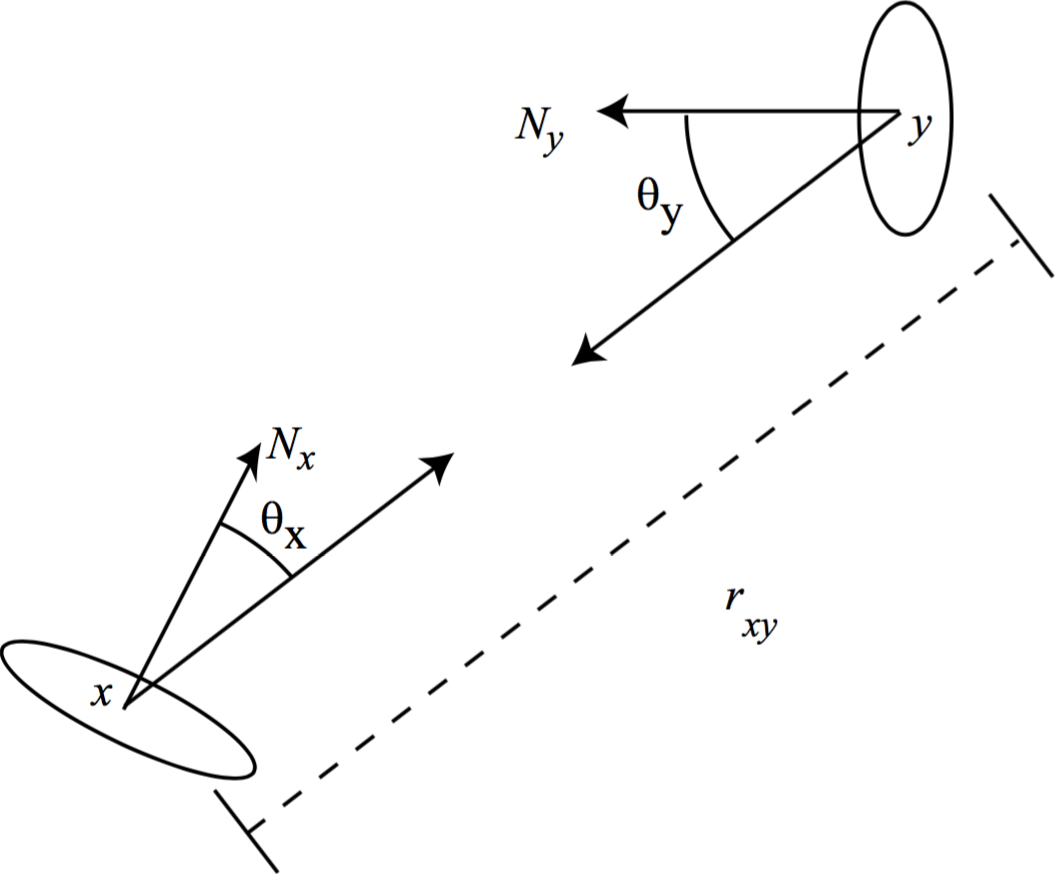
\includegraphics[width=.55\textwidth]{graphics/gi/path-18}
	\caption{辐射亮度由点$y$(实际上是以$y$为中心的单位面积大小的面积)向点$x$传输的几何关系图,辐射亮度实际上是单位面积上的辐射通量,所以辐射亮度的传输必须在垂直于传输方向的面上,这涉及两次面积的投影,以及辐射亮度随着传播距离$r^{2}_{xy}$的增加而衰减,即式\ref{e:r-kernel-k}中的$G(x,y)$项}
	\label{f:r-the-geometry-of-the-surfaces}
\end{figure}

辐射度(radiosity)表示的是光离开一个表面的辐射能量,在一个漫反射环境中,辐射度和出射辐射亮度的关系可以表述为$B(x)=\pi L(x)$和 $B_e(x)=\pi L_e(x)$,对式\ref{e:r-radiosity-temp}两边同时乘以$\pi$就可以得到辐射度积分方程:

\begin{equation}\label{e:radiosity-integral-equatoin}
	B(x)=B_e(x)+\rho(x)\int_S K(x,y)B(y){\rm d}A_y
\end{equation}

\noindent 上式表述的是表面上点$x$处(所在的单位面积)的辐射度,对于任意一个面积$A_i$的曲面片$i$,其所有点发射辐射度的平均值$B_i$可以表述为:

\begin{equation}\label{e:average-radiosity}
	B_i= \cfrac{1}{A_i}\int_{S_i}B(x){\rm d}A_x
\end{equation}

\noindent 即面积$A_i$的曲面上的平均辐射度等于辐射度$B(x)$在该面面积$S_i$上的积分除于该面的面积,如果假设每个曲面$i$上各处的辐射度$B(x)$为常数,即$B(x)=B^{'}_{i},x\in S_i$,则上式可以转化为一个如下的线性方程组:

\begin{equation}\label{e:r-assuming-constant-radiosity}
\begin{aligned}
	B_{i}^{'}=&B_i= \cfrac{1}{A_i}\int_{S_i}B(x){\rm d}A_x\\
			 =& \cfrac{1}{A_i}\int_{S_i}B_e(x){\rm d}A_x+ \cfrac{1}{A_i}\int_{S_i}\int_S \rho (x)K(x,y)B(y){\rm d}A_y{\rm d}A_x\\	
			 =& \cfrac{1}{A_i}\int_{S_i}B_e(x){\rm d}A_x+\sum_j  \cfrac{1}{A_i}\int_{S_i}\int_{S_j} \rho (x)K(x,y)B(y){\rm d}A_y{\rm d}A_x\\
			 =&B_{ei}+\sum_j B_{j}^{'} \cfrac{1}{A_i}\int_{S_i}\int_{S_j} \rho (x)K(x,y){\rm d}A_y{\rm d}A_x
\end{aligned}
\end{equation}

\noindent 对于上式,我们进一步假设每个曲面$i$内各处的反射系数为一个常数,即$\rho(x)=\rho_i,x\in S_i$,则我们可以得到下述的经典辐射度线性方程:

\begin{equation}\label{e:r-radiosity-system-of-equations}
	B_{i}^{'}=B_{ei}+\rho_i\sum_j F_{ij}B^{'}_{j}
\end{equation}

\noindent 其中:

\begin{equation}\label{e:r-form-factor}
	F_{ij}= \cfrac{1}{A_i}\int_{S_i}\int_{S_j}K(x,y){\rm d}A_y{\rm d}A_x
\end{equation}

\noindent 系数$F_{ij}$称为形状系数(form factor)\myindex{形状系数}{form factor},它表示曲面$j$向整个空间发射的辐射能量中落于曲面$i$上的分数部分,我们将在下一节讨论它的一些特性以及计算方法。

以上,我们将漫反射光照的传输转换为了一个基于细分曲面片的线性方程组,由后面的内容可知这个线性方程组可以被高效地求解,从而对于任意给定光照配置(包括自发光物体和光源),我们可以快速计算出场景中每个顶点处的漫反射辐射亮度。

\begin{figure}
	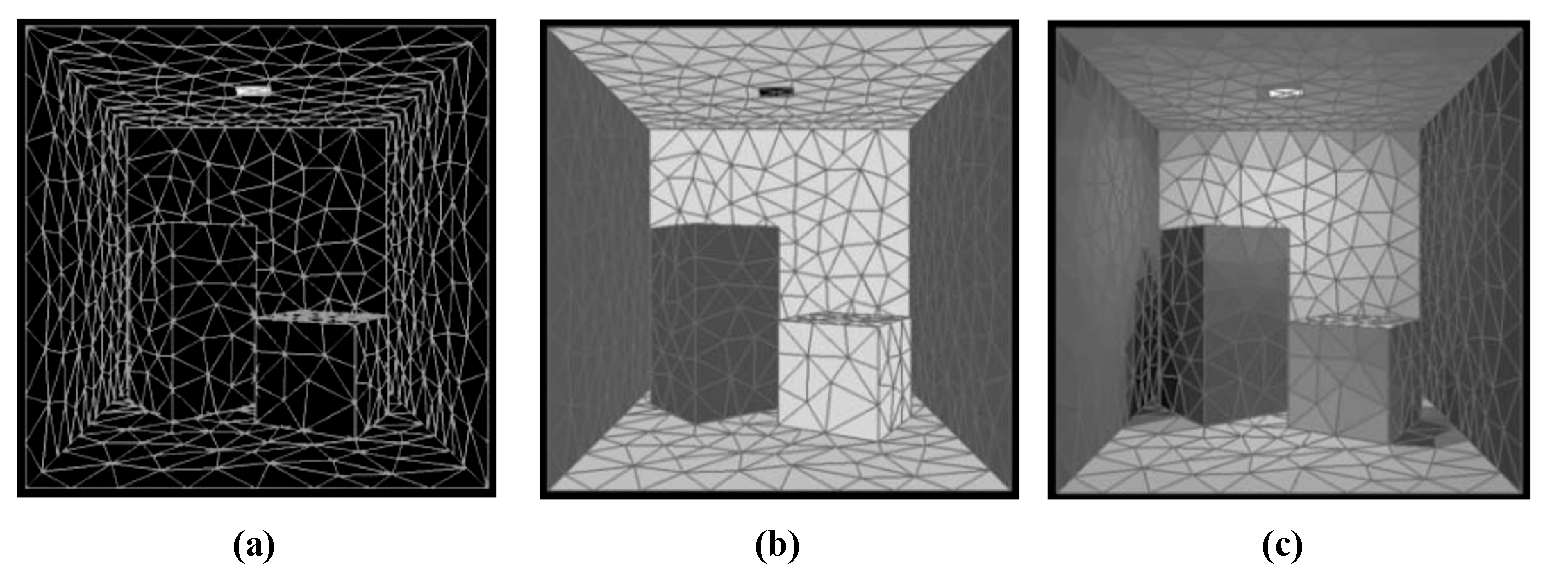
\includegraphics[width=1.\textwidth]{graphics/gi/path-19}
	\caption{经典的辐射度方法的输入数据是一个曲面(例如这里的三角形)列表,以及每个曲面$i$的平均自发光辐射度$B_{i}^{e}$(左),以及每个曲面的漫反射系数$\rho_i$(中),这些信息便被用于计算每个曲面的平均辐射度$B_i$(右)}
	\label{f:r-radiosity-system-of-equations}
\end{figure}

由此,我们可以总结出辐射度方法的一般思路。经典的辐射度方法是一种称为有限元方法(finite element methods,EFM)\mathindex{有限元方法}{finite element methods}的一个应用,如图\ref{f:r-radiosity-system-of-equations}所示,它首先将整个场景细分为一个曲面列表,根据表面漫反射光照的分布情况,这些曲面可以是原始的物体输入数据(例如三角形网格),也可能原始的输入曲面被细分或者合并为其他的曲面片;然后它计算每对曲面片之间的形状系数$F_{ij}$;最后计算整个辐射度线性方程组并提取和使用每个曲面片的辐射度$B_i$;由于原始表面是具有更高分辨率的结构,因此需要使用双线性插值计算每个表面点处的辐射度值。

辐射度方法通常有两种不同的使用方法,首先第一种是传统的用于提升间接漫反射光照的计算效率,此时形状系数在每一帧都被重新计算,以适应场景中物体的动态调整,由于形状系数的计算成本非常高,在第\ref{sec:r-mc-radiosity}节将看到我们甚至可以不用直接计算形状系数就可以使用辐射度方法计算表面的间接漫反射光照。

辐射度方法的第二种运用是用于计算实时渲染场景中的间接漫反射光照传输。首先场景对应的形状系数矩阵被提前预计算并缓存起来,然后在运行时通过求解辐射度线性方程组实时地计算间接漫反射光照传输,这种情况下光源(例如修改光源光照的密度,以及开关各个自发光物体的光照等)和材质属性(例如修改材质的漫反射系数$\rho$)都可以在运行时被动态改变。但是正是由于形状系数的缓存,它只能处理静态场景,但是我们(在第\ref{sec:r-enlighten}节)将介绍一些方法使辐射度方法可以结合其他一些方法来处理动态物体的间接漫反射光照,同时我们也会(在第\ref{sec:r-dynamic-radiosity}节)直接扩展辐射度方法用以处理实时渲染中的动态场景。

上述的过程虽然看起来很简单,但是仍然涉及很多比较棘手的问题,首先是关于形状系数的计算,如式\ref{e:r-form-factor},它包含对两个曲面片上面积的积分,我们将在下一节讨论各种计算形状系数的方法;其次,对于式\ref{e:r-radiosity-system-of-equations}的辐射度线性方程组,其可能包含数量非常巨大的曲面片数量,我们需要高效的求解方法以满足实时渲染的需求,第\ref{sec:r-solving-linear-equations}将会讨论这些方法;最后,通过解决式\ref{e:r-radiosity-system-of-equations}的线性方程组后得到的辐射度$B^{'}_{i}$只是对整个曲面片$i$的平均辐射度(式\ref{e:average-radiosity})的一个近似值, 它的精度取决于细分曲面内漫反射光照的频率变化,例如对于阴影的边缘,即使物体表面的漫反射系数为常数,但是其辐射度的值在该曲面片内变化加大,此时最好的方法是根据阴影的边界对曲面进行划分,然而这需要事先知道光照的分布,而这正是我们要求解的结果,第\ref{sec:r-meshing}节会讨论各种曲面细分方法。





\section{形状系数}\label{sec:r-form-factors}
辐射度方法来源于热能传输(heat transfer)\myindex{热能传输}{heat transfer}的运用中,在热能传输中形状系数$F_{ij}$又称为几何视角系数(geometrical view factor)\myindex{几何视角系数}{geometrical view factor},它指示曲面片$i$中的入射辐射照度有多少部分来自于曲面片$j$。由于漫反射光照是均匀地分布于空间各个方向,因此曲面$j$向曲面$i$发射的能量分量取决于从曲面$j$观察到曲面$i$所占空间的比例,这也是它被称为几何视角系数的原因,它的值取决于曲面之间的空间几何关系。

形状系数具有以下性质:

\begin{itemize}
	\item 在一个闭合的场景中,形状系数的值都是非负的,这是因为式\ref{e:r-form-factor}中的积分值是非负的。当曲面片$i$和曲面片$j$之间不可见时,$F_{ij}=F_{ji}=0$。
	\item 其他任意曲面片$j$到曲面片$i$的所有形状系数$F_{ij}$和的最大值为1:
		\begin{equation}
			\sum_j F_{ij}\begin{cases}
				  =1  & \text{闭合场景}\\
			      <1  & \text{其他}  
				\end{cases}
		\end{equation}
	\item 相关形状系数之间满足互反关系(reciprocity relation)\myindex{互反关系}{reciprocity relation},即:$A_iF_{ij}=A_jF_{ji}$。
\end{itemize}

由于式\ref{e:r-form-factor}表述的形状系数具有两个重叠的面积积分,因此实践中很难通过解析的方法求解,以下我们将介绍两种数值求解方法,第一种称为半立方体方法,第二种则是基于蒙特卡洛方法的求解方法。




\subsection{半立方体方法}\label{sec:the-hemi-cube}
如果两个曲面片$i$和$j$之间的距离相对于它们的尺寸足够大,并且它们之间不存在任何部分被其他物体遮挡,则式\ref{e:r-form-factor}中的内部积分值(即曲面片$j$传输$i$上每个单位面积的分量)几乎保持为常数,因此式\ref{e:r-form-factor}中外部积分表示的平均项可以被去掉,因而得到近似的形状系数为:

\begin{equation}\label{e:r-single-integral}
	F_{ij}\approx F_{\delta ij}=\int_{S_j} \cfrac{cos\Theta_x cos\Theta_y}{\pi r^{2}_{xy}} HID {\rm d}A_j
\end{equation}

\noindent 这里HID函数表面曲面片$i$与$j$之间的可见性,其值为1或0(如果曲面片$i$和$j$不可见),如果两个曲面片足够近或者存在部分遮挡,我们可以将其进行进一步细分成更小的曲面片,以满足上述的条件,第\ref{sec:r-meshing}节将会介绍一些这样的细分方法。

\begin{figure}
\sidecaption
	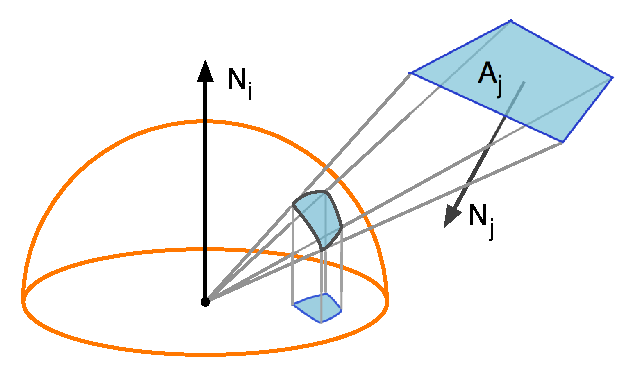
\includegraphics[width=.5\textwidth]{figures/r/nusselt-analog}
	\caption{由于漫反射光照的沿各个方向均匀分布,所以曲面片$j$到曲面片$i$的形状系数$F_{ij}$的值取决于曲面片$i$的面积在曲面片$i$对应单位半球上的投影面积占半球面积的比例,$F_{ij}$的值等于该比例与曲面片$i$的面积$A_i$的乘积}
	\label{f:r-nusselt-analog}
\end{figure}

基于上述的假设,可以使用努赛尔类比(Nusselt analog)\myindex{努赛尔类比}{Nusselt analog}形象地表述出形状系数积分(式\ref{e:r-single-integral})对应的几何关系,如图\ref{f:r-nusselt-analog}所示,首先由于曲面间的距离足够大,因此曲面$j$对曲面$i$上各个点处的光照贡献可以近似为常数,所以这里可以用曲面$i$上单个点的接受光照来表述曲面$j$对其的光照贡献,但也因此其结果还要乘以曲面$i$的面积$A_i$;其次,曲面$j$对于曲面$i$上任意单个点(单位面积)的光照贡献等于其面积$A_j$在该点所在单位半球面上的投影(其值等于固体角),再垂直投影到单位圆上的面积与单位圆面积的比值;当然,如前所述,总的形状系数的值等于该比值与曲面$i$的面积$A_i$的乘积。

从形状系数的定义可知,对于场景中的任意两个曲面$j$和$k$,如果它们投影到曲面$i$所在的半球面上的面积和位置均相等,则它们的形状系数相等,即$F_{ij}=F_{ik}$,如图\ref{f:r-hemicube}(a)所示。

由于到曲面(如图\ref{f:r-nusselt-analog}上的半球面)的投影的计算相当复杂,然而根据上述性质,如果我们能够找到一个投影计算非常简单的“中间曲面”,则我们可以首先将复杂曲面投影到该中间曲面上,然后在将该中间曲面上的投影面积投影到单位圆上。由此\cite{a:Thehemi-cube:aradiositysolutionforcomplexenvironments}提出了半立方体方法,它围绕曲面的中心构造一个假想的半立方体(hemi-cube)\myindex{半立方体}{hemi-cube},如图\ref{f:r-hemicube}(b)所示,该半立方体上的各个面根据一定的分辨率被细分成多个方块像素,例如这个分辨率通常位于$50\times 50$到$100\times 100$之间, 然后曲面被分别投影到半立方体的5个平面上。

\begin{figure}
	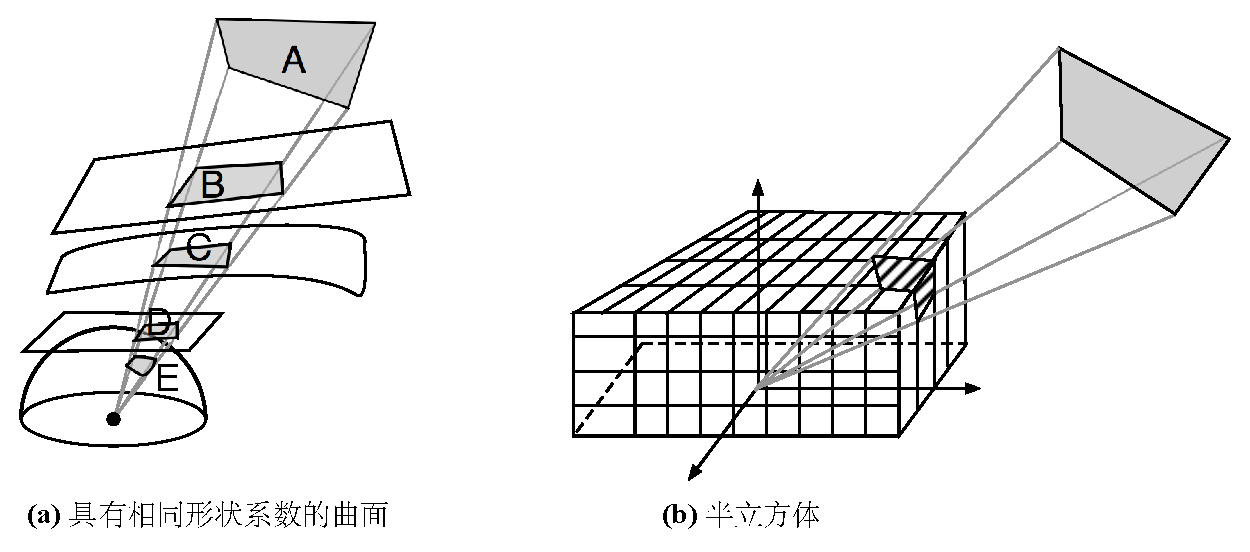
\includegraphics[width=1.\textwidth]{figures/r/hemi-cube}
	\caption{根据形状系数的定义,投影到相同半球面上相同位置相同面积的不同曲面具有形状系数的值是相同的(a),然而投影到曲面上的计算是非常复杂的,所以我们可以使用一个简单的立方体,首先将曲面投影到立方体上,然后再将立方体上的投影面积投影到单位圆上(b)}
	\label{f:r-hemicube}
\end{figure}

在半立方体方法中,曲面到半立方体的投影是通过光栅化的方法计算的,它对半立方体的每个平面执行一次光栅化渲染,摄像机被放置在曲面$i$上的中心位置,如图\ref{f:r-hemicube}(b)所示,一个深度缓存用于记录那些里源曲面更近的可见曲面,某个曲面$j$到曲面$i$的投影面积等于该深度缓存上所有曲面$j$所对应像素的面积之和,如图\ref{f:r-hemicube}(b)中半立方体上的阴影面积。

为了计算半立方体上的投影面积到半球面上的投影面积,半立方体上每个方块像素到半球面的投影映射都被预计算到一个表中,因此通过查询表就可以计算出曲面$j$在曲面$i$所在半球面上的投影面积,进而可以计算出其正投影到单位圆上的投影面积,最终计算出每对曲面之间的形状系数$F_{ij}$。




\subsection{蒙特卡洛方法}\label{sec:r-mc-radiosity}
上述的基于半立方体的方法虽然能够高效地计算形状系数,这得益于它能够使用光栅化的方法寻找每个方向上相交的曲面,然而这种算法却存在比较大的误差,首先它以一个像素块大小的尺寸来近似某个方向的曲面在半立方体上的投影,其次它对半立方体上的所有像素对应的方向进行采样,这可能并不符合形状系数的实际分布。

为了更精确地计算形状系数,一些基于蒙特卡洛方法的形状系数计算方法被提出,这些方法通过对某个分布函数进行采样,然后代入形状系数对应的被积函数用于计算每个样本的贡献值,通过这样我们可以使用重要性采样来减少对形状系数估计的方差。这些基于蒙特卡洛方法的算法主要分为两大类:即局部采样方法和全局采样方法,它们分别使用不同的概率密度函数以及不同的估计形式,以下我们分别介绍。





\subsubsection{局部线段}
局部线段(local line)方法\cite{a:AGeneralTwoPassMethodIntegratingSpecularandDiffuseReflection,a:ARayTracingMethodforIlluminationCalculationinDiffuse-SpecularScenes}以单个曲面$i$为中心,然后对某个概率密度函数采样以对形状系数进行估计,其采样的方法是从曲面$i$向某个方向发射光线以寻找该方向上最近的曲面片,所以这种光线又称为局部线段,它是相对于后面介绍的全局线段而言的,如图\ref{f:r-global-vs-local}(b)所示,我们的主要工作是寻找合适的概率密度函数。

原始的形状系数(式\ref{e:r-form-factor})是关于两个曲面片上面积的积分,因此最直观的想法是对两个曲面上的位置均匀采样,这得到一个均匀概率密度函数$p(x,x^{'})= \cfrac{1}{A_iA_j}$,即每次对$A_i$和$A_j$两个面积上的位置进行均匀采样得到一对位置样本$(x,x^{'})$,对于$N$个这样的样本,形状系数的估计为:

\begin{equation}
	F_{ij}\approx \cfrac{1}{N}\sum^{N}_{k=1} \cfrac{1}{A_i} \cfrac{K(x,y)}{ \cfrac{1}{A_iA_j}}= \cfrac{A_j}{N}\sum^{N}_{k=1}K(x,y)
\end{equation}

\noindent 上述的方法显然没有使用任何重要性采样。实际上虽然形状系数$F_{ij}$仅表述的是两个特定曲面$i$和$j$之间的光照传输关系,但是我们的目标实际上是要计算表面上来自于整个半空间的辐射照度,将目光局限于单独两个特定的曲面并无法探索表面漫反射传输的这种全局特性,例如来自于靠近法线方向的曲面的光照贡献显然要大于来自于靠近表面正切面方向的曲面,但是如果使用上述的概率密度则无法为更重要的曲面分配更多的样本以减少估计的方差。为此我们需要对形状系数使用另外一种表述。

对于形状系数$F_{ij}$,曲面$j$对于曲面$i$所提供的信息仅仅是一个在半球面上的投影面积,该面积表示一定大小的固体角,对于给定位置和大小的固体角,曲面$j$可以是任意曲面,如\ref{f:r-hemicube}(a)所示,我们真正所关心的并不是这个固体角来源于哪个曲面的投影,而仅仅是这些方向上是否具有可见的曲面$j$。

由此我们可以将形状系数表示为一个针对半球面(而不是一个特定曲面$j$)的积分,由于曲面面积$A_j$与固体角之间的关系可以表述为${\rm d}\omega= \cfrac{\cos\theta_j}{|x_i-x_j|^{2}}{\rm d}A_j$,所以式\ref{e:r-form-factor}表述的针对曲面积分形式的形状系数可以转化为如下针对半球面的积分形式:

\begin{equation}
	F_{ij}= \cfrac{1}{A_i}\int_{A_i}\int_{\Omega} \cfrac{\cos\theta_i}{\pi}V_j(x_i,\omega){\rm d}\omega {\rm d}A_i
\end{equation}

\noindent 其中,$V_j(x_i,\omega)$表示从$x_i$开始沿$\omega$方向上是否存在一个可见的曲面$j$。有了上述的表述,我们不仅能对半球面方向进行重要性采样,还能通过一个采样过程同时计算所有传输光照至曲面$i$的形状系数$F_{ij}$。

由于固体角${\rm d}\omega$可以使用极坐标表述为$\sin\theta d\theta d\psi$,所以上式也可以表述为:

\begin{equation}\label{e:r-form-factor-over-hemisphere}
	F_{ij}= \cfrac{1}{\pi A_i}\int_{A_i}\int_{\theta}\int_{\psi}V_j(x_i,\theta,\psi)\cos\theta\sin\theta {\rm d}\theta {\rm d}\psi {\rm d}A_i
\end{equation}

\noindent 如果曲面$j$在${\rm d}A_i$沿$(\theta,\psi)$方向上可见,则$V_j(x_i,\theta,\psi)$的值为1,否则为0。

针对上述的形状系数表述形式,重要采样建议的概率密度函数为$p(x,\theta,\psi)= \cfrac{\cos\theta\sin\theta}{\pi A_i}$,其$N$个随机数对应的估计为:

\begin{equation}
	F_{ij}\approx \cfrac{1}{N}\sum^{N}_{k=1} \cfrac{1}{\pi A_i} \cfrac{V_j(x_k,\theta_k,\psi_k)\cos\theta_k\sin\theta_k}{ \cfrac{\cos\theta_k\sin\theta_k}{\pi A_i}}= \cfrac{1}{N}\sum^{N}_{k=1}V_j(x_k,\theta_k,\psi_k)
\end{equation}

这是一个非常简洁的估计,我们甚至不需要计算每个曲面对之间点到点的贡献函数$K(x,y)$中的$G(x,y)$项,它仅剩下一个可见性判断。即我们只需要通过从$i$向整个半球面均匀发射线段,然后统计一下有多少线段落于曲面$j$上,这些落于曲面$j$上线段占据总的线段数量$N$的比例即是对形状系数$F_{ij}$的估计,如图\ref{f:r-global-vs-local}(b)所示。

\begin{figure}
\sidecaption
	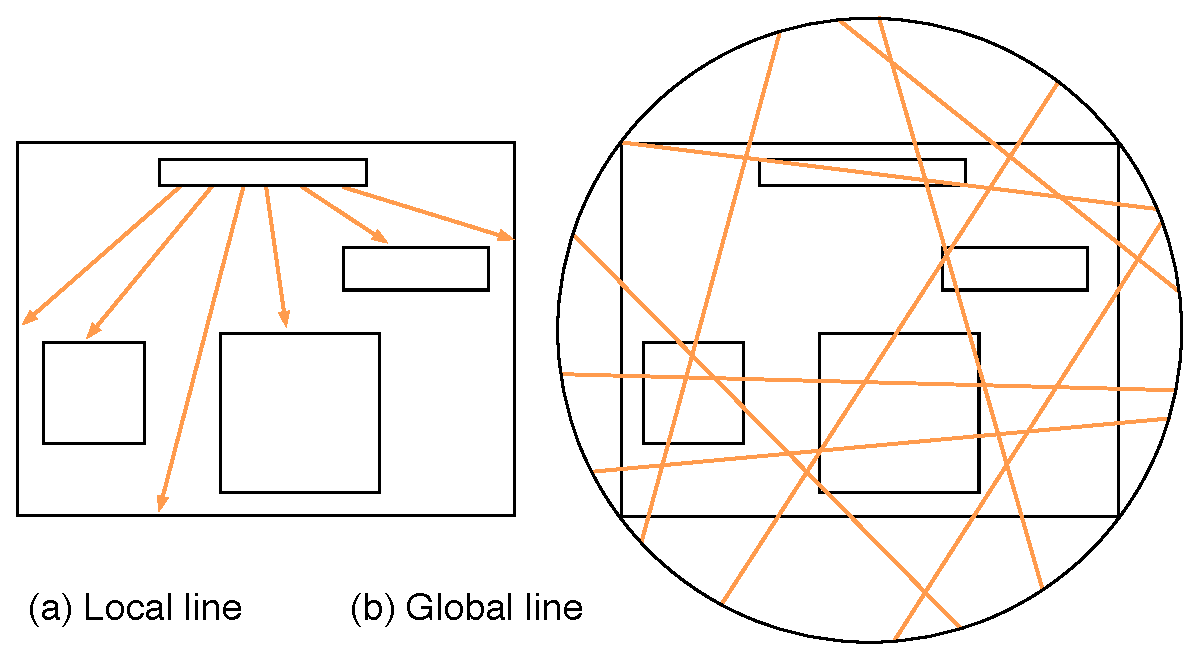
\includegraphics[width=.65\textwidth]{figures/r/global-vs-local}
	\caption{使用蒙特卡洛方法对形状系数进行估计:(a)通过发射局部线段进行估计,形状系数$F_{ij}$的值等于从曲面$i$出发落于曲面$j$上的线段数量占全部线段数量的比例;(b)通过发射全局线段进行估计,可以通过类似的方法统计落于相关曲面对上的线段比例来对形状系数进行估计}
	\label{f:r-global-vs-local}
\end{figure}

上述局部线段蒙特卡洛方法的另一个特性是它能够同时对曲面$i$的所有形状系数$F_{ij}$进行估计,而不是分别对单个形状系数进行估计。

上述的概率密度函数由三部分的乘积组成:

\begin{equation}
	p(x,\theta,\psi)= \cfrac{\cos\theta\sin\theta}{\pi A_i}=p^{1}(x)p^{2}(\psi)p^{3}(\theta)= \cfrac{1}{A_i}\times \cfrac{1}{2\pi}\times 2\cos\theta\sin\theta
\end{equation}

\noindent 其中,$ \cfrac{1}{A_i}$表示对曲面$i$的面积$A_i$上位置的均匀采样,$ \cfrac{1}{\pi}$表示对位置$x$在$(0,2\pi)$上均匀采样获得有一个半空间上的方向$\psi$,对于最后一项,我们可以通过逆向变换法求其样本值,对$2\cos\theta\sin\theta$积分可以得到累积概率密度函数$F(\theta)=\sin^{2}\theta=1-\cos^{2}\theta$,所以通过获得一个[0,1)上均匀分布的随机数$\xi$,其$p^{3}$对应的随机数为$\arcsin(\sqrt{\xi})$。




\subsubsection{全局线段}
根据上述用概率描述形状系数的思路,我们还可以使用全局线段来估计形状系数,如图\ref{f:r-global-vs-local}(b)所示,通过在场景中均匀地发射全局光线,每个光线同时穿越所有该方向上的物体,通过记录哪些互相可见的曲面对对应的全局线段数量,我们可以使用上节类似的线段数量比例的思路对形状系数进行估计。

不过实际上全局线段方法并不单纯是从上述的概念延伸出来的,而是来源于积分几何中相关的知识。积分集合(integral geometry)\mathindex{积分集合}{integral geometry}\cite{b:Integralgeometryandgeometricprobability}通过概率的方式使用一些全局的线段来描述物体的一些积分性质,通过对一个能够包围所有几何体的空间随机均匀地发射一些光线,这些光线均匀地分布于空间中的各个位置,因此这些物体相交光线的数量正比于该物体的表面积,因此所有对于表面积进行积分的问题均可以通过分析这些光线的数量(即概率)来进行估计,例如一个凸面多边形与多少光线相交,有多少条光线与一个表面相交,同时与两个表面相交的光线数量是多少,通过这些光线密度数据,我们就能计算和面积相关的一些积分。

由此,\cite{a:AnIntegralGeometryBasedMethodforFastForm-FactorComputation}提出了基于全局线段的方法,如图\ref{f:r-global-vs-local}(b)所示,它首先对全部场景中的物体使用一个球包围起来,然后每次随机均匀地选取球面上的两个位置并连接形成线段,这些这些全局线段就能均匀分布于整个空间,每个线段与物体表面的相交信息以及每个局部相互可见的曲面对都被记录起来,这样既能使用前面局部线段类似的方法估计形状系数,也能使用积分集合中特定的一些与面积相关的公式来估计形状系数,这里不再进行详细讨论,感兴趣的读者可以进一步阅读\cite{a:TheUseofGlobalRandomDirectionstoComputeRadiosityGlobalMonteCarloTechniques}了解更多信息。

相对于局部线段方法,全局线段方法更容易通过利用线段之间内存的连贯性来提升计算效率,然而其缺点是不能单独提升或降低某个特定曲面的光线密度,在计算形状系数时,其方差大致与其曲面的面积成反比,因此面积较小的曲面其形状系数具有较大的方差,这时局部线段方法可以通过改变特定曲面的线段密度来改善方差分布。





\section{求解线性方程组}\label{sec:r-solving-linear-equations}
形状系数表示的仅仅是光照的传输过程而不是结果,对于曲面对$i$和$j$,$F_{ij}$它表示曲面$i$上的光照能量有多少部分是来自于曲面$j$。由于光照传输是一个递归的过程,因此曲面上的辐射度是一个$n\times n$的线性方程组,如式\ref{e:radiosity-integral-equatoin},其中$n$表示细分曲面的数量,也即是线性方程组中方程的数量以及矢量变量的分量数。

对于包含$n$个未知变量的$n$个线性方程组,数学上常用的求解工具是高斯消元法(Gauss elimination)\mathindex{高斯消元法}{Gauss elimination}或高斯-乔登消元法(Gauss-Jordan elimination)\mathindex{高斯-乔登消元法}{Gauss-Jordan elimination},它们通过对方程组的系数构成的矩阵执行一系列行交换操作将其转换为一个上三角矩阵(upper triangular matrix)\mathindex{上三角矩阵}{upper triangular matrix}进行求解。然而这样精确求解的方法在数字计算机中运用时却会遭遇被称为取整误差带来的问题。

在数字计算中,一个实数被保存为浮点数(floating point)\myindex{浮点数}{floating point}的形式,即$\pm M\times 10^{k}$,这里$k$表示一个整数,$M$表示一个尾数(mantissa)\myindex{尾数}{mantissa},它满足不等式$0.1\leq M<1$,例如以下是一些实数及对应计算机中存储的浮点数:

\begin{equation}
\begin{aligned}
	\text{实数}   &&   \text{浮点数}	\\
	129          &&   0.129\times 10^{3}\\
	-2.13785 	 &&   -0.213785\times 10^{1}\\
	0.00038      &&   0.38\times 10^{-3}
\end{aligned}
\end{equation}

计算机中存储尾数的数字位是有限的,如果有$n$个数字位供存储,那么超出$n$的部分则按四舍五入法进行取整,取整后被存储进计算机的值称为存储值(stored value),例如0.1253被存储为0.13,而0.1247倍存储为0.12,这种由于数字位存储限制导致的误差称为取整误差(rounding error)\myindex{取整误差}{rounding error}。

上述的高斯(-乔登)消元法是由一系列操作组成的,对于每一此操作计算,它都需要将结果写回到内存中供后续的计算使用,每次存储都可能出现这种取整误差,随着整个消元法的进行,这些误差被传播并累计下去,导致最终结果出现比较大的误差,辐射度方法中矩阵的维度更是可能上万,这种误差是不可能忽略的。

高斯消元法计算的是一个直接的结果,它没有提供一种修正的机制,对于这样的误差,我们希望能够有一种修正的机制用于通过一个迭代过程将误差逼近至某个可接受的范围。所以在计算机中,我们通常使用迭代法来求解线性方程组,例如前面介绍的牛顿迭代法,它每次计算的可能不是一个直接准确的结果,但是它提供一种机制使可以逐渐收敛到正确结果,在这个收敛过程中,我们就有机会将最终结果限定在一个可接受的误差范围。

以下将介绍常见的使用迭代法求解线性方程组的方法,在第\ref{sec:r-global-transfer-operator}还会介绍另一种通过直接求解一个全局的传输矩阵的方法来提高辐射度线性方程组计算的效率。




\subsection{迭代法}\label{sec:r-iteration}
最早的迭代算法称为雅可比方法(Jacobi method),对于线性方程组:

\begin{equation}
\begin{aligned}
	a_{11}x_1  &&+&&  a_{12}x_2 && +\cdots + && a_{1n}x_n &&=&& b_1\\
	a_{21}x_1  &&+&&  a_{22}x_2 && +\cdots + && a_{2n}x_n &&=&& b_2\\
	\vdots     && &&  \vdots    &&           && \vdots    && && \vdots\\
	a_{n1}x_1  &&+&&  a_{n2}x_2 && +\cdots + && a_{nn}x_n &&=&& b_n
\end{aligned}
\end{equation}

\noindent 对于上述方程组,雅可比方法的计算基于两个假设:首先上述的线性方程组有唯一解,其次其系数矩阵$A$的对角线均由非零值组成,如果任意一个对角线上的项$a_{11},a_{22},\cdots,a_{nn}$的值为0,则需要执行行或列的交换操作使其对角线上的项不为0。

为了开始执行雅可比方法,首先需要对上述的方程组执行一个操作以提取出每个未知量$x_i$的表达式:

\begin{equation}\label{e:r-jacobi-approximation}
\begin{aligned}
	x_1 && =     &  \cfrac{1}{a_{11}}(b_1-a_{12}x_2-a_{13}x_3-\cdots -a_{1n}x_n)\\
	x_2 && =     &  \cfrac{1}{a_{22}}(b_2-a_{21}x_1-a_{23}x_3-\cdots -a_{2n}x_n)\\
	    &&\vdots &\\
	x_n && =     &  \cfrac{1}{a_{nn}}(b_n-a_{n1}x_1-a_{n2}x_3-\cdots -a_{n,n-1}x_{n-1})\\
\end{aligned}
\end{equation}

\noindent 上式形成了一个原始方程组解的初始近似,例如对于任意一组初始值$(x_1,x_2,x_3,\cdots,x_n)$都可以看做是方程组解的一个近似,这个近似的误差很大,但是我们可以将这样的初始值加入式\ref{e:r-jacobi-approximation}的右边,可以得出一个更好的近似,以这样的方法形成迭代,则方程组的解可以逼近真实解,这就是雅可比方法的思路。

利用上述方法,例如对于一个线性方程组:

\begin{equation}
\begin{aligned}
	5x_1  && - && 2x_2 && + && 3x_3 && = && -1\\
	-3x_1 && + && 9x_2 && + && x_3  && = && 2\\
	2x_1  && - && x_2  && - && 7x_3 && = && 3
\end{aligned}
\end{equation}

可以得到如表\ref{t:r-jacobi-iteration}所示的迭代序列,运用这样的迭代方法,每个迭代都是比上一个迭代更好的近似,所以很快逼近到真实值。

\begin{table}
\caption{一个雅可比迭代序列,给定一个初始近似值$(x_1,x_2,x_3)=(0.000,0.000,0.000)$,运用雅可比迭代法,每次迭代是比前一迭代更好的近似,所以可以很快收敛到正确的值}
\label{t:r-jacobi-iteration}
\begin{tabular}{p{0.1\textwidth}|p{0.1\textwidth}|p{0.1\textwidth}|p{0.1\textwidth}|p{0.1\textwidth}|p{0.1\textwidth}|p{0.1\textwidth}|p{0.1\textwidth}|p{0.1\textwidth}}
\hline 
   n & 0 & 1 & 2 & 3& 4& 5 &6 & 7 \\
    \hline  
  $x_1$ & 0.000 & -0.200 & 0.146  & 0.191  & 0.181  & 0.186  & 0.186  & 0.186\\
  $x_2$ & 0.000 & 0.222  & 0.203  & 0.328  & 0.332  & 0.329  & 0.331  & 0.331\\
  $x_3$ & 0.000 & -0.429 & -0.517 & -0.416 & -0.421 & -0.424 & -0.423 & -0.423\\
 \hline 
\end{tabular}
\end{table}




\subsubsection{高斯-赛德尔方法}\label{sec:r-gauss-seidel-iteration}
实践中常使用雅可比方法的一种变种\cite{a:ModelingtheInteractionofLightBetweenDiffuseSurfaces},称为雅可比-赛德尔方法(Gauss-Seidel method)\mathindex{雅可比-赛德尔方法}{Gauss-Seidel method},对于每次迭代中的$x_i$的值,由于所有索引小于$i$的未知量$x_1,\cdots,x_{i-1}$的值都会被用在下一迭代中方程组的右边,所以雅可比-赛德尔方法就直接将当前迭代中所有计算出的$x_i$的值用在后续的$x_{i+1},\cdots,x_n$的计算中,这样加快了雅可比方法的迭代速度,如表\ref{t:r-jacobi-seidel-iteration}所示。

\begin{table}
\caption{一个雅可-赛德尔比迭代序列,相较于雅可比方法,由于在每次迭代中它将$x_i$的计算结果直接用在后续的未知量的计算中,这相当于提前了某些迭代的计算,因此迭代效率得到提升}
\label{t:r-jacobi-seidel-iteration}
\begin{tabular}{p{0.1\textwidth}|p{0.1\textwidth}|p{0.1\textwidth}|p{0.1\textwidth}|p{0.1\textwidth}|p{0.1\textwidth}|p{0.1\textwidth}|p{0.1\textwidth}|p{0.1\textwidth}}
\hline 
   n & 0 & 1 & 2 & 3& 4& 5 &6 & 7 \\
    \hline  
  $x_1$ & 0.000 & -0.200 & 0.167  & 0.191  & 0.187  & 0.186  & 0.186  & 0.186\\
  $x_2$ & 0.000 & 0.156  & 0.334  & 0.334  & 0.331  & 0.331  & 0.331  & 0.331\\
  $x_3$ & 0.000 & -0.508 & -0.422 & -0.422 & -0.422 & -0.423 & -0.423 & -0.423\\
 \hline 
\end{tabular}
\end{table}



%\subsection{全局传输操作符}\label{sec:r-global-transfer-operator}





\section{曲面细分}\label{sec:r-meshing}
在上面的经典辐射度方法中,我们将整个场景中的几何表面划分成多个曲面,并假设每个曲面内每个点的辐射度近似为一个常数,因此一个曲面向另一个曲面的辐射度可以表示成该曲面内的(常数)辐射度和形状系数的乘积,如式\ref{e:r-assuming-constant-radiosity}所示,进一步假设曲面内的漫反射系数为常数,则整个场景内辐射度的传输可以转换为一个如式\ref{e:r-radiosity-system-of-equations}的线性方程组,所以我们只要通过第\ref{sec:r-form-factors}节介绍的方法求解出式\ref{e:r-radiosity-system-of-equations}中的形状系数$F_{ij}$(如式\ref{e:r-form-factor}),然后可以通过第\ref{sec:r-solving-linear-equations}节介绍的方法求解辐射度线性方程组,从而计算出每个表面的漫反射光照。

然而,由于物体之间(或内部)的遮挡形成阴影等因素,曲面内的辐射度并不总是能够被近似为常数,尽管理论上我们总是可以通过划分更小的曲面来克服这样的问题,但是由于形状系数的存储复杂度为$\mathcal{O}(n^{2})$(其中$n$为曲面的数量),高分辨率的曲面细分会使得整个辐射度计算的性能大大降低。

另一方面,传统按固定尺寸划分曲面的细分方法的精确度有些超出了实际的精度需求,例如由于每个曲面都被细分成相似的面积,因此所有曲面$j$对于曲面$i$的能量贡献与距离的平方成反比,那些较远的曲面的能量贡献远远小于较近物体(甚至可以忽略不计),但是它们却被使用了相同的计算和存储资源。

由于传统辐射度方法存在上述低效的部分,所以本节从形状系数的分布特征着手,寻找在使用最小的计算和存储资源的条件下,实现同等质量辐射度计算的方法。

这些方法涉及非均匀的曲面细分(例如它们根据形状系数的分布对每个曲面$i$相对于不同距离的曲面$j$使用不同的曲面尺寸),这可以分为两大类方法:第一类称为后验方法(a posteriori),这类方法首先建立一个粗粒度的网格划分,然后根据相关信息对曲面进行进一步划分,比较典型的如阶层式辐射度方法(第\ref{sec:r-hierarchical-radiosity}节);另一类称为先验方法(a priori)它首先主要是根据辐射度分布的不连续性,例如阴影边缘等,产生一些边沿点,然后细分过程根据这些点进行细分,例如非连续网格化(第\ref{sec:r-discontinuity-meshing}节)。最后,我们会介绍这两类不同思路方法的组合方法。

特别地,我们还会从数学的角度给予上述这些细分方法一个更合理的解释,它们其实是来源于数字信号处理里面的一些思路,这有助于我们更深刻地理解这些曲面细分方法。




\subsection{阶层式辐射度方法}\label{sec:r-hierarchical-radiosity}
本节我们首先介绍最基本的阶层式辐射度方法的基本原理和思路,然后在第\ref{sec:r-wavelet-based}节说明这种基本的阶层式辐射度方法其实是一种基于小波分析的数字信号处理方法的一种特殊情况,基于小波分析的辐射度方法给出了阶层式辐射度方法更一般的数学解释。




\subsubsection{基本算法}
基本的阶层式辐射度方法来源于物理学中的N-体问题(N-body problem)\myindex{N-体问题}{N-body problem}\cite{a:AnEfficientProgramforManyBodySimulation},它用于预测星体(如太阳,月亮,地球及其他可见行星)在相互引力作用下的运动。在N-体问题中(N为总的待预测行星数量),每个行星都对其他N-1个行星施予引力作用,这产生N(N-1)/2中相互交互,这和曲面之间通过形状系数相互作用相似,N-体问题通过利用以下思路使得总的计算时间小于平方时间($\mathcal{O}(n^{2})$):

\begin{enumerate}
	\item 数值计算方法总是包含一定的误差,所以每个星体的引力计算只要被限制在一定的精度即可。
	\item 对于较远距离的一个行星簇(包含多个相邻行星),它们的引力效果可以被近似为一个单一的项(例如看成一个更大体积的“星体”),这也是因为引力和距离的平方成反比,这大大减少了需要计算的总的交互的数量。
\end{enumerate}

这两点思路同样可以被用于辐射度方法,\cite{a:ARapidHierarchicalRadiosityAlgorithm}基于此提出了阶层式辐射度方法(hierarchical radiosity)\myindex{阶层式辐射度方法}{hierarchical radiosity},与经典辐射度方法将整个场景细分成固定面积尺寸大小的曲面片不同,阶层式辐射度方法是一个迭代细化的过程,它将每个多边形几何表面分解为由曲面和元素组成的一个阶层结构,相当于每个曲面被按多个不同的分辨率进行细化,整个阶层结构使用一个四叉树保存,四叉树的每个层级对应一个分辨率,这里将所有非叶节点称为曲面,而将叶节点称为元素(element),这有点类似于几何体表面的多级纹理,每一级纹理使用不同的分辨率表述同一个表面。

阶层式辐射度方法中对曲面的迭代细分如算法\ref{a:r-hierarchical-radiosity}所示。

\begin{algorithm}
\begin{lstlisting}[language=C++, mathescape]
void Refine(Patch *p, Patch *q, float $F_{eps}$, float $A_{eps}$) {
	float $F_{pq},F_{qp}$;
	
	$F_{pq}$ = FormFactorEstimate(p, q);
	$F_{qp}$ = FormFactorEstimate(q, p);
	
	if($F_{pq}<F_{eps}$ && $F_{qp}<F_{eps}$) 
		Link(p,q);
	else {
		if($F_{pq}>F_{qp}$){
			if(Subdiv(q, $A_{eps}$)){
				Refine(p,q->ne, $F_{eps}$, $A_{eps}$);
				Refine(p,q->nw, $F_{eps}$, $A_{eps}$);
				Refine(p,q->se, $F_{eps}$, $A_{eps}$);
				Refine(p,q->sw, $F_{eps}$, $A_{eps}$);
			}
			else 
				Link(p, q);
		}
		else {
			if(Subdiv(p, $A_{eps}$)){
				Refine(q,p->ne, $F_{eps}$, $A_{eps}$);
				Refine(q,p->nw, $F_{eps}$, $A_{eps}$);
				Refine(q,p->se, $F_{eps}$, $A_{eps}$);
				Refine(q,p->sw, $F_{eps}$, $A_{eps}$);
			}
			else 
				Link(p, q);
		}
	}
}
\end{lstlisting}
\caption{阶层式辐射度方法将每个曲面划分成多个分辨率的细分结构,这形成一个类似多级纹理的阶层结构,整个结构用一颗四叉树表述,四叉树内的所有节点(包括不同层级的节点)之间都可以形成形状系数,所有形状系数仅被限定在一定的误差范围(即$F_{eps}$),所有超出这个精细度的形状系数则被忽略,这大大减少了实际需要计算的形状系数的数量,并且能够保证估计的精度需求}
\label{a:r-hierarchical-radiosity}
\end{algorithm}

阶层式辐射度方法的主要思路是在保证一定精度(如这里的$F_{eps}$)的情况下,将那些高于这个精度的形状系数忽略掉来近似整个形状系数函数的分布,这能够实现的原因是因为形状系数与曲面之间的距离的平方成反比,所以那些较远距离的精细曲面(即元素)形成的形状系数值非常小以至于可以被忽略,取而代之的是可以使用一个更低分辨率的曲面来代替,这样就减少了需要保存的形状系数矩阵元素的数量。

为此,算法\ref{a:r-hierarchical-radiosity}首先比较两个曲面$p$和$q$之间的真实形状系数$F_{pq}$和$F_{qp}$(这可以通过第\ref{sec:r-form-factors}节介绍的方法计算而出)是否小于指定的误差范围$F_{eps}$,如果两者都小于该范围,则记录这两个形状系数到形状系数矩阵用于后面的线性方程组的求解计算;否则,对形成形状系数较大的曲面进行进一步细分,首先将该较大的曲面均分成4个子曲面,这通过调用Subdiv()方法实现,每个子曲面这里存储为四叉树中的四个子节点指针$x\to ne,x\to nw,x\to se,x\to sw$(这里$x$表示父节点),然后计算每个小曲面与另一个较小曲面之间的形状系数;上述的过程迭代进行,直到满足终止条件。

除了$F_{eps}$的终止条件,算法\ref{a:r-hierarchical-radiosity}也限制每个叶节点元素的面积下限,当待细分的曲面面积小于$A_{eps}$时,则迭代终止,对应的形状系数被强制记录,这可以防止如边角处的曲面的迭代无限进行下去。

图\ref{f:r-hierarchical-interactions}显示了阶层式辐射度方法中曲面细分的一个例子,这里为了方便解释,仅使用了两个相互垂直的曲面,每个曲面被按照不同的分辨率划分成成多个曲面细分结构,所有细分结构被使用一个四叉树组合起来,从这里可以看到,仅有那些比较靠近的曲面之间的形状系数的计算才会使用高分辨率的细分曲面,对于较远距离的曲面,它们之间的形状系数的计算会使用更低分辨率的曲面,而数量众多的高分辨率的曲面则被忽略,这大大降低了最终被用于线性方程组计算的形状系数矩阵的元素的数量,在一些情况下这甚至可以达到$\mathcal{O}(n)$的存储复杂度。

\begin{figure}
\begin{fullwidth}
	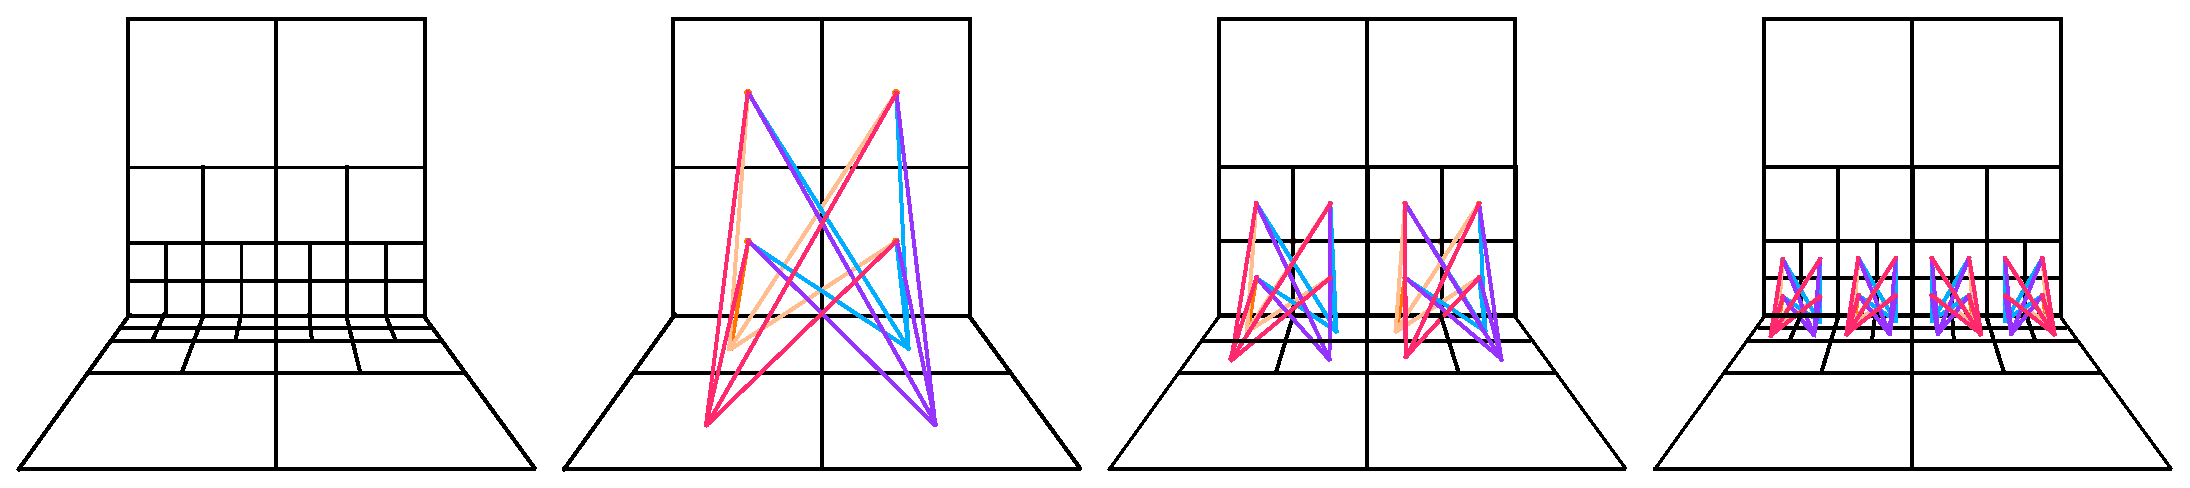
\includegraphics[width=1.0\thewidth]{figures/r/hierarchical-interactions}
	\caption{两个相互垂直平面曲面的阶层式细分,每个曲面被按照多个分辨率细分成不同的结构,较远的曲面之间的形状系数的计算只使用较低分辨率的结构中,这能够在忽略贡献值较小的曲面之间的形状系数的同时,保证形状系数估计的精确度}
	\label{f:r-hierarchical-interactions}
\end{fullwidth}
\end{figure}

对于上述形状系数矩阵的计算,有一个概念是容易产生混淆的,即对于曲面$i$和$j$之间的形状系数$F_{ij}$的计算,假设$i$和$j$之间的距离非常远,我们可能会认为仅有$j$曲面是一个更低分辨率“组合”曲面,而$i$仍维持为一个精细曲面,即四叉树的叶节点,如果是这样的话则发生交互的曲面对数量仍然为$n$,和经典辐射度方法一样,这里的$n$表示所有精细曲面的数量,也即四叉树中叶节点的数量,所以并不能节省曲面对的数量。

实际上注意在算法\ref{a:r-hierarchical-radiosity}中,每个曲面对从最低分辨率的原始曲面开始迭代细分,如果将这个过程看做是一个四叉树的遍历的话,和传统的遍历算法不一样的是,这里的遍历并不一定会到达叶节点,其遍历的终止条件是任何时刻相互的形状系数$F_{pq}$和$F_{qp}$同时小于$F_{eps}$。这样的结果是曲面之间的交互通常发生于四叉树的同一层级内,例如在图\ref{f:r-hierarchical-interactions}中,由于两个曲面的面积相同,因此每个分辨率下的每个曲面节点的面积也相同,这样同层级之间相互的形状系数的值通常相近,因此它们容易在同一层级满足终止条件,这使得发生交互的曲面对通常仅发生在同一层级内,这阻止了跨层级之间的曲面交互,这样才能够降低曲面之间交互的数量。

由于最终的形状系数矩阵中的元素包含了所有层级中的曲面,因此表面上每个点不再唯一对应一个曲面,而是对应不同分辨率下的多个曲面,因此表面上每个点最终的辐射度值应该是所有覆盖该点的曲面的辐射度值的和,对于每一个曲面,它遍历该曲面所有的父节点直至根节点以计算所有分辨率下曲面的辐射度值。

上述的方法仍然忽略了可见性的计算,即假设所有(不同分辨率)曲面之间都是全部可见的,我们将在第\ref{sec:r-discontinuity-meshing}节讨论可见性带来的影响及其处理方法。





\subsection{基于小波的辐射度方法}\label{sec:r-wavelet-based}
上一节我们从几何直觉的角度介绍了阶层式辐射度方法,它将物体表面分解为多个不同分辨率的细分曲面阶层结构,然后对于较远距离之间的曲面,它通过使用更低分辨率的曲面来代替那些固体角非常小以至于可以忽略的精细曲面,从而大大降低了曲面之间交互的数量,提高了辐射度线性方程组求解的效率。

本节我们将说明,实际上这样的思路正是信号处理中小波分析的核心机制,通过对小波辐射度方法的学习,我们将会看到阶层式辐射度方法正是小波辐射度方法中一种特殊的情况--即使用哈尔函数作为基函数对函数进行处理,有了小波分析的理论,我们还可以演变出非常多不同的处理方法,例如使用不同的基函数,以及对于每个基函数使用不同的阶,这些不同的选择都对小波辐射度方法的计算效率有着不同的影响。

为了更好地理解小波辐射度方法(第\ref{sec:r-wavelet-radiosity}节)的思路,我们需要首先简要介绍一些小波分析(第\ref{sec:r-wavelets}节)的内容,而为了理解小波分析的机制,我们需要首先简要复习一下内积和正交投影的概念。




\subsubsection{内积和正交投影}\label{sec:r-inner-product-and-projections}
普通的内积是一个矢量空间(包括实矢量和复矢量空间)中定义的一种操作,就像实数空间的加减乘除操作一样,对于任意一个$n$维的向量空间$V$上的两个矢量$\mathbf{x}=(x_1,x_2,\cdots,x_n)$和$\mathbf{y}=(y_1,y_2,\cdots,y_n)$,其内积(inner product)\mathindex{内积}{inner product}定义为:

\begin{equation}\label{e:r-inner-product}
	\langle \mathbf{x},\mathbf{y}\rangle =\sum^{n}_{j=1}x_jy_j
\end{equation}

\noindent 上式的结果是一个标量,即矢量空间$V$上的内积是一个映射函数$\langle\cdot,\cdot\rangle:V\times V\to F$。对于所有矢量$\mathbf{u},\mathbf{v},\mathbf{w}\in V$以及标量$a\in F$,内积具有以下性质:

\begin{enumerate}
	\item 正性:$\langle \mathbf{v},\mathbf{v}\rangle\geq 0$,且当且仅当$\mathbf{v}=\mathbf{0}$时,$\langle \mathbf{v},\mathbf{v}\rangle= 0$。
	\item 共轭对称性:$\overline{\langle \mathbf{v},\mathbf{w}\rangle}=\langle \mathbf{w},\mathbf{v}\rangle$。
	\item 均匀性:$\langle c\mathbf{v},\mathbf{w}\rangle=c\langle \mathbf{v},\mathbf{w}\rangle$。
	\item 线性:$\langle \mathbf{u}+\mathbf{v},\mathbf{w}\rangle=\langle \mathbf{u},\mathbf{w}\rangle+\langle \mathbf{v},\mathbf{w}\rangle$
\end{enumerate}

定义了内积的矢量空间称为内积空间(inner product space)\mathindex{内积空间}{inner product space}。注意,这里内积的正性意味着可以使用一个矢量同自己的内积来定义矢量的长度,即$||\mathbf{v}||=\sqrt{\langle \mathbf{v},\mathbf{v}\rangle}$,矢量的长度又称为范数(norm)\mathindex{范数}{norm};而长度的定义意味着两个矢量之间的距离可以定义为$||\mathbf{v}-\mathbf{w}||$,因此内积的正性还意味着当$||\mathbf{v}-\mathbf{w}||=0$时,只有$\mathbf{v}=\mathbf{w}$,这在后面理解正交投影时非常有用(即到某个基正交投影后的矢量距离原矢量的距离最短,因此是在该基上对原矢量最好的近似)。

对于$\mathcal{R}^{3}$中的内积,根据余弦定理$|\langle\mathbf{x},\mathbf{y}\rangle |=||\mathbf{x}|||\mathbf{y}|||\cos(\theta)|$,其中$\theta$表示$\mathbf{x}$和$\mathbf{y}$之间的夹角,这意味着当且仅当$\langle\mathbf{x},\mathbf{y}\rangle=0$时,$\mathbf{x}$与$\mathbf{y}$正交。若存在一个矢量集$\mathbf{e}_i,i=1,\cdots,N$,其中每对矢量$\mathbf{e}_i$和$\mathbf{e}_j$($i\neq j$)之间都相互正交,且$e_i$具有单位长度$||e_i||=1$,我们称该矢量集为其矢量空间的正交基(orthogonal basis)\mathindex{正交基}{orthogonal basis},并且该矢量空间内的所有矢量都可以用该正交基展开,即如果$V_0$是内积空间$V$的一个子空间,假设$\{\mathbf{e}_1,\cdots,\mathbf{e}_N\}$是$V_0$的正交基,若$\mathbf{v}\in V_0$,那么:

\begin{equation}\label{e:r-basis-expand}
	\mathbf{v}=\sum^{N}_{j=1}\langle\mathbf{v},\mathbf{e}_j\rangle\mathbf{e}_j=\sum^{N}_{j=1}a_j\mathbf{e}_j
\end{equation}

\noindent 为了得到系数$a_k$,我们对上式两端对$\mathbf{e}_k$取内积:

\begin{equation}
	\langle\mathbf{v},\mathbf{e}_k\rangle=\sum^{N}_{j=1}\langle a_j\mathbf{e}_j,\mathbf{e}_k\rangle
\end{equation}

\noindent 因为$\mathbf{e}_j$是正交的,上式右端的非零项仅发生在$j=k$时,因此有:

\begin{equation}\label{e:r-coefficients}
	\langle\mathbf{v},\mathbf{e}_k\rangle=a_k\langle\mathbf{e_k},\mathbf{e}_k\rangle=a_k
\end{equation}




\paragraph{$L^{2}$空间--函数空间}
向量空间并不仅仅是指欧几里得空间,广义上向量是包含按照任何特殊方式构成的数组,例如实数空间可以看做一个特殊的矢量空间,此时两个实数的内积就是其乘积,即$\langle x,y\rangle=xy$;式\ref{e:r-inner-product}展示了一个一般的n-维实数空间$\mathcal{R}^{n}$的例子,实数空间的内积又称为点积(dot product)\mathindex{点积}{dot product};此外,矢量空间也可以是一个多项式空间如$p=a_nx^{n}+\cdots +a_1x+a_0$,其中$a_j\in R$,该多项式空间的两个向量的内积可以定义为$\langle p,q\rangle=\sum^{n}_{j=0}a_jb_j$。

我们这里关心的是一个定义于$[a,b]$上的实函数构成的空间,该空间内的函数是平方可积的,我们称之为勒贝格空间(Lebesgue space)\mathindex{勒贝格空间}{Lebesgue space}$L^{2}([a,b])$(以下简称为$L^{2}$空间),即:

\begin{equation}
	L^{2}([a,b])=\Biggl\{ f:[a,b]\to R;\int^{b}_a|f(t)|^{2}{\rm d}t<\infty\Biggl\}
\end{equation}

\noindent $L^{2}$是一个比较抽象的矢量空间,在该空间中,每个元素是一个定义在$[a,b]$上的函数$f(t)$,即一条曲线,定义该矢量空间的目标之一是希望用一些特殊的已知函数来近似任意一个函数,这既可以用于函数的数值积分计算,也可以用于对函数的某些特征进行分析。以下首先定义该矢量空间的内积形式,然后引出相关的数值近似框架。

为了弄清楚$L^{2}$内积的动机,首先我们考虑将$[a,b]$离散化,假设$a=0,b=1$,$N$是一个足够大的正整数,令$t_j=j/N$,$1\leq j\leq N$,假设$f$是连续的,那么$f$在区间$[t_j,t_{j+1}]$的值可由$f(t_j)$近似,因此$f$可以由下面的矢量来近似:

\begin{equation}
	f_N=(f(t_1),f(t_2),\cdots,f(t_N))\in \mathcal{R}^{N}
\end{equation}

\noindent 上述的离散化如图\ref{f:r-function-approximation}所示,随着$N$的增大,$f_N$近似$f$的程度越来越好。

\begin{figure}
	\sidecaption
	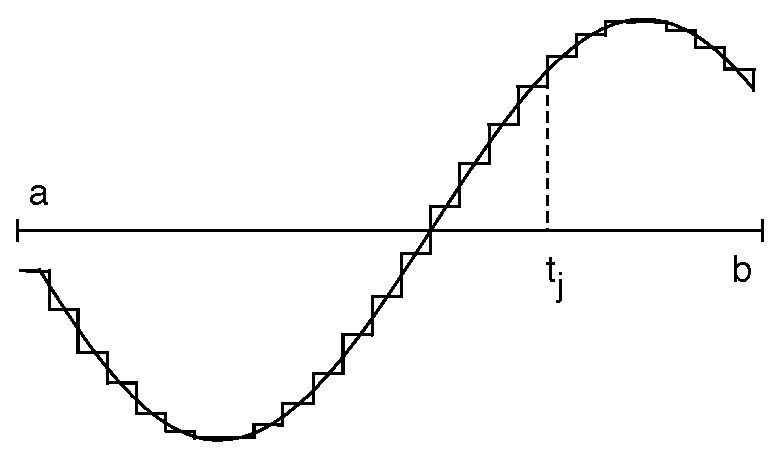
\includegraphics[width=0.5\textwidth]{figures/r/function-approximation}
	\caption{连续函数由其离散化形式来近似,这种离散化将一个函数表示为多个“常数函数”的线性组合,如果将这些“常数函数”看做基,则函数被转化为一个向量}
	\label{f:r-function-approximation}
\end{figure}

以上我们就将一个函数表述为了一种“矢量”形式,当然这里只是一种近似,有了这种矢量形式,我们就可以按照式\ref{e:r-inner-product}计算$L^{2}$中两个函数的内积,假设函数$f$和$g$是两个$L^{2}[0,1]$中的信号,并分别别离散化为$f_N$和$g_N$,其内积为:

\begin{equation}
	\langle f_N,g_N\rangle_{\mathcal{R}^{N}}=\sum^{N}_{j=1}f(t_j)g(t_j)=\sum^{N}_{j=1}f(j/N)g(j/N)
\end{equation}

\noindent 由于函数在$[0,1]$上是连续的,则我们可以将上述的和式转换为积分形式,这给出了$L^{2}([a,b])$上的$L^{2}$内积定义:

\begin{equation}\label{e:r-l2-inner-product}
\begin{aligned}
	\langle f,g\rangle_{L^{2}}=\int^{b}_a f(t)g(t){\rm d}t, && f,g\in L^{2}([a,b])
\end{aligned}
\end{equation}

总结一下以上提供了哪些有用的信息。首先我们对一个$[a,b]$上的连续函数$f(t)$执行离散化使其可以近似为一个“向量”的形式,如图\ref{f:r-function-approximation}所示,理论上,函数是一个无限维的向量,即$N=\infty$,然而在一定的情况下,例如在可接受的误差范围,或者目标函数分布比较平坦(例如本章讨论的间接漫反射光照分布),这种离散化的近似为我们提供了一种高效的计算方法,这种方法说明我们可以用有限维来近似无限维的函数,我们接下来具体讨论这种近似技术相关的一些内容。




\paragraph{正交投影与近似技术}
在图\ref{f:r-function-approximation}中,各个离散的值$f(j/N)$可以看成一个常数函数,它可以通过在原函数$f(t)$上各个固定间隔范围内放置一个矩形函数(box function)来获得,每个矩形函数都是原函数局部区域内的一个近似。这个矩形函数也可以换成其他函数,这给我们一个思路,我们可以使用一些基本函数来近似一个目标函数,这些基本函数的个数是有限的,这构成一个有限维度的函数基,而这种将一个目标函数近似表述在该有限维度的函数基构成的空间上的方法称为投影,我们的目标是要找出怎样的投影才能使投影后的函数(即近似函数)与原函数更加接近,例如每个基函数的系数应该是多少。

假设$V$是向量$\mathbf{v}$(例如它也可以表示函数$f(t)$)所属的无限维空间,现在我们已知一个$N$维的包含正交基$\{\mathbf{e}_i,\cdots,\mathbf{e}_N\}$的子空间$V_0\subset V$,我们的目标是要在$V_0$中寻找一个向量$\mathbf{v}_0$,使其能够最好的近似$\mathbf{v}$。

假设$\mathbf{v}\in V_0$,则$\mathbf{v}$可以是正交基$\{\mathbf{e}_i,\cdots,\mathbf{e}_N\}$的线性张成,我们可以直接按照式\ref{e:r-basis-expand}使用该正交基进行展开,并通过式\ref{e:r-coefficients}计算各个基函数的系数$a_j$;然而如果$\mathbf{v}\notin V_0$,则$\mathbf{v}$不是正交基$\{\mathbf{e}_i,\cdots,\mathbf{e}_N\}$的线性张成,我们无法直接得到$a_j$的解,以下的内容就是聚焦于怎样求解这种近似情况下的系数$a_j$。

假设$\mathbf{v}_0$是$V_0$内对$\mathbf{v}$的一个近似,由于$\mathbf{v}_0\neq\mathbf{v}$,因此它们之间存在一个差值$\mathbf{v}_0-\mathbf{v}$,这称为残差(residual)\mathindex{残差}{residual},我们的目标是需要寻找具有最小残差值的$\mathbf{v}_0$,即:

\begin{equation}
	||\mathbf{v}-\mathbf{v}_0||=\min_{\mathbf{w}\in V_0}||\mathbf{v}-\mathbf{w}||
\end{equation}

根据伽辽金法(Galerkin method)\cite{a:FiniteElementMethodsforGlobalIllumination,a:GalerkinaRadiosity:AHigherOrderSolutionMethodforGlobalIllumination},对最接近与$\mathbf{v}$的$\mathbf{v}_0$的选择应该使得$\mathbf{v}-\mathbf{v}_0$与$V_0$正交,这种方法得到的$\mathbf{v}$在$V_0$中的近似称为正交投影(orthogonal projection)\mathindex{正交投影}{orthogonal projection}。如图\ref{f:r-projection}所示,这里$V$是一个2维空间,矢量$\mathbf{v}\in V$(黑线)在1维空间$V_0$(红线)上的正交投影为$\mathbf{v}_0$,由几何关系可以看出只有当残差矢量$\mathbf{v}_1=\mathbf{v}-\mathbf{v}_0$(蓝色虚线)与$V_0$正交(垂直)时,$\mathbf{v}_0$与$\mathbf{v}$最接近。

\begin{figure}
	\sidecaption
	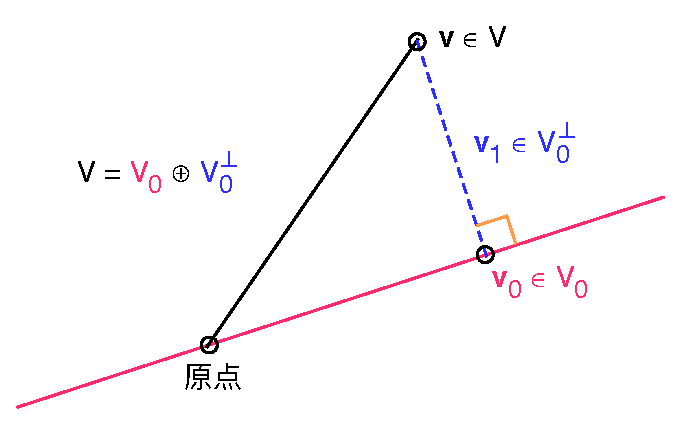
\includegraphics[width=0.51\textwidth]{figures/r/projection}
	\caption{$\mathbf{v}$在$V_0$上的正交投影,$\mathbf{v}$在$V_0$正交投影得到的矢量可以看做是在$V_0$上对$\mathbf{v}$最好的近似,因为其残差$\mathbf{v}_1=\mathbf{v}-\mathbf{v}_0$具有最小的值}
	\label{f:r-projection}
\end{figure}

根据正交的定义可知,$\mathbf{v}-\mathbf{v}_0$与$V_0$中的每个矢量都相交,例如在图\ref{f:r-projection}中,$V_0$中的所有矢量都位于红线上,而所有矢量$\mathbf{v}$相对于$V_0$的残差矢量$\mathbf{v}_1$(如蓝色虚线所示)都垂直于红线。对于残差矢量$\mathbf{v}_1$所在的空间,它有一个特殊的名字,称为$V_0$的正交补(orthogonal complement)\mathindex{正交补}{orthogonal complement},记为$V^{\perp}_0$,它表示$V$上所有与$V_0$正交的矢量集合,即:

\begin{equation}\label{e:r-orthogonal-complement-1}
	V^{\perp}_0=\{\mathbf{v}\in V;\langle\mathbf{v},\mathbf{w}\rangle=0,\mathbf{w}\in V_0\}	
\end{equation}

\noindent 可以看出,$V$中的每个矢量都可以唯一看做是$V_0$中的一个矢量与$V^{\perp}_0$中一个矢量的和,即$\mathbf{v}=\mathbf{v}+\mathbf{v}_1$,因此有:

\begin{equation}\label{e:r-orthogonal-complement-2}
	V=V_0\oplus V^{\perp}_0
\end{equation}

\noindent 其中,符号$\oplus$表示$V_0$和$V^{\perp}_0$相互正交,正交补的概念在我们后面介绍小波分析的时候非常重要。

那么怎样求解正交投影$\mathbf{v}_0$的各个系数$a_j$呢?根据上述正交投影的定义,即需要求解满足$\mathbf{v}-\mathbf{v}_0$与任意矢量$\mathbf{w}\in V_0$正交的条件。因为$\mathbf{e}_1,\cdots,\mathbf{e}_N$是$V_0$的一个基,所以只需要表明$\mathbf{v}-\mathbf{v}_0$与每个$\mathbf{e}_k,k=1,\cdots,N$正交,令$\mathbf{v}_0=\sum^{N}_{j=1}a_j\mathbf{e}_j$,则:

\begin{equation}
	\langle\mathbf{v}-\mathbf{v}_0,\mathbf{e}_k\rangle=\langle\mathbf{v}-\sum^{N}_{j=1}a_j\mathbf{e}_j,\mathbf{e}_k\rangle
\end{equation}

\noindent 因为$\mathbf{e}_1,\cdots,\mathbf{e}_N$是相互正交的,所以上式中仅有的非零项是当$j=k$时,即:

\begin{equation}
\begin{aligned}
	\langle\mathbf{v}-\mathbf{v}_0,\mathbf{e}_k\rangle&=\langle\mathbf{v},\mathbf{e}_k\rangle-a_k\langle\mathbf{e}_k,\mathbf{e}_k\rangle\\
	&=\langle\mathbf{v},\mathbf{e}_k\rangle-a_k\\
	&=0
\end{aligned}
\end{equation}

\noindent 从而可以得出$a_j=\langle\mathbf{v},\mathbf{e}_j\rangle$。




\subsubsection{小波分析基础}\label{sec:r-wavelets}
上面的正交投影提供了一种使用一组已知的函数基来近似一个目标函数的方法,这在数学中非常有用,因为这些基函数的系数反应这原函数不同的信息,例如对于每个在$a$处无限可导的实或者复函数函数$f(x)$都可以在$a$处展开为泰勒级数$\sum^{\infty}_{n=0} \cfrac{f^{(n)}(a)}{n!}(x-a)^{n}$,它代表着函数$f(x)$在$a$领域内的近似,越高阶的项对近似函数的贡献越小,所以通常我们可以舍弃高阶项并可以(根据需求)得到很好的近似;另外对于前面介绍的傅里叶分析,一个可积的函数可以转换为无数个正弦和余弦函数,而这些正余弦函数代表着不同的频率,因此形成一个函数的频率分布,然后我们可以通过(根据需要)设置较高频率的正余弦函数的系数为0来实现降噪处理,如图\ref{f:r-fourier}所示,通过舍弃高频的分量,原函数仍然可以被很好的近似。

\begin{figure}
\begin{fullwidth}
	\begin{subfigure}[b]{0.5\thewidth}
		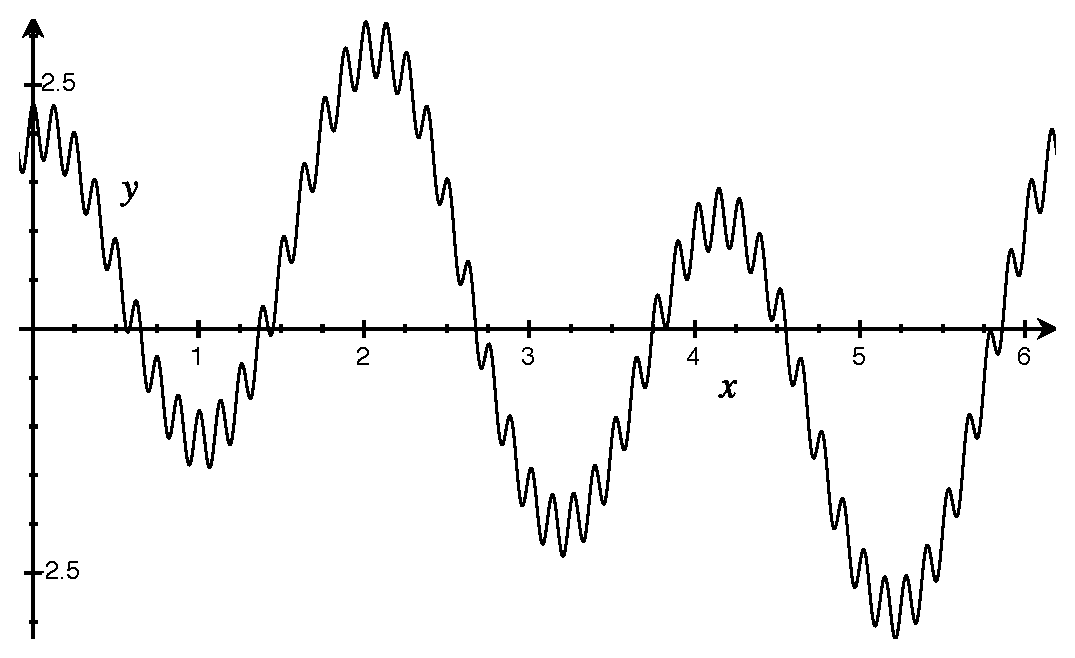
\includegraphics[width=1.0\textwidth]{figures/r/fourier-1}
		\caption{$f(t)=\sin (t)+2\cos(3t)+0.3\sin(50t)$}
	\end{subfigure}
	\begin{subfigure}[b]{0.5\thewidth}
		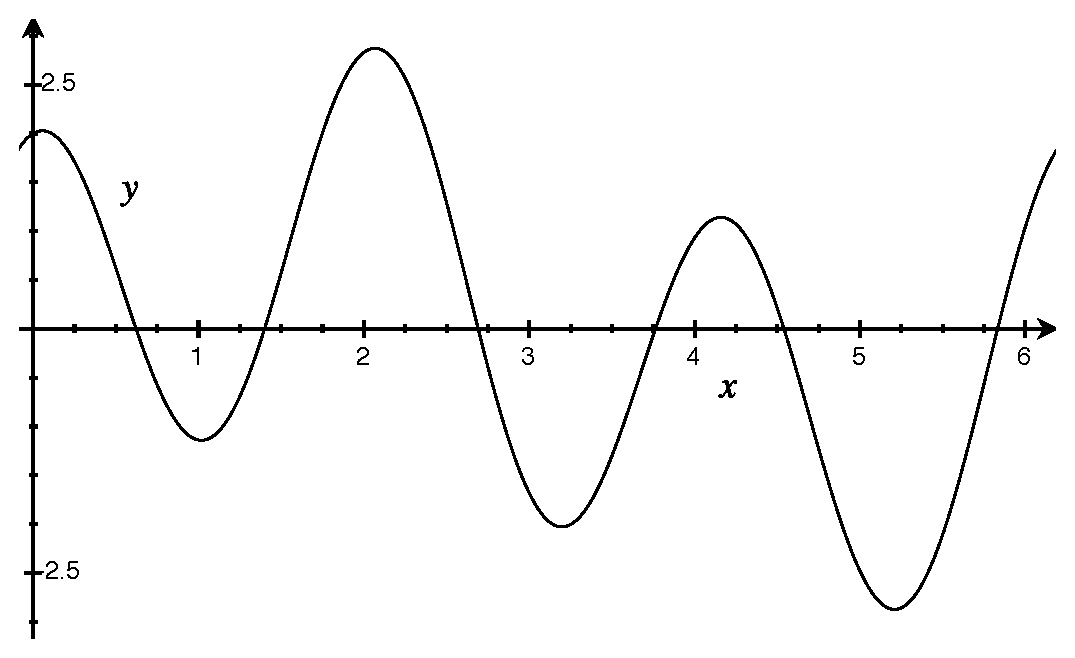
\includegraphics[width=1.0\textwidth]{figures/r/fourier-2}
		\caption{$f(t)=\sin (t)+2\cos(3t)$}
	\end{subfigure}
	\caption{一个函数被表述为一系列正余弦函数的线性组合,这些正余弦函数代表了不同的振荡频率,通过消除高频的函数项($0.3\sin(50t)$),可以实现噪声消除,例如(a)中的高频项可能是录音磁带中嘶嘶的背景声,通过消除高频的噪声,原函数的主要特征仍然可以被很好地近似(b)}
	\label{f:r-fourier}
\end{fullwidth}
\end{figure}

除了消除噪声,信号分析中的另一个相关问题是数据压缩,由于目标函数可以分解为多个基函数的线性组合,因此我们需要保存这些基函数的系数,这些系数的数量可能非常大,例如本章讨论的辐射度方法其实就是将辐射度展开为$n$个常数函数的线性组合,每个常数函数对应于一个曲面,因此总共需要存储$n^{2}$个形状系数,而实际上,形状系数的分布非常稀疏,在一定的容错范围内,我们可以忽略掉那些系数非常小的项,以减少数据的存储以及后续线性方程求解的复杂度。

上述两个问题理论上都可以通过傅里叶分析来解决,然而尽管如此,傅里叶分析还是具有缺点,最大的缺点是它的基函数是无始无终的周期性正弦波和余弦波,因此该方法适合处理那些(过滤或压缩)那些具有近似周期性的波动信号,例如图\ref{f:r-fourier}中的信号,而对于那些具有显著局部特征的信号,正弦波和余弦波就无能为力了。例如\ref{f:r-wavelet}(a)所示的信号,它表示一段声音信号,其包含两个噪声尖峰需要去掉,由于这种局部尖峰不具有周期性,所以无法使用正余弦波进行分解。

为了分析这种信号的局部特征,小波(wavelet)\mathindex{小波}{wavelet}被提出,与无限循环的正余弦波不一样,小波通常仅持续几个周期,即它仅仅在一段有限的区间内有非零值,例如\ref{f:r-wavelet}(b)所示,我们称这种特征为紧支撑(compact support)\mathindex{紧支撑}{compact support}(当然也有小波函数不是紧支撑的,但这类小波函数通常仅在有限区间内具有显著的值,其他大部分区域则逐渐收敛到0),小波的这种特征使得它可以表述信号局部区域的信息。小波可以沿时间轴前后平移,也可以按比例伸展和压缩以获取低频和高频小波,这样构造好的小波函数也可以像傅里叶级数那样用于滤波或压缩信号,同时能够很好地辨识信号的局部特征。

\begin{figure}
	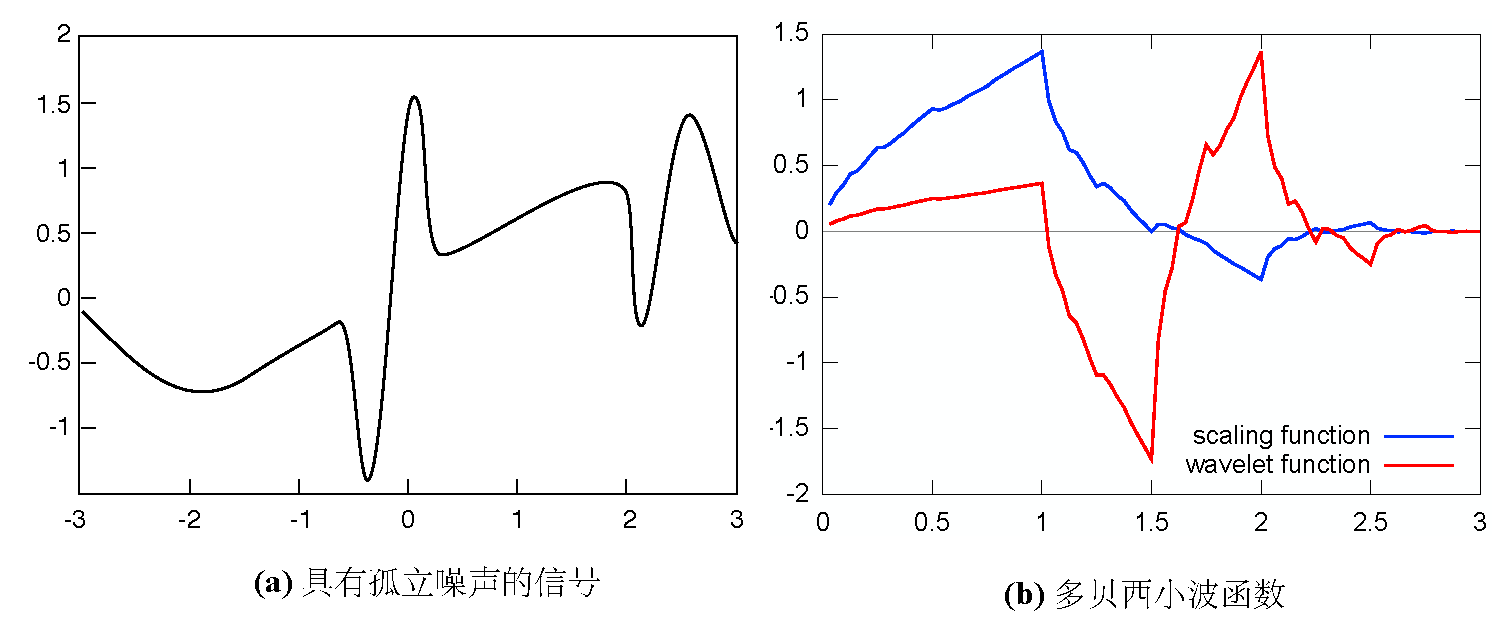
\includegraphics[width=1.0\textwidth]{figures/r/wavelet}
	\caption{信号有时具有比较显著的局部噪声(a),由于这种噪声不具备周期性,因此不能使用傅里叶变换进行处理,小波是一类紧支撑的函数(b),它们仅在局部一段有限的空间内有非零值,所以非常擅长处理这种信号的局部特征}
	\label{f:r-wavelet}
\end{figure}

为了实现把一个信号分解展开的有效算法,这些算法的基函数必须满足正交性,对于傅里叶变换,正余弦都具有比较好的正交性,例如对于正弦函数:

\begin{equation}
	 \cfrac{1}{\pi}\int^{2\pi}_0 \sin(nt)\sin(mt)=\begin{cases}
		0 & \text{若} n\neq m\\
		1 & \text{若} n = m
	\end{cases}
\end{equation}

然而对于小波函数,要使平移和伸缩之后的小波仍然满足正交性则非常困难,因此怎样构造相互正交的小波函数基,以及怎样高效计算小波基函数的系数都是小波分析中比较重要的内容。以下我们首先通过构造最简单的小波函数基--哈尔小波以介绍小波函数基的基本构造方法及其相关的一些概念,并以此引出小波分析中的多分辨率分析的概念。




\subsubsection{哈尔小波}\label{sec:r-haar-wavelet}
虽然小波是由一些紧支撑(在有限空间具有非零值)的基函数构成,但是这些基函数并不是任意的,例如它需要能够反应函数不同的频率分布,同时还需要满足基函数之间的正交性,为此小波基函数使用一种特殊的方式构造而成,本节以哈尔小波为例讨论小波基函数的基本构造思路,其他小波的构造则是类似的。

小波的基函数由两个非常重要的函数构成,即尺度函数(scaling function)\mathindex{尺度函数}{scaling function}$\phi$和小波函数(wavelet function)\mathindex{小波函数}{wavelet function}$\psi$,这两个函数产生了一组可以用于分解和重构信号的函数簇。

哈尔尺度函数定义为(如图\ref{f:r-haar-functions}(a)所示):

\begin{equation}
	\phi(x)=\begin{cases}
		1 & \text{ 如果 } 0\leq x<1\\
		0 & \text{ 其他 }
	\end{cases}
\end{equation}

\noindent 通过对上述位于位置0处的哈尔尺度函数执行平移操作,形成了一个具有相同尺度(即相同长度的非零值区域)的函数集,由于这些尺度函数都是相互正交的(因为$\phi(x-j)$与$\phi(x-k)$的支撑集不相交),这构成一个函数空间,令$V_0$为所有形如:

\begin{equation}
	\sum_{k\in \mathcal{Z}}a_k\phi(x-k),a_k\in \mathcal{R}
\end{equation}

\noindent 组成的函数空间,这里$k$为一有限内的整数,直接使用它们来分解一个函数其实就得到类似图\ref{f:r-function-approximation}的结果。

\begin{figure}
	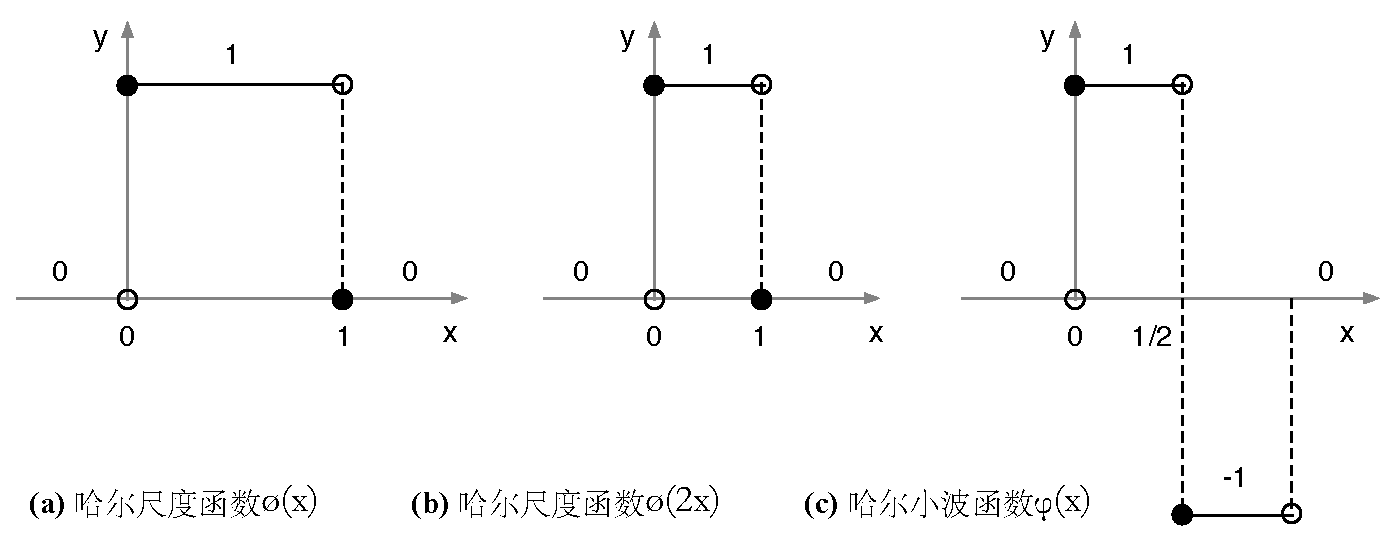
\includegraphics[width=1.0\textwidth]{figures/r/haar-functions}
	\caption{哈尔尺度函数及哈尔小波函数构成哈尔小波的两个基础构造块,小波的尺度函数可以按分辨率逐层分解,例如(a)被分解为两个更高分辨率的(b)和(c)的组合,更高分辨率的尺度函数可以表述更精细的局部信息,小波函数构造块的这种特殊构造方式使得不同分辨率之间的函数构造块也是相互正交的}
	\label{f:r-haar-functions}
\end{figure}

为了能够捕捉高频信号,我们需要更窄的尺度函数,因为高频信号往往在更小的范围内有很大的变化,由此可以取$\phi$的一半宽度形成一个更窄的尺度函数$\phi(2x)$,如图\ref{f:r-haar-functions}(b)所示。同样对该尺度函数执行平移操作,得到一个形如:

\begin{equation}
	\sum_{k\in \mathcal{Z}}a_k\phi(2x-k),a_k\in \mathcal{R}
\end{equation}

\noindent 组成的$V_1$函数空间,与$V_0$中的尺度函数不同的是,由于$\phi(2x-k)=\phi(2(x-k/2))$,所以这里的平移尺度为$k/2$个单位。以此类推可以得到$j$级阶梯函数空间$V_j$,它是由以下函数集构成:

\begin{equation}
	\{\cdots,\phi(2^{j}x+1),\phi(2^{j}x),\phi(2^{j}-1),\phi(2^{j}+1),\cdots\}
\end{equation}

\noindent 注意,虽然每个阶梯空间$V_j$内的尺度函数都是相互正交的,但是到目前为止我们并没有称其为该空间内的正交基,这是因为正交基中的每个基函数$\mathbf{e}_i$必须满足$||\mathbf{e}_i||=1$,而因为$\int^{\infty}_{-\infty}(\phi(2^{j}x))^{2}{\rm d}x=1/2^{j}$,所以这些尺度函数还应该除于这个系数,才能成为$V_j$的标准正交基:

\begin{equation}
	\{2^{j/2}\phi(2^{j}x-k);k\in\mathcal{Z}\}
\end{equation}

\noindent 显然$V_j$是紧支撑的分段常数函数空间,其间断点在下列集合中:

\begin{equation}
	\{\cdots,-1/2^{j},0,1/2^{j},2/2^{j},3/2^{j},\cdots\}
\end{equation}

\noindent 上述的这种按频率对尺度函数的划分产生了一个很有趣的结果,即:

\begin{equation}\label{e:r-multiresolution-relationship}
	V_0\subset V_i\subset\cdots V_{j-1}\subset V_j\subset V_{j+1}\cdots
\end{equation}

\noindent 上述的关系可以通过图\ref{f:r-v-j}的集合关系理解,这样的结果并不让人惊讶,因为每个$V_j$中的基函数被分解为$V_{j+1}$中两个相邻基函数的和,只需要将对应的系数分配到这两个加数基函数上即可。由于$V_j$表示的是函数空间,即意味着所有能用$V_j$中的函数基分解的函数也一定能够被$V_{j+1}$中的函数基分解,因此随着分辨率的提高,不会损失任何信息。式\ref{e:r-multiresolution-relationship}的这种关系也说明了为什么$V_j$是以$\phi(2^{j}x)$而不是其他方式进行细分。

\begin{figure}
	\begin{fullwidth}
		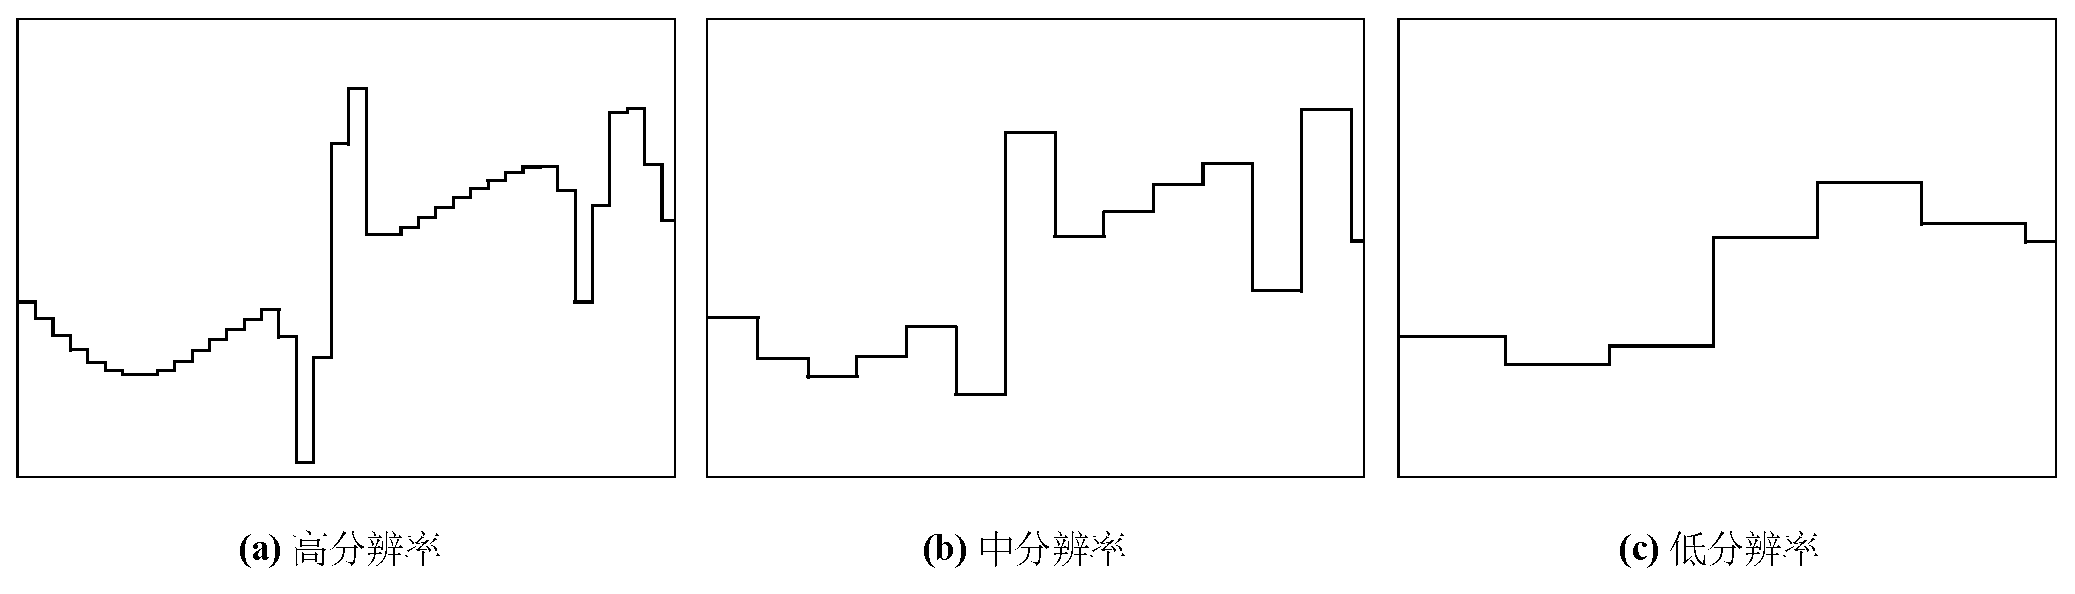
\includegraphics[width=1.0\thewidth]{figures/r/scalings}
		\caption{以不同分辨率的哈尔尺度函数对图\ref{f:r-wavelet}(a)中的信号进行近似,较平坦的区域可以使用较低分辨率的哈尔尺度函数进行近似,这可以使用更少的系数,但是频率变化较大的区域则需要很高分辨率的尺度函数才能很好地近似}
		\label{f:r-scalings}
	\end{fullwidth}
\end{figure}

图\ref{f:r-scalings}显式了使用不同分辨率下的哈尔尺度函数对图\ref{f:r-wavelet}(a)中的信号的近似,可以看出低分辨率的尺度函数能够很好地近似函数中较平坦的部分,如图\ref{f:r-scalings}(c)所示,使用低分辨率尺度函数的好处是可以大大减少基函数系数的数量;然而局部频率变化比较大的区域则需要较高分辨率的尺度函数才能捕捉,如图\ref{f:r-scalings}(a)所示。

理想情况下,为了节省基函数系数的数量,我们希望对于平坦的部分使用较低分辨率的尺度函数,而仅对高频部分使用高分辨率的尺度函数。然而目前已有的知识并不能做大如此,因为各个分辨率下的尺度函数集构成的基函数并不是相互正交的,我们仅能使用一种特定的分辨率对函数进行近似,而没办法将它们“组合”起来,这其实有点类似于经典辐射度方法按照固定的分辨率对场景中的曲面进行划分,我们仅能选择使用的分辨率的大小,而不能根据辐射度的分布特征对不同区域的曲面使用不同的分辨率。此外,我们无法实现对高频噪声的滤除(考虑图\ref{f:r-scalings}(a),虽然我们捕捉到了高频部分,但是怎么将其噪声滤除掉呢?)。

为此,小波分析引入了另外一个小波函数$\psi$,它能将各个不同分辨率的尺度函数组合起来,并且能够孤立出噪声以实现噪声滤除。




\paragraph{哈尔小波函数}
既然$V_j$是$V_{j+1}$的子集(式\ref{e:r-multiresolution-relationship}),那么能不能把$V_{j+1}$中的$V_j$部分分解出来呢,然后剩下的部分存在于($V_j$相对于$V_{j+1}$的)正交补$V^{\perp}_j$中,如图\ref{f:r-v-j}中的灰色部分,该正交补保留了第$j+1$级分辨率的特征,它可以有效地表述噪声部分,小波函数$\psi$的出现就是为了实现将$V_{j+1}$分解成$V_j$和正交补$V^{\perp}_j$。

\begin{figure}
	\sidecaption
	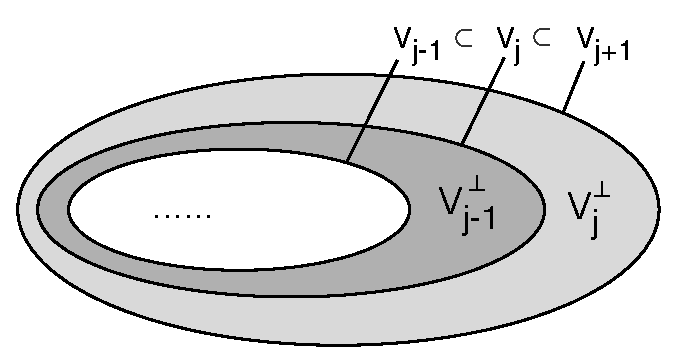
\includegraphics[width=0.5\textwidth]{figures/r/v-j}
	\caption{多级分辨率的尺度函数空间形成了一个嵌套的关系,我们需要找出能够表述每一级正交补空间的基函数,这样才能对高频的噪声进行滤除,它们存在于这些正交补当中;同时还能将所以尺度函数空间组合起来}
	\label{f:r-v-j}
\end{figure}

由于$V_{j+1}$中的尺度函数和$V_j$中的尺度函数不是正交的,因此无法直接用$V_{j+1}$中的尺度函数减去$V_j$中的尺度函数来表述其正交补,我们需要定义另外一个函数$\psi$来表述正交补中的基函数。以下我们以$V_0$为例讨论其正交补$V^{\perp}_0$中的基函数,然后将其推广到$V_j$。

我们的目标是要将$V_1$分解为由哈尔尺度函数$\phi$表述的$V_0$,以及由$\psi$表述的正交补$V^{\perp}_0$。由于$V_0$是由$\phi$及其平移系构成,因此我们有理由期望$V_0$的正交补也是由小波函数$\psi$及其平移系构成。以下两点条件有助于我们构造合适的小波函数$\psi$:

\begin{enumerate}
	\item $\psi$是$V_1$的成员,所以可以表示为$\psi(x)=\sum_{l}a_l\phi(2x-l),a_l\in\mathcal{R}$,这里仅有有限个$a_l$是非零值(实际上所有位于$V_0$中的那些尺度函数对应的系数都是0),即$\psi$是$V_1$中某部分尺度函数的线性组合。
	\item $\psi$与$V_0$正交,即$\int\psi(x)\phi(x-k){\rm d}x=0$对所有整数$k$成立,这是正交补概念的要求(式\ref{e:r-orthogonal-complement-1}和式\ref{e:r-orthogonal-complement-2})。
\end{enumerate}

所有满足上述条件的函数都可以用作小波函数$\psi$,哈尔小波中($V^{\perp}_0$)使用的小波函数定义如下:

\begin{equation}
	\psi(x)=\phi(2x)-\phi(2x-1)
\end{equation}

\noindent 即是直接取$V_1$相邻两个尺度函数的差值,如图\ref{f:r-wavelet}(c)所示。

将此小波函数的构造方法推广到各个阶梯就能够得出所有阶梯的正交补,以下我们称正交补$V^{\perp}_j$为$W_j$,由上述的分解方法可知,$W_j$是由形如:

\begin{equation}
	\sum_{k\in\mathcal{Z}}a_k\psi(2^{j}x-k);a_k\in\mathbf{R}
\end{equation}

\noindent 构成的函数空间。对整个阶梯的函数空间进行分解,则无限空间$L^{2}$可以被分解为无限个正交直和(如图\ref{f:r-v-j}所示):

\begin{equation}\label{e:r-wavelet-decompose-1}
	L^{2}(\mathcal{R})=V_0\oplus W_0\oplus W_1\oplus\cdots
\end{equation}

\noindent 所有对任何$f\in L^{2}(\mathcal{R})$可以唯一地写成:

\begin{equation}\label{e:r-wavelet-decompose-2}
	f=f_0+\sum^{\infty}_{j=0}w_j
\end{equation}

\noindent 其中,$f_0\in V_0$,$w_j\in W_0$。

图\ref{f:r-decompose}展示了某一级空间$V_{j+1}$中的函数分解,其中橙色线段的常数函数位于$V_j$中,而灰色部分则位于正交补$W_j$中,可以看到通过这种方式可以把噪声尖峰部分分解出来。只要使用足够高分辨率的函数空间$V_j$对函数进行近似,就可以滤除指定宽度范围内的尖峰噪声。此外,尺度函数空间的分解使各个阶梯的尺度函数可以组合起来,在一些平坦的部分可以使用更低分辨率的尺度函数进行表述,大大减少了基函数系数的数量。

\begin{figure}
	\sidecaption
	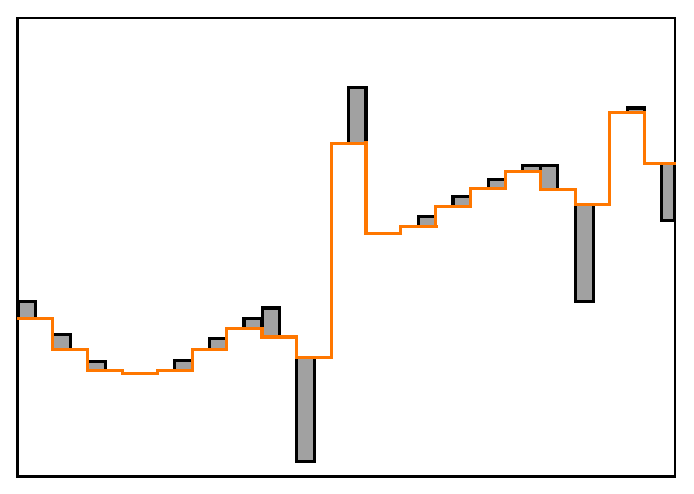
\includegraphics[width=0.5\textwidth]{figures/r/decompose}
	\caption{对图\ref{f:r-function-approximation}(a)中的信号按某个分辨率的尺度函数空间$V_{j+1}$进行近似,然后将其分解为到$V_j$(橙色线条)和$W_j$(灰色区域)空间中,这种分解形成了小波分析的重要基础}
	\label{f:r-decompose}
\end{figure}

以上,我们介绍了小波分析的所有基础知识,下面我们再对其运用过程进行总计,这包括怎样对$V_j$进行分解,以及怎样将处理过的信号进行重建。





\paragraph{分解和重构}
为了对信号进行处理,需要首先对信号进行分解,这涉及将信号函数分解到$V_0$空间以及各个分辨率阶梯对应的正交补$W_j$中,如式\ref{e:r-wavelet-decompose-1}和式\ref{e:r-wavelet-decompose-1};然后对信号进行处理,例如去掉高分辨率尖峰项$w_j$(噪声滤除),或者去掉某些值非常小的系数(数据压缩);最后对处理后的信号进行重构还原原始信号。

由于高阶梯尺度函数空间保持低阶梯尺度函数空间极其正交补,所以分解过程首先涉及将函数投影到某个足够高分辨率的尺度函数空间,然后再进行逐级分级,即原始信号函数被近似为:

\begin{equation}
	f_j(x)=\sum_{l\in\mathcal{Z}}a_l\phi(2^{j}x-1)
\end{equation}

\noindent 这里可以直接对信号在$x=\cdots,-1/2^{j},0,1/2^{j},\cdots$处取样,从而得到系数$a_l=f(l/2^{j})$的值(对于其他小波尺度函数,则可以使用前面讲述的正交投影方法,通过计算函数与各个基函数的内积来得到该基函数对应的系数)。该正交投影的过程得到一个近似的阶梯函数,例如图\ref{f:r-function-approximation}和\ref{f:r-wavelet}(a)所示等。

接下来是把$\phi(2^{j}x-l)$分解为各个$W_l(l<j)$的分量。根据前面小波函数$\psi$的构造方式,我们很容易得到相邻两阶尺度函数和小波函数之间的关系,例如第$j-1$级的尺度函数和小波函数可由第$j$级的尺度函数线性组合而成(这里只说明每阶中第0和1个索引位置处的函数):

\begin{equation}\label{e:r-harr-decompose}
	\begin{aligned}
		\phi_{j-1,0}&=\phi_{j,0}+\phi_{j,1}\\
		\psi_{j-1,0}&=\phi_{j,0}-\phi_{j,1}
	\end{aligned}
\end{equation}

\noindent 上述的关系可以用于上$j$阶向第$j-1$阶的分解。反过来,也可以对上式方程组进行变换,得到第$j$阶的尺度函数关于第$j-1$阶尺度函数和小波函数的线性组合:

\begin{equation}\label{e:r-harr-reconstruction}
\begin{aligned}
	\phi_{j,0}&= \cfrac{1}{2}\phi_{j-1,0}- \cfrac{1}{2}\psi_{j-1,0}\\
	\phi_{j,1}&= \cfrac{1}{2}\phi_{j-1,0}+ \cfrac{1}{2}\psi_{j-1,0}
\end{aligned}
\end{equation}

\noindent 上式可以用于从低阶向高阶尺度函数的重建过程。根据类似的关系可以直接推导出一个直接的分解和重构公式,这里仅关注小波分析的基本思路,更详细的过程可以参见\cite{b:AFirstCourseinWaveletswithFourierAnalysis,b:AnIntroductiontoWavelets}等资料。




\paragraph{多分辨率分析}
以上我们通过哈尔小波为例介绍了小波分析的基本思路和原理,本节最后我们进一步对上述这些内容进行更系统的梳理。

本节开头介绍了怎样将函数表示为一个向量,这即是通过将函数正交投射到一个由一些基函数构成的函数空间,这样目标函数被表述为这些基函数的线性组合,每个基函数对应的系数由目标函数与该基函数的内积决定,这些系数构成了目标函数在该函数空间中的一个向量;如果函数空间的维度(即基函数的数量)是无限的,例如$L^{2}$空间,则目标函数可以被精确表述(如傅里叶变换),通常我们只能用有限维度的函数空间来近似一个函数。

基函数的定义域可以是无限的,例如傅里叶变换中的正余弦函数,这样的基函数可以提取目标函数的一些全局(周期)性特征,本章我们对紧支撑的基函数更感兴趣,因为紧支撑的基函数通常只在非常小的范围内取非零值,因此能够提取目标函数的局部(频率变化)信息。

紧支撑的基函数通常都是有规律的一个函数集,例如通常对某个简单的函数$h$执行平移或缩放形成$L^{2}$上的一个函数基。由于基函数是紧支撑的,目标函数局部表述的精确度取决于基函数的近似能力,例如常数函数的近似效果是最差的,因此通常需要更高的分辨率才能对目标函数有较好的近似,但是其基函数系数的计算则特别简单,这只需要对目标函数上某个位置处的值进行取样即可;另一些基函数使用高阶的多项式,这样的基函数对目标函数的局部分布有较强的近似能力,因此只需要较低的分辨率(即更少的基函数数量)即可对目标函数有较好的近似,但是其基函数的系数计算则相对复杂,因为这需要求目标函数和每个基函数的内积值。

我们上述讨论的函数基都是某个单一函数构成的函数集,即它们的形式和尺度都是相同的,如果目标函数比较简单,则选取一个合适的分辨率(或者尺度)即可;然而对于复杂的目标函数,其分布非常不规律,为了覆盖一些精细的局部信息,这需要使用非常高的分辨率,然而这种高分辨率的尺度对大部分平坦区域又是浪费的。因此人们提出了多分辨率分析(multiresolution analysis)\mathindex{多分辨率分析}{multiresolution analysis}方法,又称为多尺度近似(multiscale approximation)\mathindex{多尺度近似}{multiscale approximation},该方法主要和小波分析有关,即基函数是由多个尺度的函数集构成,这些不同尺度函数集的关系满足式\ref{e:r-multiresolution-relationship},而通过巧妙的构造,这些上下级几何之间的正交补可以由一个小波函数集构成,该小波函数集可以直接由对应的尺度函数导出(如式\ref{e:r-wavelet-decompose-1}和式\ref{e:r-wavelet-decompose-2})。通过多分辨率分析,目标函数被分解为一个低分辨率的近似$f_0$以及各个正交补空间的近似$w_j$的和(如式\ref{e:r-orthogonal-complement-2})。

当目标函数由$V_j$向$V_{j-1}$和$W_{j-1}$进行分解时,函数$f_j$被分解为$f_{j-1}+w_{j-1}$,其中$f_{j-1}$是那些更平坦的区域可以使用更少的系数(因为使用了更大尺度的尺度函数)进行存储,而$w_j$又保留了函数高频部分的细节,由于$f_{j-1}$是$\phi_{j-1}$对应的尺度函数集的线性组合,因此尺度函数$\phi(x)$又称为平滑函数(smooth function)\mathindex{平滑函数}{smooth function},而$w_{j-1}$是$\psi_{j-1}(x)$中对应小波函数集的线性组合,因此小波函数$\psi(x)$又称为细节函数(detail function)\mathindex{细节函数}{detail function}。

由于$W_{j-1}$中的小波函数与$V_j$中的基函数尺度是相同的,因此分解到$W_{j-1}$中的部分并没有减少正交投影系数的数量,但是由于$V_{j-1}$中的尺度函数相较$V_j$有更小的尺度,因此这种转变可以减少系数的数量,但是这种系数的较少取决于目标函数局部区域的平坦性,例如对于局部区域几乎为常数的函数,当分解到更低分辨率的尺度函数上时,此时的正交补中基函数的系数将小到几乎为0,所以可以直接忽略掉。

上述的推导引出了一个度量小波的重要属性,即消失矩(vanishing moments)\mathindex{消失矩}{vanishing moments},如果一个小波函数$\psi(x)$满足以下条件:

\begin{equation}
	\int x^{i} \psi(x){\rm d}x=0,i=0,\cdots,M-1
\end{equation}

\noindent 则称该小波函数具有$M$阶消失矩,消失矩的定义说明小波函数正交于所有小于$M$的低阶多项式。如果一个函数能够很好地被一个低阶($\leq M$)的多项式表述,而该函数正交投影使用的小波函数$\psi$具有$M$阶消失矩,则该级函数的分解后该小波函数对应的系数为0。

小波的消失矩阶数是减少系数数量的关键,对于更平坦的分布函数,我们可以使用具有低阶消失矩的小波,例如哈尔小波,这使得投影系数的计算非常简单;但是对于局部分布比较复杂的目标函数,具有低阶消失矩的小波通常不能有效地减少系数的数量,此时必须使用更复杂的多项式小波函数才能有效地表述局部信息,从而实现系数的减少,但是高阶多项式表述的小波函数的系数计算则非常复杂。




\subsubsection{小波辐射度方法}\label{sec:r-wavelet-radiosity}
以上实际上我们已经介绍了小波辐射度方法的基本思路,这和小波在其他领域的一些运用是类似的,例如数字图像处理中的图像压缩或噪声滤除\cite{b:DigitalImageProcessing},由于不同小波相关的数学表述比较复杂,这写内容和知识超出了本书的范围,我们仅对其基本思路进行介绍,感兴趣的读者可以阅读\cite{a:WaveletaRadiosity,a:WaveletMethodsforComputerGraphics,a:WaveletRadiosityonArbitraryPlanarSurfaces,a:RadiosityinFlatland}等进行深入学习。

特别需要注意的是,前面讨论的阶层式辐射度方法其实是小波辐射度方法中的一种特例,即使用哈尔小波作为小波函数基的表述,四叉树的结构类似于尺度函数尺度的缩放,只不过曲面是两个位置变量的函数,而我们以上介绍的只是单变量的小波分解,但是由于两个位置变量彼此是独立的,因此很容易扩展到多变量函数,因此形成一棵四叉树的阶层(多分辨率)结构;此外,在阶层式辐射度方法中根据一定的误差阈值选择保留的形状系数,就相当于小波辐射度方法中根据一定的条件忽略那些高分辨率的小波函数系数。





\subsection{非连续网格化}\label{sec:r-discontinuity-meshing}
到目前为止,本章介绍的所有曲面细分技术都没有考虑可见性的问题,所有曲面仅仅按照几何尺度进行细分。然而由于物体之间存在遮挡关系,因此曲面上会存在非连续的阴影边缘,这种非连续性打破了辐射度方法关于细分曲面内各处辐射度为常数的假设,显然这将导致渲染结果呈现较大的误差。

漫反射曲面上辐射度分布的非连续性主要表现为曲面上的一些边界线(boundary),这些边界线主要是由于物体之间的遮挡关系产生的,例如一个物体的部分重叠于另一个物体之上,或者由于面积光源产生的本影边界(umbra boundary)\myindex{本影边界}{umbra boundary}和半影边界(penumbra boundary)\myindex{半影边界}{penumbra boundary},这些不规则边界将曲面细分为更复杂的不规则曲面,这些更小的细分曲面更接近辐射度方法的假设。因此,如果我们能够找到所有这些非连续的边界线,则可以利用它们来指导对曲面的网格化,这形成非连续网格(discontinuity mesh)\myindex{非连续网格}{discontinuity mesh},相应的技术称为非连续网格化(discontinuity meshing)\myindex{非连续网格化}{discontinuity meshing}技术。

本节的主要内容便是从物体之间的几何遮挡关系提取出所有这些边界线,然后用于指导更精确的曲面细分。然而非连续网格化产生的细分曲面往往是不规则的,这有悖于前面介绍的阶层式辐射度方法中按照规则的尺寸(分辨率)对场景进行划分,我们将在第\ref{sec:r-combine}节介绍一种改进的方法用于组合非连续网格化和阶层式辐射度方法。




\subsubsection{非连续边界}
光照的不连续是指从某个边界开始,光照的分布按一定的方式进行变化,特别地,我们这里主要是指光照随着几何位置的变化(由于物体间的遮挡)而变化。

我们可以将这种不连续的边界线分为三类\cite{a:ADiscontinuityMeshingAlgorithmforAccurateRadiosity}:即$D^{0}$不连续,$D^{1}$不连续和$D^{2}$不连续,其中这里的阶数$0,1$和$2$表示光照变化的阶数,分别对应常数,线性和二次函数变化。

$D^{0}$不连续是指这样的边界,处于它们两边位置内的光照分别为不同的常数,$D^{0}$不连续边界通常是由于遮挡体的某个边位于接受面上,如图\ref{f:r-boundaries}中的AB线段,它同时位于遮挡体和接受面上,所以对于右上角的点光源,位于AB左边的区域内光照值为0(常数),而位于AB右边的区域内的光照值为一个常数光照值。

由$D^{0}$不连续的定义可知,由点光源导致的硬阴影边界也是$D^{0}$不连续的,如图\ref{f:r-boundaries}中$D^{'}A,C^{c}D^{'}$和$C^{'}B$三个边界线均是由点光源产生,它们两边的区域内的光照均为不同的常数值。因此接受面上的区域$D^{'}ABC^{'}$构成一个常数光照值区域,这符合辐射度方法的假设,我们应当把它们特别地细分出来。

\begin{figure}
\sidecaption
	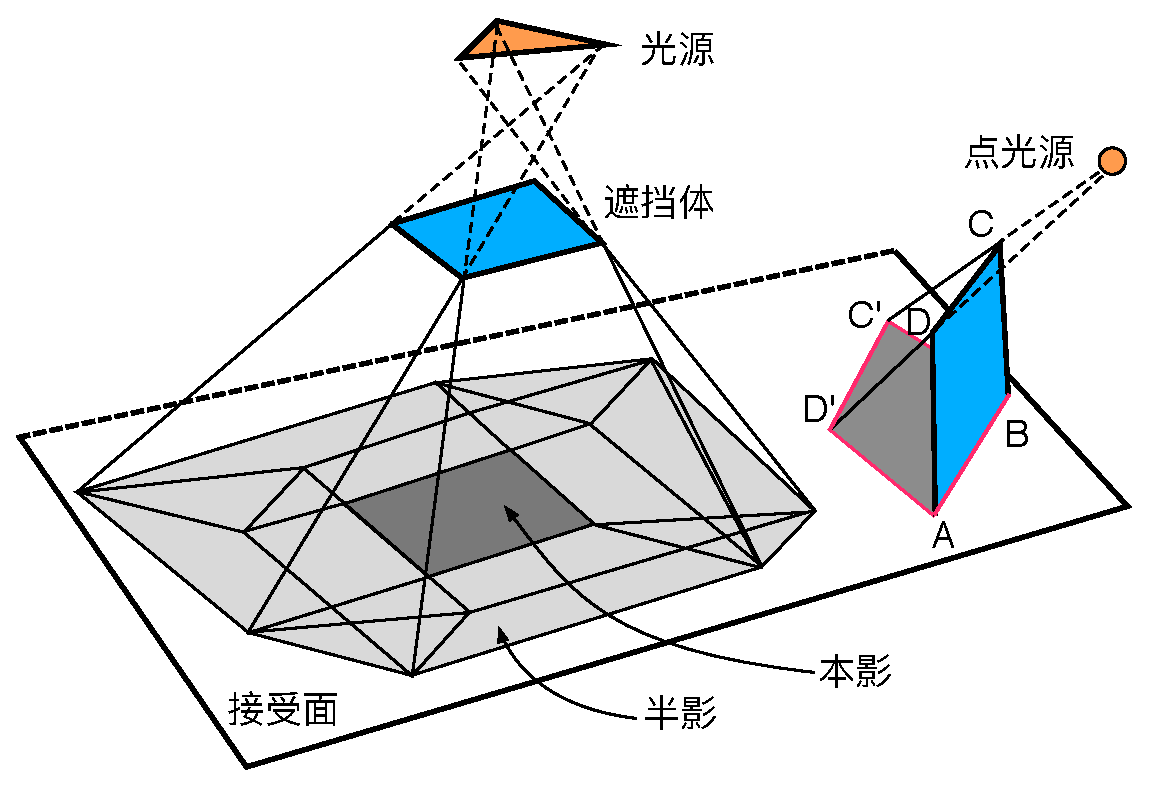
\includegraphics[width=.65\textwidth]{figures/r/boundaries}
	\caption{物体表面由于物体间的遮挡关系造成的光照分布不连续,这些不连续性可以分为$D^{0},D^{1}$和$D^{2}$三类,我们可以提取出所有非连续的边界线,这些边界线将表面划分为多个细分曲面,每个细分曲面的光照值可以按照对应光照的非连续性(常数,线性或二次方)分布进行计算}
	\label{f:r-boundaries}
\end{figure}

$D^{1}$和$D^{2}$不连续是指光照的变化呈一次(线性)和二次变化,它们均是由于面积光源通过遮挡体的边界投影到接受面上而形成,如图\ref{f:r-boundaries}所示,一个三角形的面积光源透过一个矩形遮挡体在接受面上形成多个边界线,其中本影区域内的光照值为常数,由于半影区域内的光照可能同时随着两个位置变量(如$x$和$y$)进行变化,因此它们呈现二次方分布,这些阴影边界线因此成为$D^{2}$不连续边界线。当我们计算出每个细分曲面内的辐射度时,这些区域内的值可以通过二次方插值计算出来。

值得注意的是,当多边形面积光源的某个边与遮挡体的某个边平行时,该边形成的边界两边的光照是呈线性分布的,即光照值只在垂直于边界线的单个维度上变化,所以这样的边界线则是$D^{1}$非连续边界线,这些区域内各个位置的值可以通过线性插值计算出来。

通过上述的分析,我们总结出了所有非连续边界的类型,这些边界可以通过简单地遍历场景中所有的顶点,边和面进行计算出来,然后这些边界线便可以用于指导非连续曲面细分。对于这样的非连续边界线,计算机视觉等领域已经有比较成熟的计算方法,以下我们首先介绍一些相关术语,然后在后面介绍求解这些边界线的方法。



\paragraph{可见性描述}
上面的描述介绍了引起可见性变更的原因以及类型,但是我们还没有一个清晰的思路用于从几何场景中提取这些边界线,\cite{a:ComputingTheAspectGraphforLineDrawingsofPolyhedralObjects,a:EfficientlyComputingandRepresentingAspectGraphsofPolyhedralObjects}提供了一套概念体系用于实现可见性提取的算法实现。

从某个位置观察,如果其可见性的拓扑结构发生了改变,即从一个物体变为另一个物体,我们称这种改变为一个视觉事件(visual event)\myindex{视觉事件}{visual event},又称为可见性事件(visibility event)\myindex{可见性事件}{visibility event},或者直接称为事件,例如在图\ref{f:r-visual-events}(b)中有一个顶点$v$,物体边界$e$以及一个接受面,当观察位置由左向右移动观察$v$点时,该点将分别落于不同的物体上(首先是接受面上,然后是边界$e$上,最后是边界$e$所在的表面内部,如图\ref{f:r-visual-events}(a)所示),其视觉事件发生于观察位置,$v$点和边界$e$三者处于同一平面的时刻。

由上述的描述可知,视觉事件可以通过一个线段的集合来进行描述,这个集合中的线段构成一个曲面,我们称这些线段为线段条带(line swaths)\myindex{线段条带}{line swaths}。\cite{a:ComputingTheAspectGraphforLineDrawingsofPolyhedralObjects,a:EfficientlyComputingandRepresentingAspectGraphsofPolyhedralObjects}指出一共包含两种这样的线段条带,即两类视觉事件。第一类称为VE事件(vertex-edge event)\myindex{VE事件}{vertex-edge event},它是由一个顶点$v$和一个边界线$e$组成的平面,这即是上面描述的情形,该平面也可以认为是由所有同时穿过$v$和$e$的线段构成;另一类事件称为EEE事件(edge-edge-edge event)\myindex{EEE事件}{edge-edge-edge event},它是由所有同时穿过三条斜交的边界线段构成的二次方曲面,如图\ref{f:r-visual-events}(c)中的橙色线段构成的曲面。

\begin{figure}
	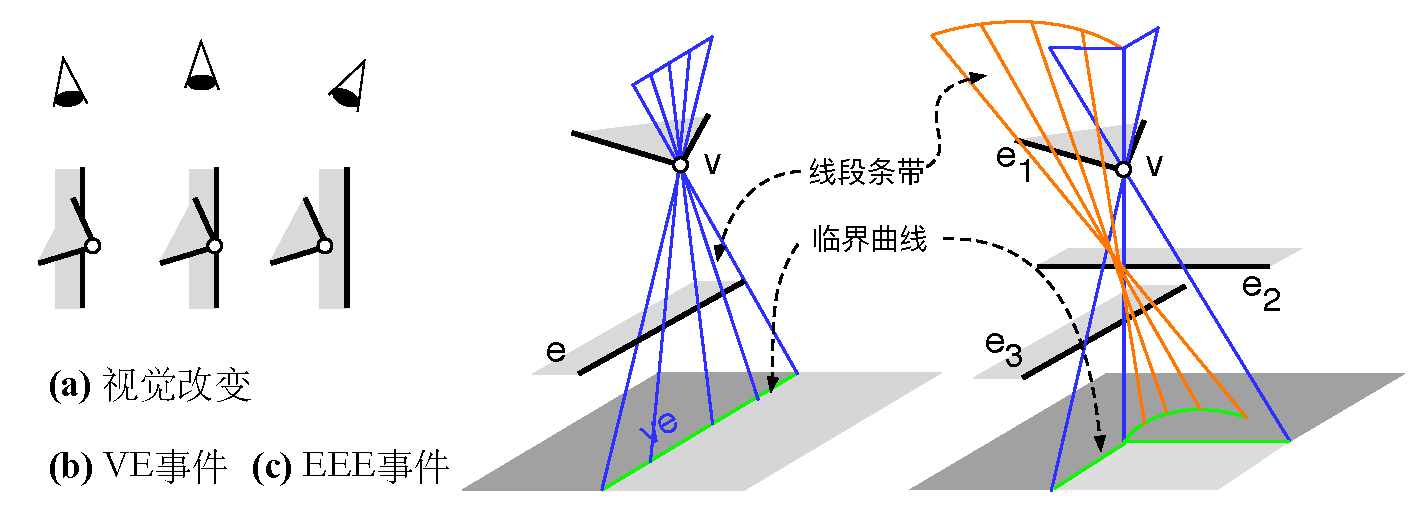
\includegraphics[width=1.\textwidth]{figures/r/visual-events}
	\caption{(a)视觉事件是由于可见性的改变形成的,它由一些曲面组成,这些曲面可由一些线段描述,(b)VE事件由所有同时穿过一个顶点$v$和一条边界$e$的线段构成;(c)EEE事件由所有同时穿过三条边界$e_1,e_2,e_3$的线段构成}
	\label{f:r-visual-events}
\end{figure}

当某个物体的表面与表述视觉事件的曲面相交时,其相交的曲线就形成了该表面的一条非连续边界线,如图\ref{f:r-visual-events}中的绿色线段所示,这些非连续边界线又称为临界曲线(critical curves)\myindex{临界曲线}{critical curves}。通过目前的知识可知,临界曲线的主要可以分为三类:即一个物体的某个边与另一个物体的某个面重合产生的$D^{0}$非连续边界,VE事件产生的线段条带与物体表面相交形成的临界曲线,以及EEE事件产生的线段条带与物体表面相交形成的临界曲线。

有了上述关于非连续边界线的概念描述,非连续网格化算法的步骤大概可以分为三步:首先找出每个表面的临界曲线,然后根据这些临界曲线对表面进行网格细分,最后对每个细分曲面选择合适的基函数以计算辐射度。我们将在下一节讨论第一步中涉及的非连续边界提取的问题,它涉及比较复杂的数据结构表述,然后在后面第\ref{sec:r-combine}节讨论后两个问题。




\subsubsection{提取非连续边界}\label{sec:r-critical-curves}
有了上述关于引起可见性改变的视觉事件的描述及分类,可见性边界的提取就变得比较简单了,例如我们只需要遍历场景中每个顶点-边界对(VE事件),以及所有的顶点-顶点-顶点(EEE事件)三元组以求出所有线段条带,让后再让这些线段条带与物体的所有面进行相交计算,这些线段条带与面的交线就构成了可见性边界。根据这样的思路,\cite{a:ADiscontinuityMeshingAlgorithmforAccurateRadiosity,a:DiscontinuityMeshingforRadiosity}能够处理VE事件形成的可见性边界,而\cite{a:Fastcomputationofshadowboundariesusingspatialcoherenceandbackprojections,a:AFastShadowAlgorithmforAreaLightSourcesUsingBackprojection}使用更一般的反向投影法(backprojection)\myindex{反向投影法}{backprojection}能够同时处理VE和EEE事件。

然而上述方法都有一个比较大的限制,那就是它们只能每次处理单个光源的视觉事件。回想视觉事件是指从某个点观察其可见性拓扑结构发生的变化,这个观察点实际上就是落于光源上的,因为通过这些观察点观察到的可见性事件才会形成阴影边界。所以对于每个视觉事件都对应着某个光源,如果有多个光源,上述这些算法要分别对每个光源执行一次可见性提取,我们称这样的算法为局部可见性算法。局部可见性算法对于多光源的计算成本非常高,并且它无法处理间接光照的阴影。

我们这里要介绍的是基于全局可见性(global visibility)\myindex{全局可见性}{global Visibility}的算法,在全局可见性算法中,它同时计算出所有顶点和边界之间的视觉事件(这和其他可见性算法的思路类似),并且使用一个巧妙的数据结构保存着所有可能的视觉事件之间的联系,使得我们可以快速查询对于任何观察位置的视觉事件,从而能够高效处理多光源的场景。这种特殊的数据结构称为可见性骨骼(visibility skeleton)\myindex{可见性骨骼}{visibility skeleton}\cite{a:TheVisibilitySkeleton:APowerfulAndEfficientMulti-PurposeGlobalVisibilityTool},它是可见性复合体(visibility complex)\myindex{可见性复合体}{visibility complex}技术\cite{a:The3Dvisibilitycomplex:anewapproachtotheproblemsofaccuratevisibility}的一个简化版本,以下我们就介绍可见性骨骼的数据结构以及构造方法,然后在第\ref{sec:r-combine}节将利用这些数据结构来实现网格细分。




\paragraph{可见性骨骼}
如上所述,线段条带是一些线段组成的曲面,线段条带中的线段具有一定的自由度,例如EV条带中的线段可以在边界$e$上自由移动,EEE条带中的线段也可以分别在三个边界$e_1,e_2,e_3$上自由移动,当这两种线段处于自由移动的极值位置时(即丧失移动的自由度),此时该线段称为极值线段(extremal stabbing line)\myindex{极值线段}{extremal stabbing line},极值线段是那些同时穿过4条边界的线段,例如以下是一些极值线段:

\begin{itemize}
	\item \textbf{VV线段}:VE条带中处于边界$e$的某个端点位置处的线段即为VV线段,此时两个顶点分别为两个边界的交点,所以该线段与四个边界相交。
	\item \textbf{VEE线段}:EEE条带中穿过其中的一个边界处于端点位置处的线段,此时该端点由两个边界相交组成,因此一共包含四条边界,如图\ref{f:r-visibility-skeleton}中的红色线段所示。
	\item \textbf{E4线段}:当EEE条带中的线段同时穿过第4条边界时,该线段一定为一个极值线段,可以参考\cite{a:TheVisibilitySkeleton:APowerfulAndEfficientMulti-PurposeGlobalVisibilityTool}中相关示例。
\end{itemize}

上述的线段条带与极值线段之间的相邻关系使我们可以定义一个由所有线段条带中的线段组成的线段空间(line-space)中一个图(graph),在该图中,每个节点是一条极值线段,而连接节点之间的连线则是与其相邻的线段条带。例如图\ref{f:r-visibility-skeleton}(b)中包含一个VEE极值线段($ve_1e_2$,红色线段),该极值线段即为一个节点,其相邻的两个线段条带$ve_1$和$ve_2$构成该节点的两个连线,如图\ref{f:r-visibility-skeleton}(a)所示。

\begin{figure}
\sidecaption
	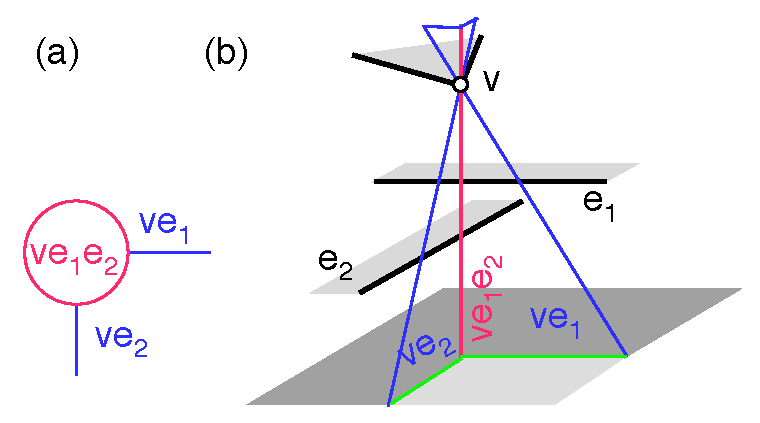
\includegraphics[width=.65\textwidth]{figures/r/visibility-skeleton}
	\caption{场景中的所有线段条带可以构成一个线段图,其中图中的节点为线段极值,每个节点的连线为该线段极值相邻的线性条带}
	\label{f:r-visibility-skeleton}
\end{figure}

我们的目标是要查询每个曲面所包含的线段条带,因为这些线段条带包含了该曲面的可见性信息。为了实现这个目标,原始的可见性骨骼技术\cite{a:TheVisibilitySkeleton:APowerfulAndEfficientMulti-PurposeGlobalVisibilityTool}使用了一个额外的数组来索引上述线段图中的节点,其数据结构如算法\ref{a:r-visiblity-skeleton}所示。

\begin{algorithm}
\begin{lstlisting}[language=C++, mathescape]
class Node {  // 线段极值,线段图中的节点
	List<Arcs> adjacentArcs 
	Face $F_{up}, F_{down}$ 
	Point3D $P_{up}, P_{down}$
}
	
class Arc {   // 线段条带,线段图中的连线
	Node $N_{start}, N_{end}$ 
	float $t_{start} , t_{end}$ 
	Face $F_{up}, F_{down}$
}
	
class EV : child of Arc {  // 所有EV条带,EEE条带省略了
	Edge e 
	Vertex v 
}
	
class VisibilitySkeleton { 
	tree<EV> ev$[F_{up} ][F_{down} ]$ 
	tree<EEE> eee$[F_{up} ][_{Fdown} ]$
}
\end{lstlisting}
\caption{描述曲面之间的可见性关系的一组数据结构称为可见性骨骼,其中Node和Arc类构成一个线段图中的节点和连线,而VisibilitySkeleton数组保存着曲面与线段极值节点的关系,该数据结构中的一些变量定义如图\ref{f:r-visibility-skeleton-structure-1}所示}
\label{a:r-visiblity-skeleton}
\end{algorithm}

对于初始的几何场景,首先对所有物体的每个顶点及边界进行遍历以计算出所有的极值线段(即Node对象),并使用光线投射计算出该极值线段对应的两个曲面索引$F_{up}$和$F_{down}$,以及其相邻的线段条带;接着这种对应关系被添加到VisibilitySkeleton数组中,并根据极值线段和线段条带的关系建立整个线段图;最后我们就可以通过两个曲面对$(P,Q)$通过VisibilitySkeleton数组查询P和Q之间的极值线段,从而可以得到相邻的线段条带,最终可以判断P和Q之间的可见性关系。

\begin{figure}
\sidecaption
	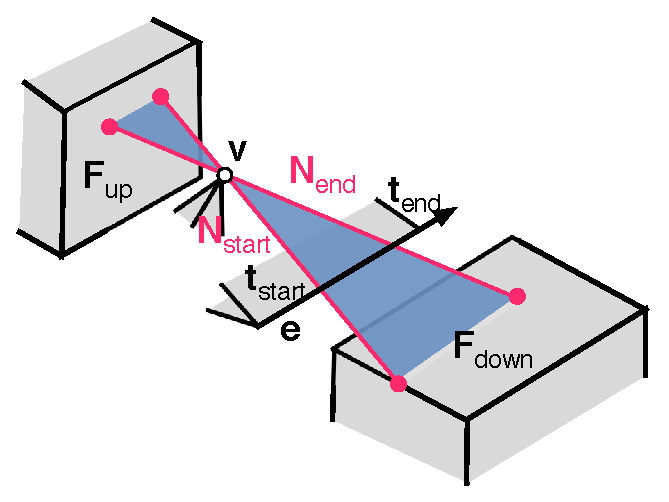
\includegraphics[width=.65\textwidth]{figures/r/visibility-skeleton-structure-1}
	\caption{描述线段条带的示意图}
	\label{f:r-visibility-skeleton-structure-1}
\end{figure}

上述的数据结构可以用于指导对曲面执行一次细分,然而却不适合我们下节将介绍的阶层式细分。为了实现阶层式细分,\cite{a:FastandAccurateHierarchicalRadiosityUsingGlobalVisibility}对上述的数据结构进行了修改,它直接将每个曲面的线段条带存储在该曲面自身的结构上,这样我们可以单独对该曲面进行细分处理。如图\ref{f:r-visibility-skeleton-structure}所示,每个曲面P自身存储着一颗二叉树,该二叉树的每个节点是所有与曲面P通过线段条带连接的曲面Q,由于每个曲面对P和Q之间可能存在多个线段条带,所以每个曲面对P和Q之间的所有线段条带被存储在另一个二叉树中,这样便可以通过曲面自己查询到所有可见的曲面及对应的线段条带。由此可以看出,每个线段条带将被引用两次,分别对应其相连的两个曲面。

\begin{figure}
\sidecaption
	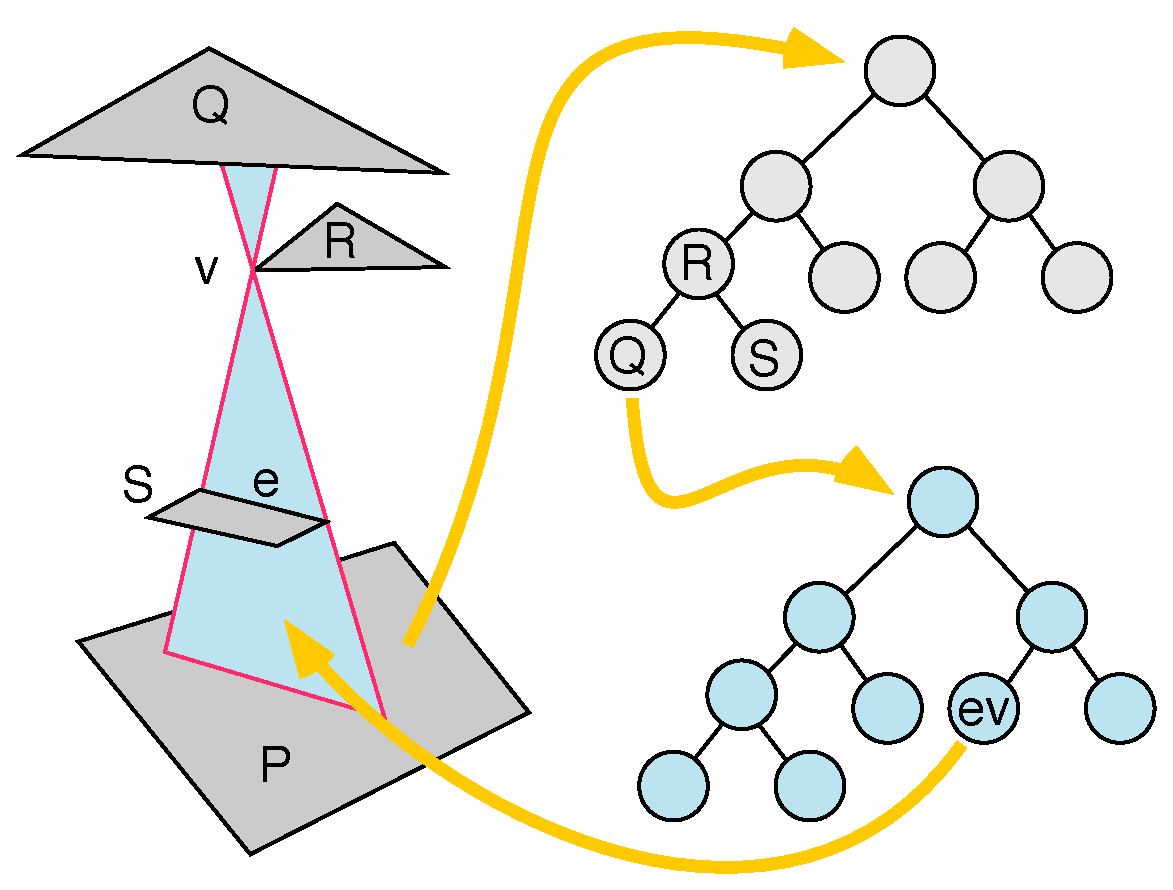
\includegraphics[width=.55\textwidth]{figures/r/visibility-skeleton-structure}
	\caption{为了便于阶层式细分,每个曲面包含的所有线段条带信息被存储在曲面自身的数据结构中,这通过两个二叉树来实现,首先右上角的二叉树存储着所有与该曲面相连的曲面,然而对于每个曲面对,右下角的二叉树存储着该曲面对之间所有的线段条带}
	\label{f:r-visibility-skeleton-structure}
\end{figure}

此外,以类似的方式,曲面的每个顶点v还存储着与该顶点通过线段条带连接的所有曲面Q,以及与这些曲面之间的线条条带,这反应的即是从V点观察到Q的可见部分,这被用于后面的阶层式细分,我们将在下节进一步讨论。

上述这两种针对每个曲面P的局部数据结构,其实正对应于传统的非连续网格化技术中针对单个光源存储的可见性信息,这里曲面P被视作为一个光源,它存储着所有与该光源相关具有可见性边界的曲面,同时也保存着该曲面每个顶点与这些交互曲面之间的线段条带信息。正是这种局部化的数据表述使得我们可以针对任意曲面计算其可见性信息,每个曲面都可以视作为一个光源,这正好可以处理二次以上的光线反射,在传统的非连续网格化技术中则做不到,因为它们只存储了每个光源几何体的可见性信息,因此不能处理间接光照的阴影分布。可见性骨骼这种对每个曲面可见信息的局部化表述形成一种全局的可见性数据。我们将在下一节进一步讨论这些数据的结构以及随着阶层细分过程的更新。





\subsection{组合方法}\label{sec:r-combine}
到目前为止,我们已经介绍了两种不同的曲面细分方法:即阶层式辐射度方法和非连续边界网格化,其中前者基于漫反射表面辐射度分布的低频特征,利用小波基函数的消失矩概念来减少形状系数的数量,因此计算效率比较高;而后者能够精确地辨识出物体表面由于物体间的遮挡关系产生的非连续边界,这些非连续边界被用于指导曲面细分,因而计算结果具有更高的精确性。这两种方法各自具有比较独立的优点,因此我们希望能将两种思路组合起来。

然而,这种组合在实践中却存在一些困难,其主要原因在于它们两种相互冲突的目标:阶层式辐射度方法希望使用非常简单的网格划分(例如层级之间基函数的单位尺度呈$2^{n}$关系),以实现高效的分解与合并操作;而非连续边界则要求使用尺寸和形状非常不规则的细分曲面,以更精确地表述辐射度分布的非连续性特征。

本节我们将介绍一种不同于传统阶层式辐射度方法的组合方法,这种方法能够适应不规则的细分曲面分布,同时尽管在很多方面它都具有不同的实现方式,但是最终却呈现出和阶层式辐射度方法类似的结构和特征,从而将两种不同的思路结合起来。




\subsubsection{形状系数的计算--顶点收集方式}
在开始介绍具体的算法之前,我们首先再深入讨论一下上述的两种局部数据结构,因为这种结构给出了一种新的计算形状系数的思路。这两种数据结构分别是关于每个表面与其他具有交互的表面之间的联系,以及每个顶点与其他具有交互的表面之间的联系,以下我们分别称之为面—面链接(polygon-polygon link)\myindex{面—面链接}{polygon-polygon link}和点—面链接(point-polygon link)\myindex{点—面链接}{point-polygon link}。

首先来看一下点—面链接,它决定了一种新的计算形状系数的方式。

前面介绍的形状系数都是通过称为曲面收集(patch gatering)\myindex{曲面收集}{patch gatering}的方式计算而出的,如图\ref{f:r-point-gathering}(a)所示,我们可以通过从接受面上的随机位置和随机方向向半空间发射光线,然后通过统计落于某个特定曲面的光线数量来计算两个曲面之间的形状系数,这形成一种按曲面为单位进行着色的效果。该形状系数可以看做是曲面中心点处的形状系数,如图\ref{f:r-point-gathering}(a)中的橙色圆点所示,为了计算每个位置处的实际形状系数,我们往往首先通过相邻曲面的形状系数推导出曲面顶点处的形状系数,如图\ref{f:r-point-gathering}(a)中的橙色箭头,然后再对曲面顶点处的形状系数执行双线性插值计算出每个给定位置(如图\ref{f:r-point-gathering}(a)中的红色圆点色)处的形状系数值,如图\ref{f:r-point-gathering}(a)中的红色箭头。

\begin{figure}
	\sidecaption
	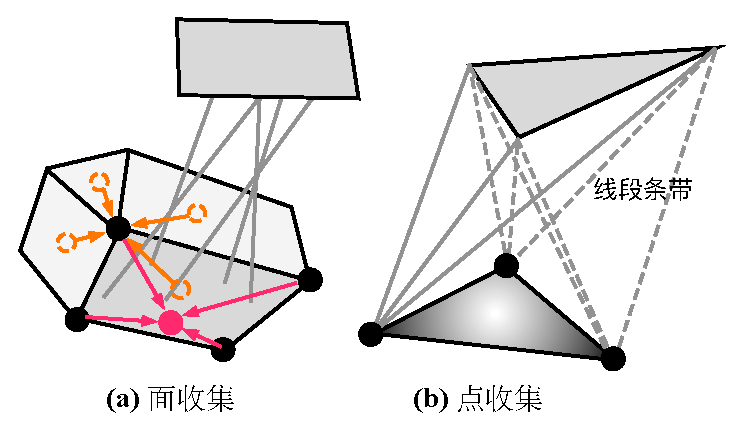
\includegraphics[width=0.65\textwidth]{figures/r/point-gathering}
	\caption{两种计算形状系数的方式:(a)面收集方法首先通过传统的方式计算曲面的形状系数,然后再推导出曲面顶点处的形状系数,最后对这些顶点执行线性插值计算每个给定位置处的形状系数;而(b)点收集的方法则直接计算每个顶点的形状系数,然后对其进行线性插值以计算每个特定位置处的形状系数值}
	\label{f:r-point-gathering}
\end{figure}

在上述的过程中,显然由相邻曲面推导出公共顶点位置处的形状系数的计算过程会产生一些误差。在可见性骨骼中,由于直接包含了每个顶点到相关曲面之间的线段条带,这可以直接用于计算基于点的形状系数,这种方法称之为点收集(point gathering),如图\ref{f:r-point-gathering}(b)所示,可以看出点收集能够直接产生更精确的顶点形状系数(因为它没有了近似推导过程),因此计算过程更叫高效和简洁。基于点收集的方法最早出现于\cite{a:Araytracingalgorithmforprogressiveradiosity}。

点—面链接的数据结构如算法\ref{a:r-point-polygon-link}所示。

\begin{algorithm}
\begin{lstlisting}[language=C++, mathescape]
class LinkPtPoly {
	List<Arcs> Arcs;  //每个边的线段条带
	Polygon Src;      //与之交互的曲面指针
	float FF          //形状系数
}
\end{lstlisting}
\caption{点—面链接数据结构,每个顶点自身存储了所有与该顶点交互的曲面,以及与该曲面之间的所有线段条带,这可以用于计算曲面对于该顶点的形状系数}
\label{a:r-point-polygon-link}
\end{algorithm}

有了点—面链接的数据结构,每个面Q到顶点v的形状系数可以通过下述的方式近似计算而出:

\begin{equation}
	F_{v,Q}= \cfrac{1}{2\pi}\vec{N}\cdot\sum\gamma_i \cfrac{\vec{R}_i\times\vec{R}_{i+1}}{||\vec{R}_i\times\vec{R}_{i+1}||}
\end{equation}

\noindent 这里的和是针对所有线段条带的,$\vec{R}$表示每个线段条带的极值线段,$\gamma_i$表示极值线段之间的夹角,如图\ref{f:r-point-polygon-link}所示。

\begin{figure}
	\sidecaption
	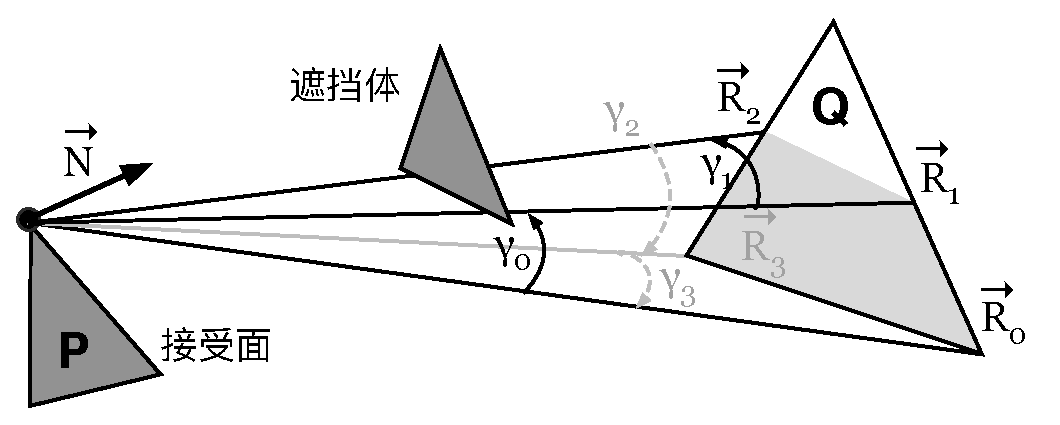
\includegraphics[width=0.62\textwidth]{figures/r/point-polygon-link}
	\caption{点—面链接数据存储了关于每个顶点与每个相关曲面之间的线段条带信息,这些信息可以直接用于计算该曲面对该顶点的形状系数}
	\label{f:r-point-polygon-link}
\end{figure}

此外,使用点收集的另一个好处是可以使用线性近似作为基函数来表述表面的辐射度分布,这比传统的阶层式辐射度方法使用常数函数的进行要精确一些,我们将在后面曲面三角化细分的时候讨论这种线性近似。

可见性骨骼也提供关于面与面之间的关系,即面—面链接,面—面链接的数据结构如算法\ref{a:r-polygon-polygon-link}所示,它存储的数据主要是曲面每个顶点对应的点—面链接数据。

\begin{algorithm}
\begin{lstlisting}[language=C++, mathescape]
class LinkPolyPoly {
	List<LinkPtPoly> ptPolyLinks;
	Polygon Src;
}
\end{lstlisting}
\caption{面—面链接数据结构,每个面存储了该面的每个顶点关于另一个曲面Src的点—面链接数据(如算法\ref{a:r-point-polygon-link}所示),面—面链接数据主要用于对曲面的细分计算,而不是传统的形状系数的计算}
\label{a:r-polygon-polygon-link}
\end{algorithm}

面—面链接数据结构其实可从图\ref{f:r-point-gathering}(b)中看出。理论上有些这样的数据我们可以计算出基于面收集的形状系数,但是面—面链接的数据却不是用于此目的,而是主要用于帮助指导后面会介绍的细分过程。




\subsubsection{三角化分解}
前面我们已经分过基于可见性边界信息的阶层式辐射度方法的困难,在传统的阶层式辐射度方法中,曲面的细分是基于所选择的小波函数,例如传统的哈尔小波基函数在不同分辨率之间使用$2^{n}$倍的尺度关系来对曲面进行阶层式细分,因此所得到的是一个高度均匀的细分结果。

然而非连续的可见性边界则天生是非均匀分布的,并且它从某种程度上已经“决定了”细分结果,所以我们不可能使用某种小波函数使得其细分的结果服从这种非均匀的分布,这是结合非连续网格化和阶层式辐射度方法的困难所在。

要克服这个困难,我们需要引入被称之为惰性小波变换的概念,




\paragraph{惰性小波变换}
对于一个连续的信号,我们可以在其定义域上的任意位置对其取样,因此通过任意小波函数由高分辨率向低分辨率进行分解得到的任意采样位置都能得到一个有效值,从而可以用这些位置的样本值来近似原始目标函数;然而对于有一些点集构成的离散信号,我们更希望直接使用这些离散值作为近似函数的样本值,因此人们提出一种称为提升方法lifting scheme)\mathindex{提升方法}{lifting scheme}的小波变换方法,该方法又称为前向小波变换(forward wavelet transform)\mathindex{前向小波变换}{forward wavelet transform},或者惰性小波变换(lazy wavelet transform)\mathindex{惰性小波变换}{lazy wavelet transform}。

不难看出,上述离散信号的条件和我们这里讨论的非连续边界的情况有些类似,即它们都是给出了一定的分解要求(如取样位置),使小波分解的结果满足这些要求。

让我们再对小波变换做一点深入分析,小波变换是一种将目标函数表述为(通过正交投影)一组满足小波函数特性的基函数的线性组合,它没有限定投影到每个基函数的方法(例如传统的哈尔小波变换由高分辨率向低分辨率的分解方法),也没有限定取样位置的分布(例如哈尔小波产生的均为位置取样),因此我们可以使用任意方法来产生到各个满足小波特性的基函数的正交投影。

哈尔小波给出了一种构造满足小波特性基函数的方法:低一级分辨率的尺度函数可以表述为高一级分辨率相邻两个尺度函数的和,而低一级分辨率的小波函数可以表述为高一级分辨率相邻两个尺度函数的差,如式\ref{e:r-harr-decompose}所示;根据这样的关系,我们同样可以得出由低一级分辨率的尺度和小波函数表述的高一级分辨率的基函数,如式\ref{e:r-harr-reconstruction}所示,这即是小波分析中的重建过程。

然而在重建过程中,我们假设小波函数的是未知的,对于任意一个新插入的位置(其产生更高的分辨率),例如那些已知的采样位置,我们可以通过该点的真实值计算出该位置处的小波函数系数。

\begin{figure}
\begin{fullwidth}
	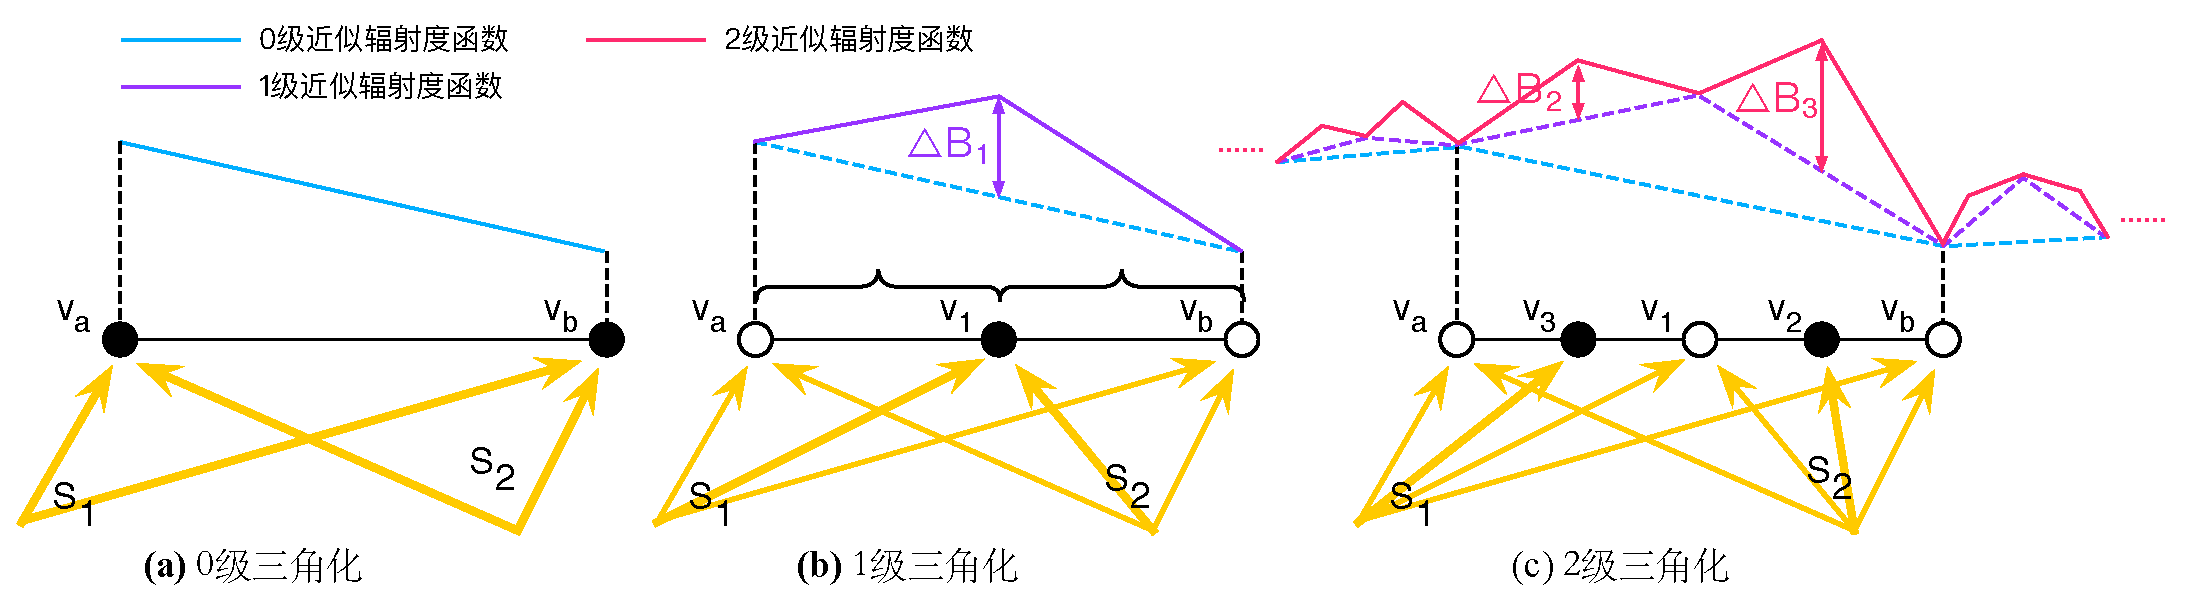
\includegraphics[width=\thewidth]{figures/r/triangulation}
	\caption{惰性小波变换采样了一种与传统小波变换相反的正交投影过程,它能够将一个目标函数投影到满足特定位置要求的小波基函数中}
	\label{f:r-triangulation}
\end{fullwidth}
\end{figure}

图\ref{f:r-triangulation}展示了这样的一个投影过程,从左到右我们将一个三角形执行后面即将介绍的三角化将其细分为更多三角形(当然这里为了方便仅图示了一个二维示意图),因此它也反映了由低分辨率向高分辨率的“重建”过程。对于每次插入的一个新的顶点,如图\ref{f:r-triangulation}(b)中的黑点,如果我们记录该点的值为该点的真实值与低一级分辨率辐射度函数近似的采样值的差$\Delta B$,即:

\begin{equation}
	\Delta B=B_l-\sum_{i=0..2}c_iB^{i}_{nl}
\end{equation}

\noindent 则这样的“重建”方式产生的小波函数将构成满足小波特性的基函数。这里$B_l$的值为位置$l$处的真实采样值,右边第二项则为该位置使用低一级分辨率近似的平均值,它由对三角形的三个顶点插值计算而来,其中$c_i$为相关的插值系数。直观上理解,在小波分解中,小波函数$\psi$的系数表述的正是高一级分辨率的尺度函数和低一级分辨率的尺度函数的差值。图\ref{f:r-triangulation}(c)展示了怎样通过上述过程的迭代产生高分辨率的函数近似,从而将目标函数投影到一组小波基函数中。

上述的过程和传统的小波变换的思路相反,传统的小波变换由高分辨率向地分辨分解,而惰性小波函数由低分辨率向高分辨率“重建”,所以这是称为前向小波变换的原因。“惰性”的称谓是因为直到给定了新的插值点才能确定其使用的小波函数$\psi$。




\paragraph{三角化}
以上我们给出了构造满足任意前置位置条件的小波变换的方法,剩下的问题就是如何对曲面进行细分,以满足(从可见性骨骼数据中)已知的可见性边界分布。

\cite{a:FastandAccurateHierarchicalRadiosityUsingGlobalVisibility}使用三角化的方式来构建阶层结构。通过迭代地对低分辨率的三角形执行约束德劳内三角化(constrained Delaunay triangulation, CDT)\mathindex{约束德劳内三角化}{constrained Delaunay triangulation}\cite{a:Hierarchicaltriangulationformultiresolutionsurfacedescriptiongeometricdesign},CDT允许对一系列表述多边形的点集执行包含某些预置线段的德劳内三角化\footnote{德劳内三角化是一种能够保证三角形的最小角最大化的三角化方法,因为最小角最大化能使三角化的误差更小。关于三角化相关内容请参阅计算几何相关的书籍,例如\cite{b:ComputiationalGeometry:AlgorithmsandApplications},本书的主要内容是聚焦于渲染,所以这里不会详述},在这里这些预置线段即是那些可见性边界线。

图\ref{f:r-hierarchical-triangulation}演示了使用CDT对几何场景执行三角化的过程,可以看到CDT三角化能够很好地适应场景的可见性分布,再加上前面惰性小波变换方法,这就是形成了称为可见性驱动的阶层式辐射度方法。

\begin{figure}
\begin{fullwidth}
	\begin{subfigure}[b]{0.245\thewidth}
		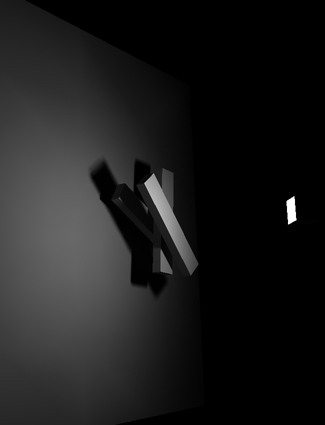
\includegraphics[width=1.\textwidth]{figures/r/hierarchical-triangulation-1}
		\caption{输入几何场景}
	\end{subfigure}
	\begin{subfigure}[b]{0.245\thewidth}
		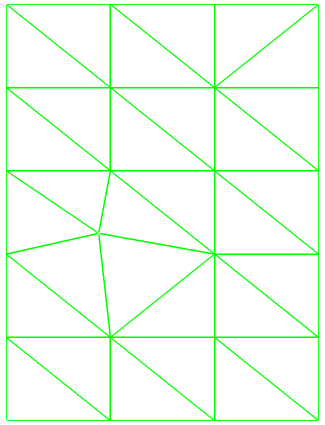
\includegraphics[width=1.\textwidth]{figures/r/hierarchical-triangulation-2}
		\caption{一级细分}
	\end{subfigure}
	\begin{subfigure}[b]{0.245\thewidth}
		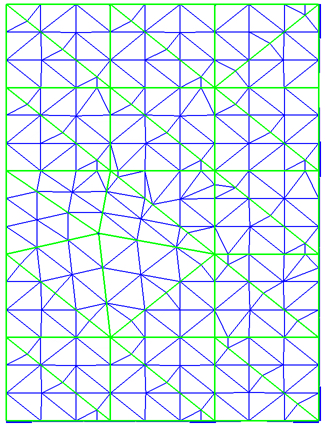
\includegraphics[width=1.\textwidth]{figures/r/hierarchical-triangulation-3}
		\caption{二级细分}
	\end{subfigure}
	\begin{subfigure}[b]{0.245\thewidth}
		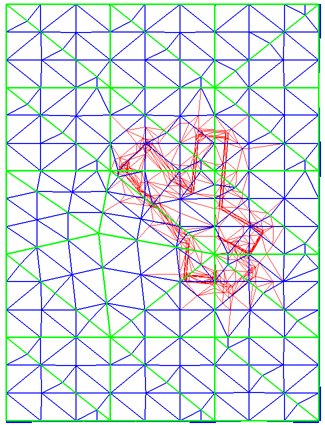
\includegraphics[width=1.\textwidth]{figures/r/hierarchical-triangulation-4}
		\caption{三级细分}
	\end{subfigure}
	\caption{阶层式三角化细分,这样的细分能够适应可见性边界的分布。场景中右边为一个面积光源(图片来自\cite{a:FastandAccurateHierarchicalRadiosityUsingGlobalVisibility})}
	\label{f:r-hierarchical-triangulation}
\end{fullwidth}
\end{figure}




\subsubsection{可见性更新}
经典辐射度方法使用一个常数尺寸对场景进行一次细分,因此每个细分曲面的尺寸都一样,这样虽然操作简单,然而却存在一些弱点:例如对于那些没有被遮挡的表面,这样的细分往往太过精细而浪费了内存和计算资源,而对于那些可见性比较复杂的区域,这样的细分可能又由于不能区分这些可见性边界而导致较大的误差。非规则细分的辐射度方法就是要消除这两个问题,它们使用一个称谓细化(refinement)\myindex{细化}{refinement}的过程来使细分达到足够的精度,这个精度要求可能是一个误差阈值,它被用于指导何时需要进一步对曲面进行细分。例如在阶层式辐射度方法中,如算法\ref{a:r-hierarchical-radiosity}所示,那里使用一个最小形状系数值$F_{eps}$来指导对曲面的进一步细分;传统的小波辐射度方法则相反,它们首先使用采样定理将采样分辨率提高到一个足够的精细度,然后逐级分解剔除那些较平坦区域的系数\footnote{这从某种程度上看有点类似于“反细化”(或者平滑)的过程。}。

不管怎样,细化策略给了一个标准要求,使我们必须保留目标函数的一些足够的细节。本节我们将介绍如何对上述三角化阶层式辐射度方法进行细化以及使用什么样的标准来指导细化。

\begin{myshaded}
	注意这里的细化和前面介绍的三角化分解的区别:
	
	在传统的阶层式辐射度方法中,这两个概念其实是一个过程,即直接对曲面进行细分,例如一个曲面没细分为四个相同尺寸的四边形子曲面;然而在基于可见性驱动的阶层式辐射度方法中,由于可见性边界的分布极其不规则,因此由可见性边界导致的细分曲面结构往往非常复杂,例如可能包含不等边数的多边形结构,这给计算带来一定的复杂度,所以为了简化这种复杂度,我们还需要对细分后的不规则多边形结果执行一个三角形的过程将其转变为规则的三角多边形分布,尽管这些三角形的几何分布仍然及其不规则,但是对于三角化网格已经有许多成熟的处理算法。
	
	所以,这里讨论的细化过程其实才是真正的基于可见性边界的曲面细分,三角化也会产生新的子曲面,但是如果没有细分的需要,则也就不会包含后续三角化的需要。
\end{myshaded}

以下首先介绍对曲面根据可见性边界进行细化的方法,然后讨论相应这些细化方法的标准。




\paragraph{链接细化}
由于曲面的几何信息表述为链接数据,如点—面链接和面—面链接,所以细化的过程实际上是链接数据的细化过程。

链接细化(link refinement)\myindex{链接细化}{link refinement}其实也很简单,有后面的内容可知,细化的结果其实就是对当前几何多边形插入一些点(如极值点)或者一些线段(如可见性边界),细化后的多边形必须包含这些点(作为顶点)或者线段(作为边),由于链接数据包含针对每个顶点的点—面链接数据,以及针对面的面—面链接数据,所以我们只需要对这些新的点和面构建对应的链接数据。

由于链接数据涉及两个曲面,即光照由一个表示光源的曲面传输到一个表示接受面的曲面,所以存在两类细化(其具体发生何种细化由后面的细化标准决定):

\begin{itemize}
	\item 光源细化:此时光源上各个点的辐射亮度分布的变化比较大。
	\item 接受面细化:此时对接受面的采样点过于稀疏,可能忽略一些细节,例如一些极值。
\end{itemize}

光源细化是指几何细分仅发生在光源上,即光源被细分为多个子(三角)曲面(例如由于物体遮挡导致光源的分布发生了显著变化,如图\ref{f:r-source-refinement}(c)所示),所以对于每个接受该光源曲面光照的接受面,它的每个顶点的点—面链接数据需要更新,此时每个顶点由原来连接的一个面变为多个面,单个顶点新增的线段条带如图\ref{f:r-source-refinement}(d)所示,图\ref{f:r-source-refinement}(b)为细分后P点的视图,红色箭头都是表示要修改或新增的线段条带。

\begin{figure}
\begin{fullwidth}
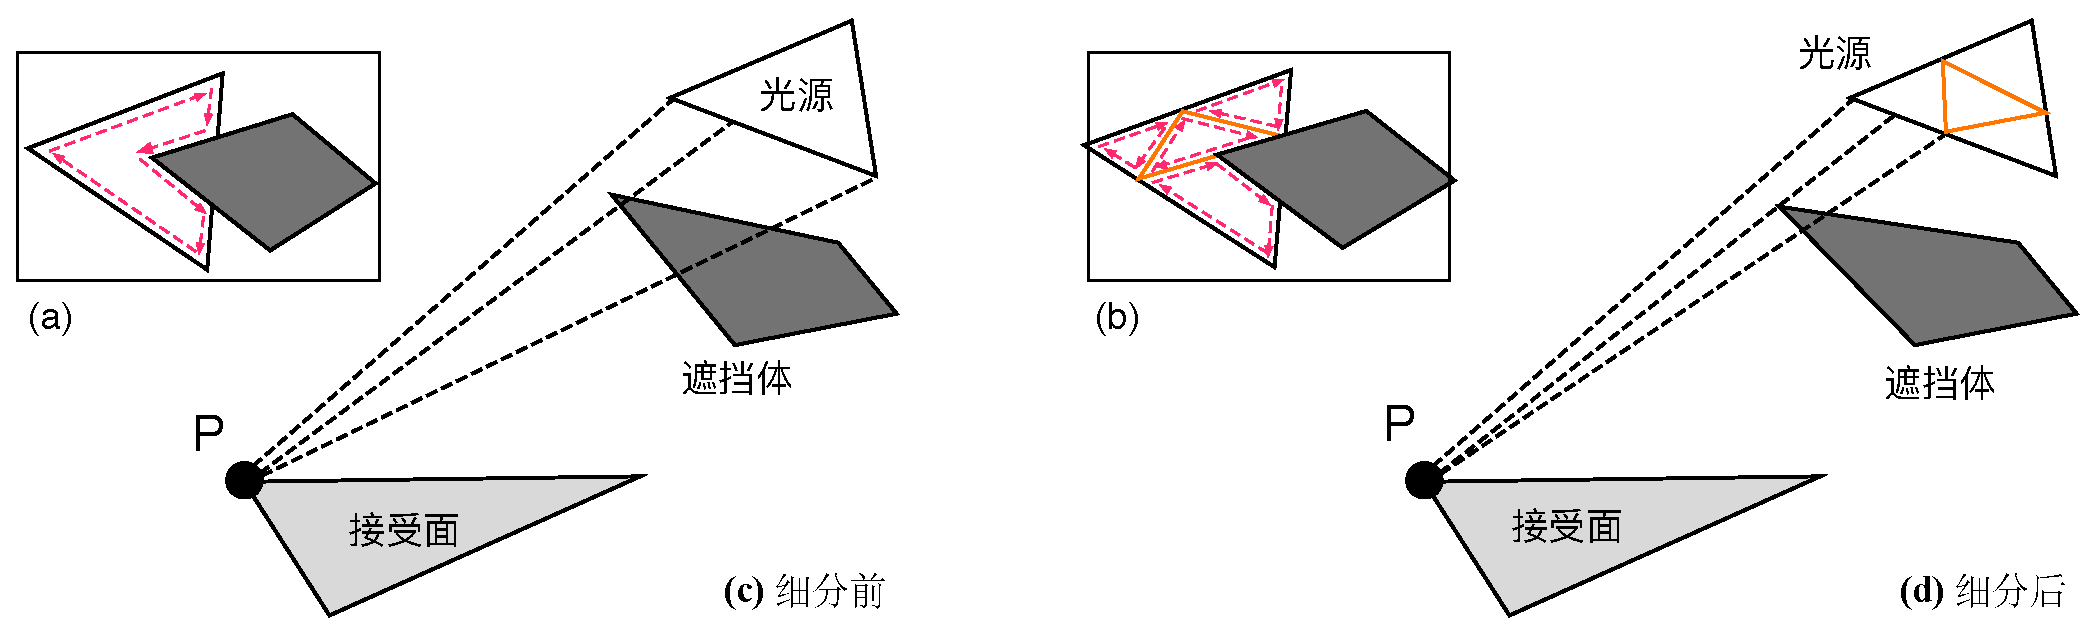
\includegraphics[width=\thewidth]{figures/r/source-refinement}
	\caption{当发生光源细化时,由于原来接受面链接的一个光源曲面变为多个光源子曲面,所以我们需要分别更新接受面每个顶点的点—面链接数据和该面的面—面链接数据。(a)和(b)中的红色箭头表述顶点P的在细分前后的线段条带}
	\label{f:r-source-refinement}
\end{fullwidth}
\end{figure}

此外,每个接受面的面—面数据也需要更新,因为原来的单个面—面链接变为与多个光源子曲面的面—面链接。

需要注意的是,所以的可见性更新都发生在2D空间,即变量光源的每个曲面的每个子边,然后检测改变与顶点P组成的平面是否与场景中的其他物体相交;由于每个面记录了与其所有线段条带相交的遮挡体列表,所以执行可见性更新时只需要遍历这些遮挡体即可。

另外,值得说明的是,虽然对于光源的细分,从光源的每个细分曲面来观察,它的视图结构也发生了变化,但是我们并不对这些顶点存储新的(点—面和面—面)链接数据,因为这里我们是需要计算该(细化前的)光源曲面对接受面的光照贡献,即这里要计算接受面的形状系数。实际上,光源的这种几何细化仅是针对当前这个接受面才有意义,因为这种细分是由它们之间的遮挡关系决定的。因此,所谓的全局可见性信息并不是说每个可见性边界都是全局可见的,那样将没有意义,并且增加每个顶点计算的遍历成本。相反,可见性骨骼是由一个树形网格结构来保存每个曲面和顶点对应的可见性信息,这样保证了每个顶点只需要处理从该顶点观察的可见性数据,并且可以对每个曲面进行独立的几何细分,每个曲面的细分并不受其他曲面可见性信息的影响。

\begin{figure}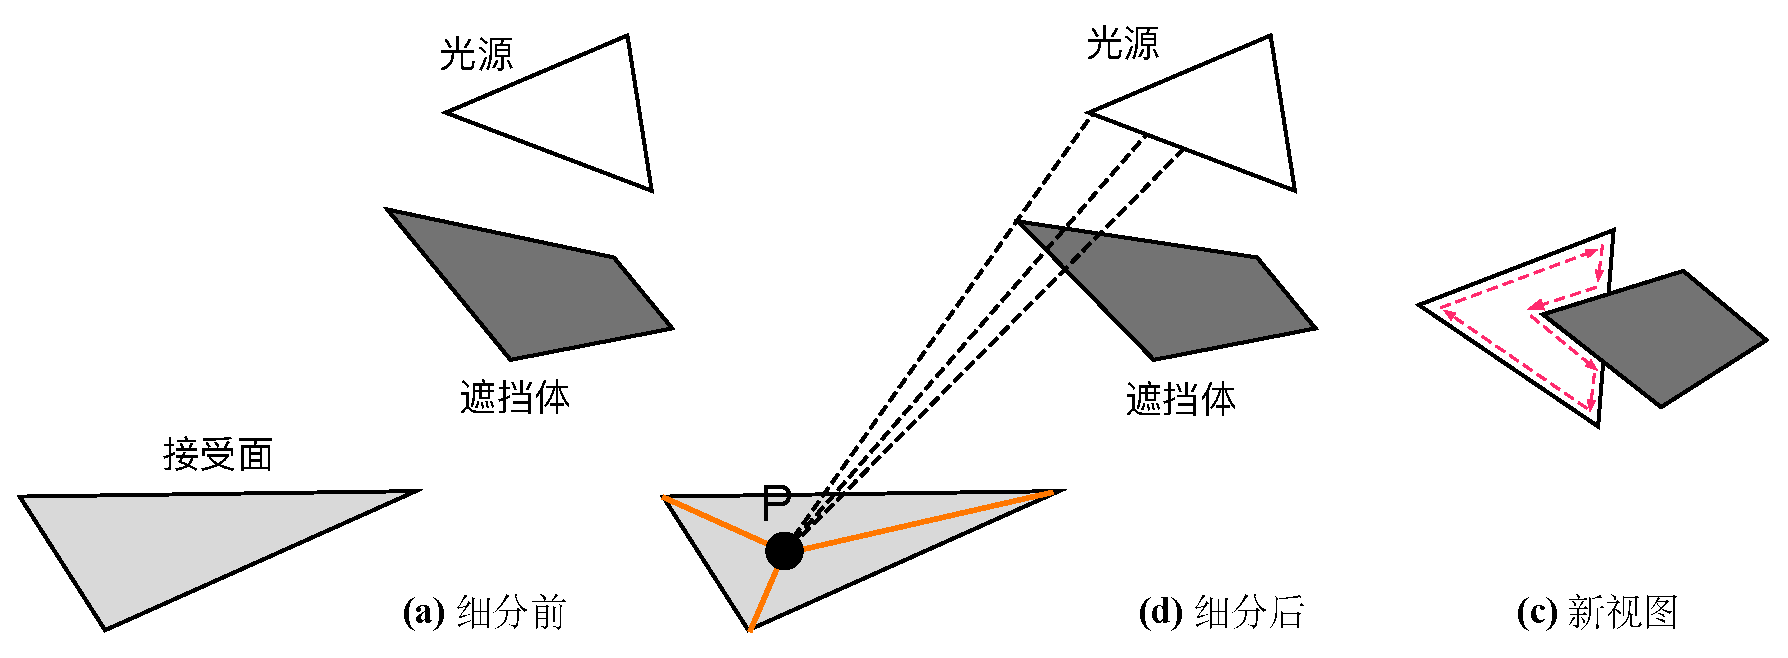
\includegraphics[width=1.\textwidth]{figures/r/receiver-refinement}
	\caption{当发生接受面细化时,新的顶点被条件到接受面形成新的细分曲面,由于我们需要计算新插入的顶点P的形状系数,因此新的链接数据被添加。对于(b)这种单个顶点的情况,实际上只需要计算P点的可见性数据即可(c),同样,它仅需要对当前接受面的遮挡体列表进行测试}
	\label{f:r-receiver-refinement}
\end{figure}

对于接受面细化,情形稍微复杂一点,因为它创建了新的曲面和顶点,如图\ref{f:r-receiver-refinement}(b)所示,所以我们要在可见性骨骼上添加新的曲面和顶点,因为这些顶点需要计算形状系数。新的顶点P的的试图节线段条带如图\ref{f:r-receiver-refinement}(c)所示。



\paragraph{细化标准}
以上我们介绍了曲面细化的方法,那什么时候或者说在什么条件下需要对曲面执行进一步细化呢?

当然这里也可以使用阶层式辐射度中使用的最小形状系数阈值作为细分依据,\cite{a:FastandAccurateHierarchicalRadiosityUsingGlobalVisibility}使用了一种基于视觉的(perceptually-based)\myindex{基于视觉的}{perceptually-based}细分标准。

人眼对颜色变化的感知更强于对颜色本书的辨识,例如我们通常靠物体的形状边界来记忆和识别物体,心理视觉研究\cite{a:Perceptually-drivenradiosity,a:Colordisplaysandcolorscience}表面,人眼可辨识2\%的差异,这又称为最小可觉差(just noticeable difference)\myindex{最小可觉差}{just noticeable difference},以下我们将用一个误差$\varepsilon_{percep}=2\%$来作为后面所有细分的标准。

\cite{a:FastandAccurateHierarchicalRadiosityUsingGlobalVisibility}提供了多种细化的选择或者说步骤。首先,他们发现在头两个级别使用可见性边界作为细分依据会导致一定的视觉痕迹,所以头两个级别通过以几何尺寸为依据使用比较均匀的网格划分,如图\ref{f:r-hierarchical-triangulation}(b)和(c)所示。

其次,在执行第一次细分前,还需要执行一个最大值搜索。\cite{a:Accurateandconsistentreconstructionofilluminationfunctionsusingstructuredsampling}指出提取出场景中具有最大光照值的极值点将能够增加辐射度计算的精确度,但是对于太小面积的曲面执行极值提取意义不大,所以仅在第一次细分前对最大分辨率的场景执行一次极值搜索,可以通过使用梯度信息找出极值点,后面的细化过程需要计算这些极值点的链接数据。此外,这些极值点和上面介绍的头两个级别的均匀细分会混在一起,导致细分不规则,所以在这里两个阶段比较靠近极值点的顶点会被舍弃,这使\ref{f:r-hierarchical-triangulation}(b)和(c)中出现一定的“弯曲”,这些即是极值点。

第三,是基于辐射度分布的细化,这主要是检测(在不考虑遮挡的情况下)辐射度的线性分布表述是否足够精确,例如检测曲面中心位置,各个边中点位置与各个顶点辐射度差异是否大于$\varepsilon_{percep}$,是则需要对曲面进行进一步细化。

最后,是基于可见性信息的细化,这主要是检测遮挡阴影对于辐射度分布的影响。例如对于每个视觉事件(即某个顶点包含的某个线段条带),如果线段条带将光源分割的两个部分对顶点的辐射度的差异大于$\varepsilon_{percep}$,则我们应该对光源按照该线段条带执行光源细分,如图\ref{f:r-source-refinement};再比如对于接受面,如果整个接受面的面积大于面积光源导致半影的面积,则说明由完全不被遮挡的区域存在,此时应该对半影可见性边界执行细化,即对接受面很执行接受面细分,如图\ref{f:r-receiver-refinement}所示。当然,如果为遮挡区域与半影区域辐射度变化小于$\varepsilon_{percep}$,则不需要进一步细分。




\section{Enlighten中间件}\label{sec:r-enlighten}
Enlighten\footnote{\url{http://www.geomerics.com/enlighten/}}是时下非常流行的基于辐射度方法的全局光照解决方案,它以中间件的形式提供,可以很容易地集成到已有的渲染引擎中去,它甚至已经被集成为Unity内置的实时全局光照解决方案。

本节将对Enlighten做简要的介绍,当然这里不是要介绍Enlighten的接口及使用,而是结合前面介绍的辐射度方法理论对Enlighten的架构进行一些简要的分析,使我们能够对辐射度方法怎样被用于实时渲染有更清晰的思路,从而加深对辐射度方法的理解。不过由于Enlighten并无多少公开的资料,所以这里仅做比较有限的讨论。



\subsection{Enlighten概述}
光线路径的计算非常复杂,所以实时渲染通常无法完全处理所有完整的光线路径,并且严重依赖于一些近似模型或者预处理技术来实现全局光照。一般的实时渲染全局光照模型(至少)包含以下三部分(如图\ref{f:r-real-time-gi}所示):

\begin{itemize}
	\item 直接光照(direct lighting)\myindex{直接光照}{direct lighting}:即由摄像机发出光线经过一次场景交互(反射或折射)后直接到达光源的路径,其中光线与场景的可见性测试由光栅化的深度剔除决定,而光线与光源的可见性测试则由阴影贴图(shadow map)\myindex{阴影贴图}{shadow map}决定(阴影贴图是将摄像机置于光源处的光栅化渲染结果)
	\item 间接光照(indirect lighting)\myindex{间接光照}{indirect lighting}:即所有二次以上反弹的光照,在实时渲染领域这通常仅指由光源发出光线经过零次或多次场景交互最后落于漫反射表面的间接光照,因为落于漫反射表面的光照是与观察方向无关的,所以可以被预处理并缓存起来,这在实时渲染中一般指光照贴图(light map)\myindex{光照贴图}{light map}。
	\item 光泽反射(specular lighting)\myindex{光泽反射}{specular lighting}:即与观察方向有关的光泽反射光照,它们一般通过环境贴图(environment map)\myindex{环境贴图}{environment map}来实现(假设被照射的物体距离周围环境比较远,例如天空环境之于地面,因此来自环境的光照可以认为是与物体表面上的位置无关的,所以周围环境可以被一个2D的方向变量索引,这使得环境光照被存储到一个2D纹理中,从而能够实现光泽或镜面反射)。
\end{itemize}

上述三类光照分量及其技术几乎是现代实时渲染引擎最基本的要求,它们的各自的效果及组合可由图\ref{f:r-real-time-gi}所示,我们这里聚焦于使用Enlighten中间件解决间接光照部分,本书的后续章节还会介绍更多的实时全局光照技术。

\begin{figure}
	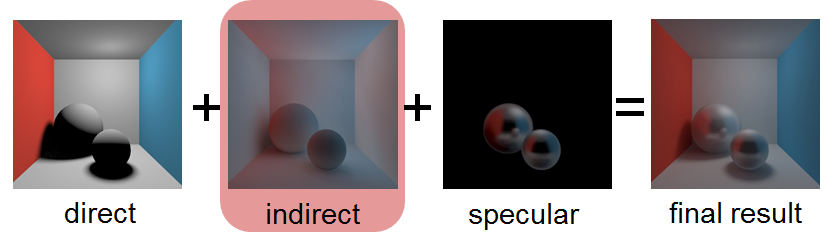
\includegraphics[width=1.0\textwidth]{figures/r/real-time-gi}
	\caption{现代实时渲染引擎需要实现最基本的光照分量,对于静态的场景,这些光照分量都可以被很好的预处理并使用贴图技术快速渲染,然后对于动态场景则要求更复杂的一些技术}
	\label{f:r-real-time-gi}
\end{figure}

Enlighten着重于解决间接光照部分,这也是最复杂的部分。虽然传统的光照贴图具有非常高的质量,但是它只能处理静态场景,一旦光照被烘焙到光照贴图中后,场景中的光源及材质等信息均不能被修改,否则需要重新烘焙光照贴图,这限制了光照贴图的使用。而辐射度方法仅预计算场景中的几何可见性关系,并且其辐射度线性方程组可以被快速求解,所以这允许程序在运行时对不涉及几何可见性的属性进行修改,例如材质的(漫)反射系数,表面是否发射光照的启用与关闭,光源光照的强度等,借助于后面介绍的从光栅化直接光照结果中进行点采样,Enlighten甚至允许光源的移动等任意修改。

为了方便地集成到各个渲染引擎中,Enlighten被设计为一个中间件,它对输入的静态场景几何数据进行处理,然后输出一些能被传统渲染引擎使用的数据,这包括:

\begin{itemize}
	\item 光照贴图(light map)\myindex{光照贴图}{light map}:和传统的光照贴图一样\footnote{实际上还是有差别,由于Enlighten使用的是辐射度方法,因此光线路径中不包含任何光泽或镜面反射的路径,而传统的光照贴图是可以包含光泽或镜面反射路径的,只要最终存储的位置位于漫反射表面上即可,这和光子映射技术中的光子的路径是类似的。},实际上也可以使用Enlighten来烘焙光照贴图,然后在运行时不使用Enlighten的运行时组件。
	\item 光照探针(light probe)\myindex{光照探针}{light probe}:无论是Enlighten还是传统的光照贴图均无法处理可移动的物体,然而对于间接漫反射光照,由于其频率变化较低,所以我们可以使用球谐函数缓存空间中一些位置的辐射照度,然后通过插值计算出动态物体表面的间接漫反射光照。
	\item 反射捕获(reflection capture)\myindex{反射捕获}{reflection capture}: Enlighten也可以输出来自漫反射表面的环境贴图,用于实现来自间接漫反射光的光泽反射效果。
\end{itemize}

本章仅聚焦于光照贴图,光照探针和反射捕捉相关的知识留在后续章节中介绍。

Enlighten的计算过程由一个预计算过程和运行时过程组成,这两个阶段均发生在CPU端,其中预处理过程发生于游戏设计开发阶段,它将输入的场景几何数据转换为一组可为运行时实时计算光照的数据,这其实主要就是场景表面之间的形状系数;然后在运行时阶段,Enlighten使用这些预处理的数据以及场景中的光照,材质等信息实时地求解辐射度线性方程组,并输入上述光照输出数据被渲染引擎使用。

以下就以Enlighten计算的过程为线索,对Enlighten的架构知识进行进一步讨论。




\subsection{预处理阶段}
Enlighten的预处理过程可以分为三个阶段,即对纹理坐标打包,将几何场景细分成簇,以及计算簇之间的形状系数,以下分别讨论。



\subsubsection{打包}\label{sec:r-packing}
预处理的第一个阶段称为打包(packing)\myindex{打包}{packing},它主要是生成后面光照贴图的纹理坐标UVs数据。

UVs表示一个纹理对应的纹理坐标数组,它们是一些2D的坐标值,其坐标轴为U和V,它们可以被映射为物体表面的3D位置。一般的UVs只存储三角形顶点处的坐标值,纹理坐标数组被光栅化插值之后得到贴图上各个像素的纹理坐标值,该坐标值被着色器用于获取光照贴图中的颜色值。每个(包括传统的和这里Enlighten生成的)光照贴图都需要一个UVs数组以对物体表面进行着色。

在UVs中,具有公共顶点的三角形组成一个图表(chart)\myindex{图表}{chart},在光照贴图中它代表一块连续的区域,这块区域也是来自于同一个物体的某一部分或全部表面。例如图\ref{f:r-packing}右下角的彩色方块就表示图中对应场景中各个表面对应的图表,图表视图对应的布局也即是最后光照贴图中各部分颜色的分布。每个图表中的线段图表示该图表对应的几何网格以及位置。

\begin{figure}
\begin{fullwidth}
	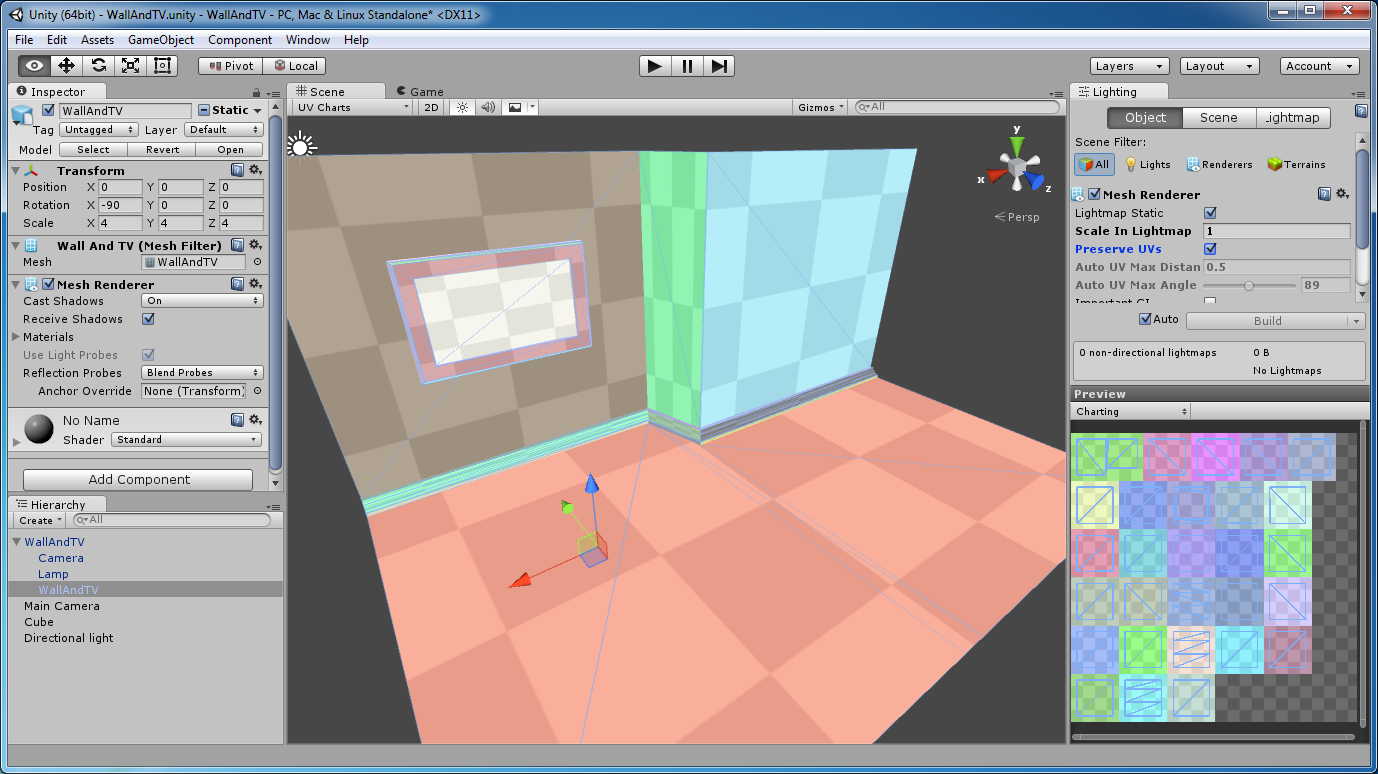
\includegraphics[width=1.0\thewidth]{figures/r/packing}
	\caption{在Enlighten的预处理阶段,首先将每个物体表面的纹理坐标打包成一些图表,多个相关的图表构成一个光照贴图(即对应一个系统),右下角的图表视图显式了场景中的各个物体表面怎样被打包,每个图表对应光照贴图部分的分辨率可以被修改以适配不同的光照分布,图表也可以被合并形成更稀疏的表格分布(图片来自\cite{a:ARMGuideforUnityDevelopersOptimizingMobileGamingGraphics})}
	\label{f:r-packing}
\end{fullwidth}
\end{figure}

在接下来的聚类阶段,Enlighten会将多个图表合并到一个系统(system)\myindex{系统}{system}上,每个系统即对应一个光照贴图,根据不同的系统划分,同一光照贴图上的图表可以来自多个不同物体的表面。

传统的光照贴图包含直接光照及阴影,所以要求比较高的分辨率以精细表述物体表面的颜色分布,然而Enlighten生成的光照贴图仅表示间接漫反射的光照,其频率变化非常小,并且光照贴图的分辨率影响着预处理及实时计算的效率,所以Enlighten中的实时光照贴图会使用比较小的分辨率。在Unity中默认使用每单位$4\times 4$个像素,也可以通过修改\textbf{Min Chart Size}参数为2,以设置最低分辨率为每单位$2\times 2$个像素。此外,还可以根据物体的光照分布单独调整单个物体的分辨率,这通过修改\textbf{Scale In Lightmap}参数实现。

我们可以直接使用几何网格自带的UVs数据,或者在导入的时候由Unity自动生成,如果是前者则需要打开\textbf{Preserve UVs}选项,如图\ref{f:r-packing}就是使用了网格自带的UVs数据。

图表的尺寸和数量与光照贴图中像素的数量存在着一定的联系,较大尺寸(因此数量更少)的图表往往只占据更少的像素,而具有更多细节(因此数量更多)的小图表则会占用更多的像素,其原因将在本节末单独讨论。\textbf{Preserve UVs}往往包含较复杂的细节,所以为了提高预处理及实时计算的效率,这需要对UVs进行一定的简化,当\textbf{Preserve UVs}选项被禁用时,Unity会默认生成一个简化的UVs,这也是默认的方式。简化的UVs会尝试合并一些具有较小细节的图表,例如图\ref{f:r-packing}中墙面与地面相交部分的墙角线的间接漫反射光照相较于整个室内环境完全可以忽略掉,图表合并的效果也可以由图\ref{f:r-chart-merging}所示。

\begin{figure}
	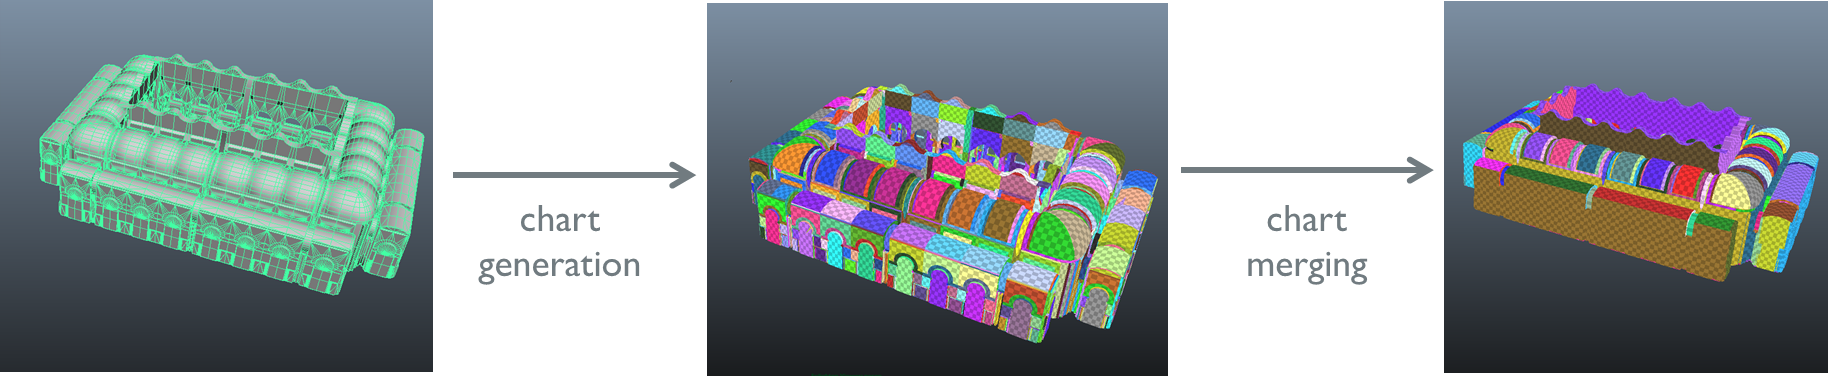
\includegraphics[width=1.\textwidth]{figures/r/chart-merging}
	\caption{图表合并能够平滑物体表面的多个细节,使得更大面积的表面可以被更少的纹素表示,因此大大提高了计算效率,图中距离较远一边的房屋顶面的多个图表被使用一个单一的图表(紫色所示)替代,该图表只需要很少的纹素即可表述}
	\label{f:r-chart-merging}
\end{figure}

有两个选项可以控制图表的合并以生成更简化的图表,\textbf{Auto UV Max Distance}告诉Enlighten对两个距离小于该值的图表进行合并,而\textbf{Auto UV Max Angle}则会合并两个夹角小于该值的图表,\textbf{Auto UV Max Angle}的默认值为89,以防止那些相互垂直的图表被合并。




\paragraph{为什么图表的尺寸和数量影响着光照贴图纹素的数量}
表面上看,光照贴图中纹素的数量仅与各个物体的分辨率设置(即\textbf{Scale In Lightmap}参数)有关,那为什么合并为简化的图表或者说减少图表的数量可以减少纹素的数量呢?

Enlighten中的光照贴图被设计为最小每单位$2\times 2$像素,并在运行时处理光照贴图时针对此进行了优化,所以每个图表至少占据$2\times 2$个纹素。这样的设置也是上述讨论的图表合并功能的需要,因为两个图表可能具有不同的分辨率设置,所以如果它们的图表紧挨在一起时,在被转换为真实分辨率的时候就会导致重合,所以Enlighten总是保证图表边缘预留半个像素的位置,这就也要求每个图表至少占据$2\times 2$个纹素。

由于限定了每个图表最少占据4个纹素,这就会导致一定的浪费,例如在图\ref{f:r-charts}中,梯子的边缘处包含一个棱角边,本来只需要一个像素,然而现在每个棱边都需要$2\times 2$个纹素,如果\textbf{Min Chart Size}被设置为4,则整个楼体占据$70\times 72$个纹素。

\begin{figure}
	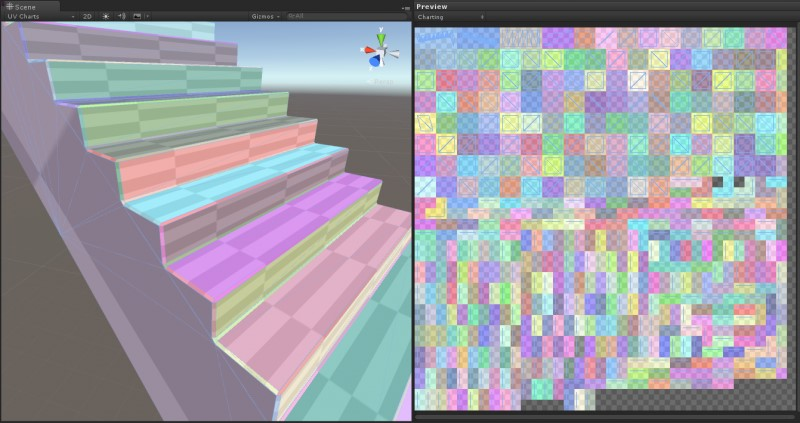
\includegraphics[width=1.\textwidth]{figures/r/chart}
	\caption{场景中的棱边,线段以及一些微小的细节可能占用大量不必要的纹素资源,这些细节相对于间接漫反射光照通常是可以忽略的,通过合并图表,光照贴图的分辨率可以进一步被降低(图表来自\cite{a:AwesomeRealtimeGIondesktopsandConsoles})}
	\label{f:r-charts}
\end{figure}

由于棱边的间接漫反射光照可以忽略不计,我们可以将棱边与梯面合并起来,而每个梯面只需要$2\times 2$个纹素即可表述,因此设置\textbf{Min Chart Size}为2,经过图表合并后的光照贴图可以仅占据$22\times 24$个纹素\footnote{在Unity中也能通过\textbf{Edge Stitching}参数自动处理这类物体边界线的视觉问题。}。




\paragraph{系~~统}
相对传统的辐射度方法,Enlighten针对实时渲染的一个主要优化是引入了称为系统(system)\myindex{系统}{system}的概念,系统是由Enlighten自动对场景中的物体进行划分产生的\footnote{在Unity中也能通过\textbf{System Tag}参数手动设定,该参数会强制创建新的系统和光照贴图。},一个系统是指多个物体(或者说图表)共享一个光照贴图。

\begin{figure}
	\begin{subfigure}[b]{0.285\textwidth}
		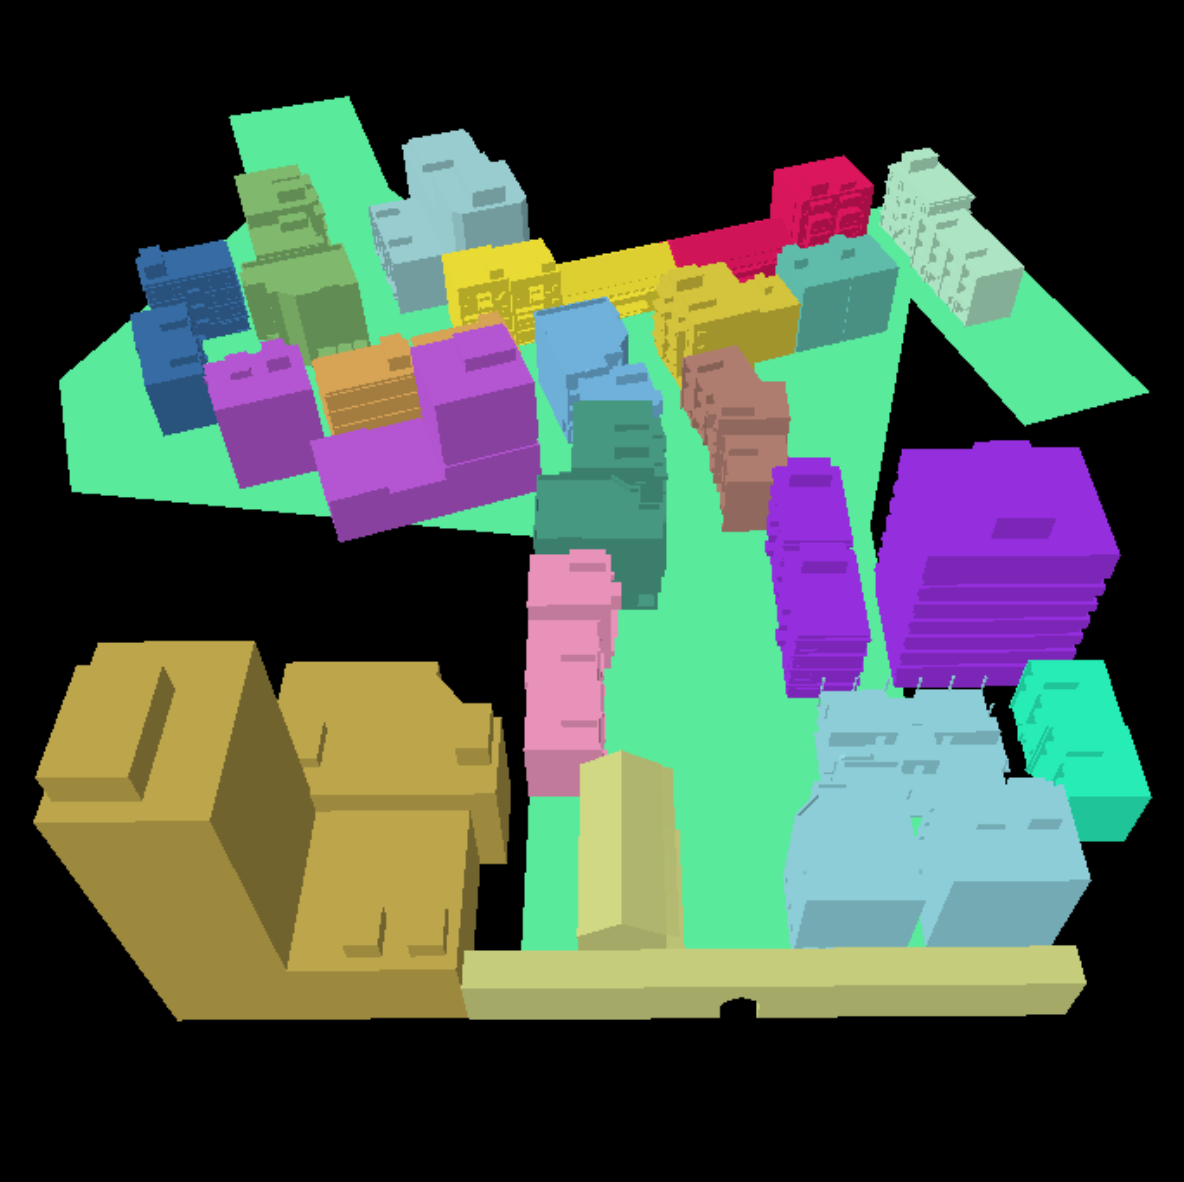
\includegraphics[width=1.\textwidth]{figures/r/path-30-1}
		\caption{系统}
	\end{subfigure}
	\begin{subfigure}[b]{0.285\textwidth}
		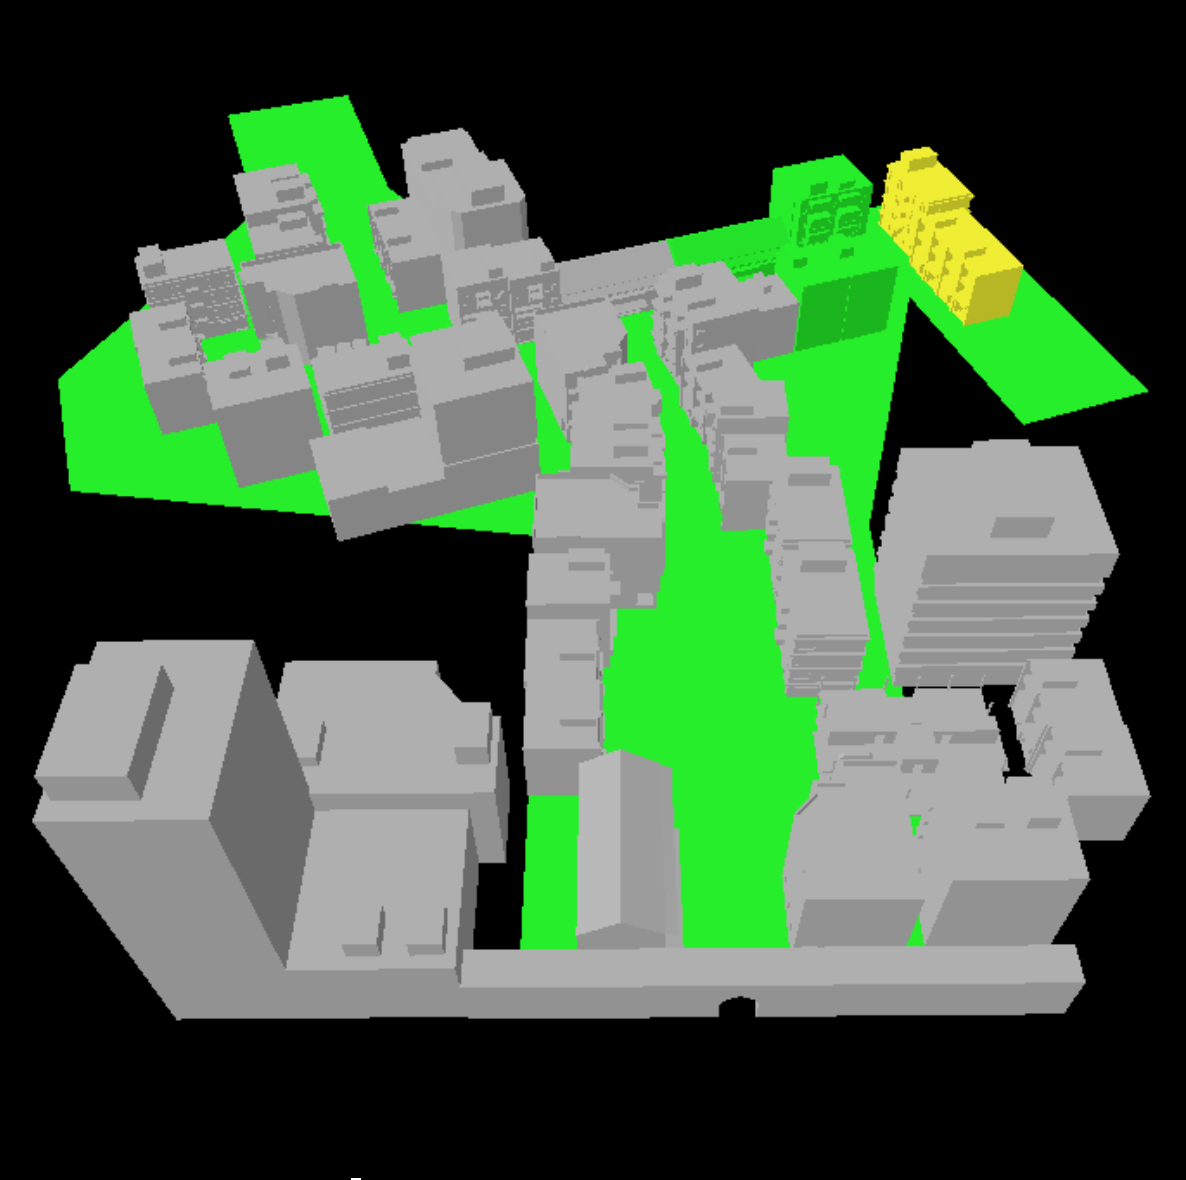
\includegraphics[width=1.\textwidth]{figures/r/path-30-2}
		\caption{系统依赖性}
	\end{subfigure}
	\begin{subfigure}[b]{0.42\textwidth}
		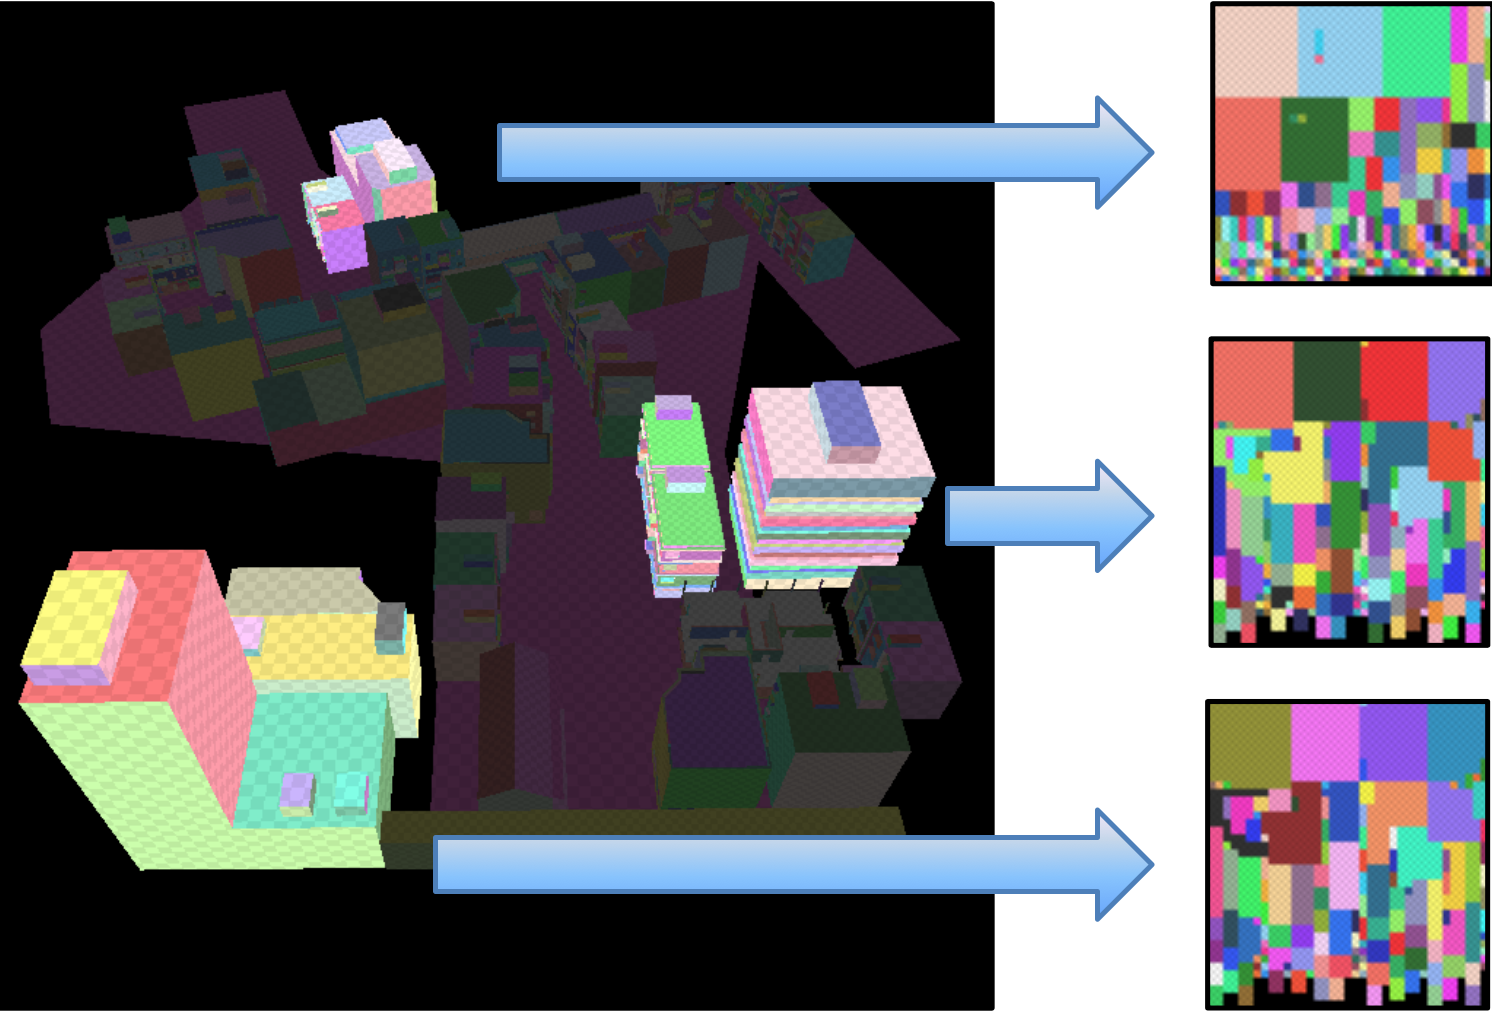
\includegraphics[width=1.\textwidth]{figures/r/path-30-3}
		\caption{光照贴图}
	\end{subfigure}
	\caption{辐射度系统划分(a),每个系统内的物体(或者说图表)共享一个光照贴图(c),系统之间存在着依赖关系(b),只有定义了相关性的系统之间才能够相互传输辐射度,每个系统内部的物体之间不存在辐射度光照的交互}
	\label{f:r-systems}
\end{figure}

系统的划分对计算效率起着关键作用。首先,各个系统之间可以相互独立地进行预处理,这提高了预处理和实时计算阶段多线程处理的效率;其次,系统之间存在相关性,例如在图\ref{f:r-scalings}(b)中,黄色系统内的物体的辐射度光照仅来自于绿色系统,其他所有系统(包含黄色系统自身)的遍历则可以被忽略;最后,系统的大小也被用于提高辐射度更新的性能,较大的系统拥有更多的像素,因此需要更长的处理时间,所以通过创建多个小的系统,辐射度光照更新可以被扩散到更多个时间帧中,可以提高游戏的实时性能。通过每个CPU每个时间帧处理一个系统。




\subsubsection{聚~~类}\label{sec:r-clustering}
聚类(clustering)\myindex{聚类}{clustering}阶段的主要内容是将几何场景细分成簇(cluster)\myindex{簇}{cluster},即辐射度方法中的细分曲面。

需要注意的是,簇和图表(光照贴图的UVs)以及光照贴图之间并无之间联系,它们之间仅仅只有一个相对关系,\textbf{Cluster Resolution}参数用于设置簇的尺寸相对光照贴图的分辨率,其默认值为0.5,这意味着一个簇的大小是光照贴图中一个像素的2倍大小。

Enlighten还使用了某种非连续网格化的方法对表面的可见性边界进行了区分。




\subsubsection{形状系数计算}
预处理的最后一个阶段用于计算簇之间的可见性信息,即形状系数。

Enlighten使用了局部线段的方法计算每个簇的形状系数,即从每个簇上向半空间发射光线,并统计落于其他簇上光线的数量来近似对应的形状系数。

为了使光线均匀分布于簇面上,Enlighten选择对光照贴图中每个像素所在的位置发射光线,其中参数\textbf{Irradiance Quality}控制着每个像素投射光线的数量,其默认值为8192,对该值的增加或减少只会影响形状系数的精度,并不会影响运行时的光照计算效率。

由此可知,光照贴图的分辨率影响着预处理的计算时间,更高的分辨率意味着更多的光线投射计算时间;另一方面,每个物体的光照贴图分辨率也影响其辐射度的精确度,例如低分辨率对应的像素数量更少,所以同样面积下投射的光线数量也更少,其辐射度精度也更低,因此低分辨率适合辐射度分布更平坦的区域,或者距离摄像机较远的区域,例如图\ref{f:r-chart-merging}(c)所示。

形状系数最终存储的精确度也受另一个参数的影响,即\textbf{Irradiance Budget},它表述每个簇存储的形状系数的数量,其默认值为128,Enlighten会尽可能多地合并一些簇之间的形状系数以满足这个预算要求,这有点类似小波辐射度方法中忽略掉一些高频的区域(例如那些距离较远的形状系数),而使用更平滑的结果来近似。由此表面Enlighten又某种类似阶层式辐射度方法的实现。




\subsection{实时计算阶段}
在实时计算阶段,Enlighten的主要任务是将一些输入数据转换为光照贴图,光照探针以及反射捕捉等数据供渲染引擎使用,如图\ref{f:r-enlighten-runtime}所示,其中光照贴图包含了间接漫反射信息,光照探针为动态或体积较小的物体提供了间接漫反射光照,而反射捕捉为光泽或镜面反射表面提供了间接漫反射环境。

 \begin{figure}
	\begin{center}
		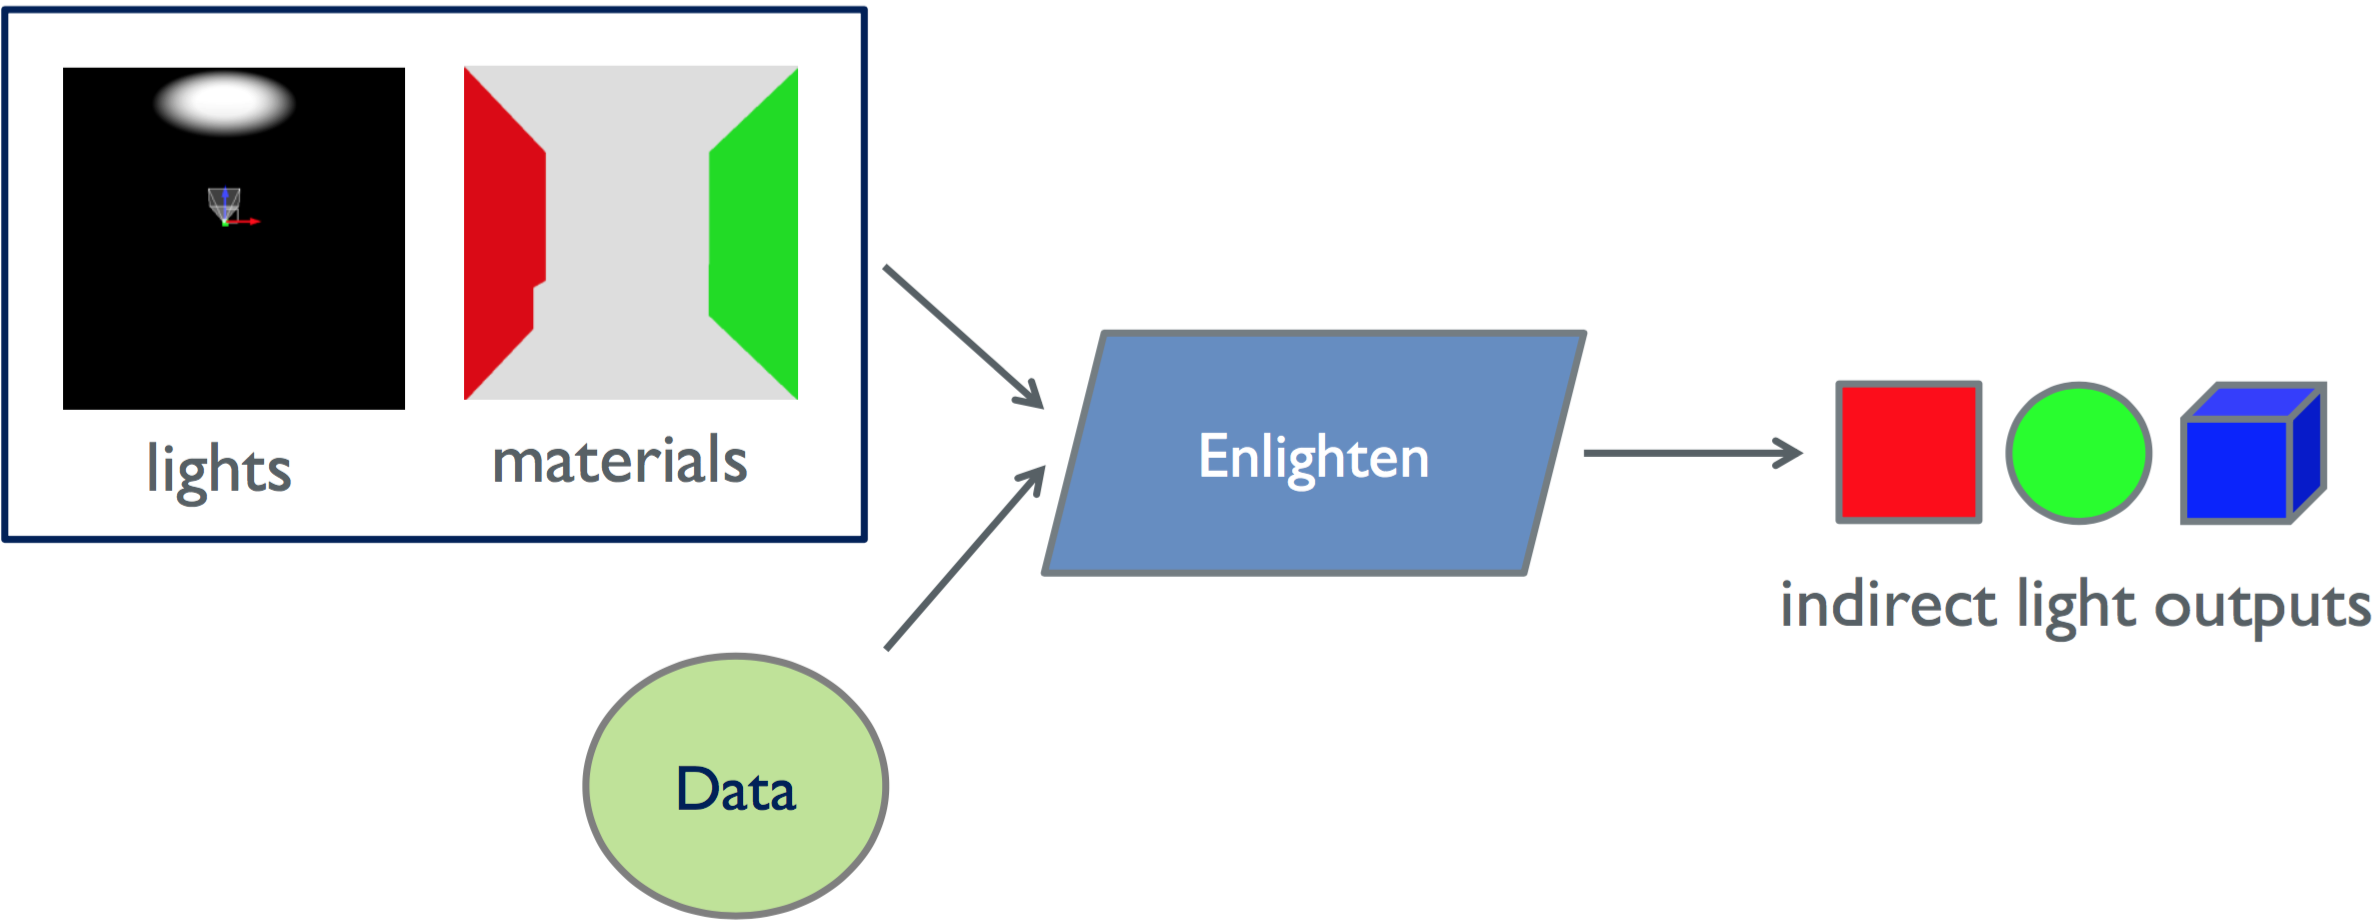
\includegraphics[width=0.9\textwidth]{figures/r/path-29-2}
	\end{center}
	\caption{Enlighten的运行时将动态的光照,材质等信息作为输入参数,结合预处理阶段存储的形状系数的信息,实时动态地计算场景的光照}
	\label{f:r-enlighten-runtime}
\end{figure}

由于Enlighten仅预处理与几何可见性相关的信息,所以(间接漫反射)光照计算中的任何其他参数均可以被动态修改,例如光源(包括环境光照)的光照密度,材质的漫反射系数,几何表面的自发光情况等,这给实时渲染带来了更多可能性。

在实时渲染中,直接光照通常能被图形处理器和渲染管线高效地处理,所以Enlighten运行时通常并不包含对直接光照的处理,因此Enlighten的输入不是直接对光源进行采样,而是对直接光照的“结果”进行采样,以保证仅处理二次以上的光线反弹。由于Enlighten只需要获得在细分曲面上的直接光照,所以它是对直接光照“结果”执行一个点采样(point sampling)来得到辐射度线性方程组的初始数据。由于光栅化得到的是一个2D的图像,而Enlighten的输入光照需要是物体表面的光照,其实是一张光照贴图,所以它应该是在这些点采样位置直接对光源采样以计算直接光照,此时仍然需要处理阴影遮挡的问题,由于曲面细分的分辨率要小得多,所以这个过程不会很耗时。也因此,仍以支持点采样的光源都可以被Enlighten使用,以及可以被动态修改。

Enlighten的实时光照计算是分多个迭代进行的,这得益于辐射度线性方程组的迭代式求解方式,这使得复杂的光照计算可以被分布到多个时间帧中,Enlighten每帧仅处理一个系统,从而不影响游戏其他渲染相关的工作。但是这种迭代的方式会使得起始阶段的品质较差,这也是Enlighten不能考虑直接光照的原因,但是随着时间的推进,Enlighten可以迭代处更好的品质。




\subsubsection{辐射度插值计算}
辐射度方法计算出的是一些离散的辐射度值,其中每个值表示曲面上一定面积内的平均辐射度值,我们需要得到曲面上连续平滑的辐射度分布,

假设曲面的辐射度度可以被线性近似,一个简单的方式是对曲面使用双线性插值(bilinear interpolation)\myindex{双线性插值}{bilinear interpolation},为了执行双线性插值,表示一个面积平均辐射度的辐射度值必须被转移到该曲面对应的顶点上去,例如图\ref{f:r-linear-extrapolation}所示。

\begin{figure}
\sidecaption
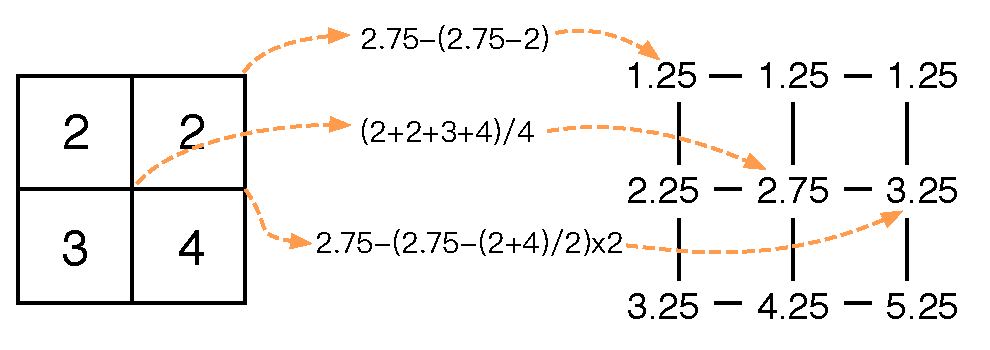
\includegraphics[width=0.65\textwidth]{figures/r/linear-extrapolation}
	\caption{辐射度方法计算的是一个曲面内的平均辐射度值,为了对曲面内其他顶点执行双线性插值,我们使用线性外推法推导出曲面顶点处的辐射度值}
	\label{f:r-linear-extrapolation}
\end{figure}

对于每一个几何曲面,其辐射度值表示的是该曲面内部区域内的平均辐射度值,我们可以使用一种称为线性外推(linear extrapolation)\myindex{线性外推}{linear extrapolation}的方法计算出每个顶点的辐射度值,线性外推与现场插值的过程相反,它们都保证数据成线性关系。例如每个顶点的辐射值可以为包含它的所有曲面的辐射度的平均值,如图\ref{f:r-linear-extrapolation}中间的顶点辐射度值为$2.75=(2+2+3+4)/2$,而其他边角位置顶点的值可以由其相邻顶点的值经过线性推导而出。线性外推具有以下定义:

\begin{equation}
	y=y_{k-1}+ \cfrac{x-x_{k-1}}{x_k-x_{k-1}}(y_k)-y_{k-1}
\end{equation}

\noindent 其中,$(y,x)$为未知量,它位于两个已知量$(x_{k-1},y_{k-1})$和$(x_k,y_k)$相连的线段上,上式可以求出给定任意位置$x$处的外推值$y$,并保证线性关系。






\section{实时动态辐射度方法}\label{sec:r-dynamic-radiosity}
虽然辐射度方法最初被设计为处理静态场景,但是相关领域也逐渐出现了一些衍变方法使其能够处理动态场景,其中\cite{a:Real-TimeDynamicRadiosityforHighQualityGlobalIllumination}更是几乎能够实时处理动态场景,本章最后一节来介绍一些实时动态辐射度方法相关的发展,思路以及方法。




\subsection{渐进式改进辐射度方法}\label{sec:r-progressive refinement-adiosity}
首先回顾一下传统的辐射度线性方程组:

\begin{equation}\label{e:r-gathering}
	B_i=B_{ei}+\rho_i \sum_j F_{ij} B_j
\end{equation}

\noindent 为了得到$B_i$的值,我们需要知道所有$B_j$的值,所以必须同时解决整个辐射度线性方程组,只有求解了整个线性方程组,才可以展示最终的渲染结果,这种方法很难满足交互操作的需求。

其中一个满足交互要求并保证图像质量的方法称为适应性改进(adaptive refinement)\myindex{适应性改进}{adaptive refinement}\cite{a:ImageRenderingbyAdaptiveRefinement},在该方法中,Bergman指出我们需要的是一个黄金线程(golden thread)\myindex{黄金线程}{golden thread},该线程是一个单一的操作,通过重复该操作,就能够持续地提升图像的质量,这种操作通过持续提升图像的质量而不是一次性地计算出最终结果,使图像能够被及时预览,因此能够满足交互操作。之后\cite{a:AProgressiveRefinementApproachtoFastRadiosityImageGeneration}对传统的辐射度算法进行修改,使其能够满足该黄金线程的要求。

\begin{figure}
\sidecaption
	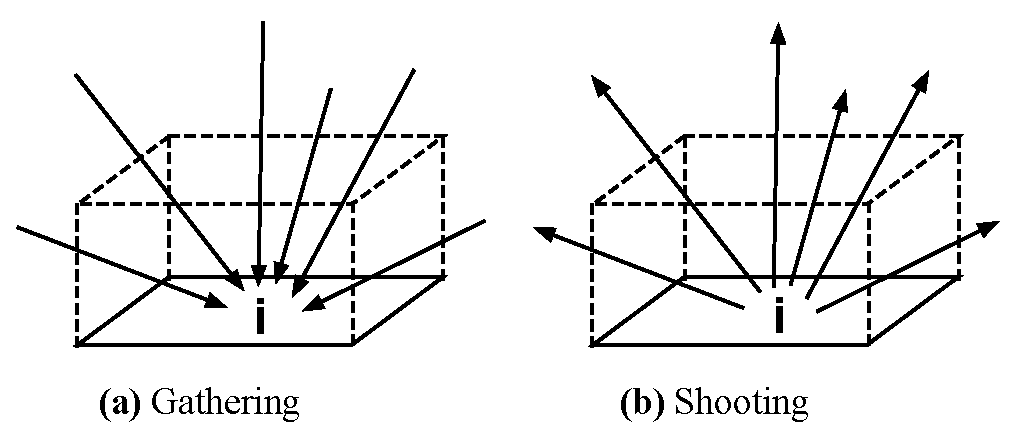
\includegraphics[width=.65\textwidth]{figures/r/shooting}
	\caption{曲面之间辐射度传输的两种方式,其中(a)收集来自其他曲面的光照,而(b)发射曲面的光照到所有其他曲面}	
	\label{f:r-gathering-and-shooting}
\end{figure}

在公式\ref{e:r-gathering}中,所有离开曲面$i$的光照来自于通过“收集”(gathering)\myindex{收集}{gathering}场景中其他曲面的光照,如图\ref{f:r-gathering-and-shooting}(a)所示。

式\ref{e:r-gathering}右边和式中的每一项表示曲面$i$的辐射度中来自曲面$j$的那一部分:

\begin{equation}
	B_i \text{ 来自于 }B_j=\rho_i B_j F_{ij}
\end{equation}

\noindent 我们可以将辐射度传输的过程反过来,即通过曲面$i$向所有其他曲面“发射”(shooting)\myindex{发射}{shooting}辐射度,如图\ref{f:r-gathering-and-shooting}(b)所示。形状系数的互反关系提供了这样的基础,曲面$j$的辐射度中来自于曲面$i$的部分可以表示为:

\begin{equation}\label{e:r-shooting}
	B_j\text{ 来自于 }B_i=\rho_j B_iF_{ij}A_i/A_j
\end{equation}

\noindent 上述的关系对所有曲面$j$都是成立的,即曲面$i$对整个场景的贡献可以表述为:

\begin{equation}\label{e:r-shooting}
	\text{对所有曲面$j$: } B_j\text{ 来自于 }B_i=\rho_j B_iF_{ij}A_i/A_j
\end{equation}

\noindent 对比式\ref{e:r-gathering}和式\ref{e:r-shooting}可以发现,前者需要存储所有的形状系数$F_{ij}$,而对于后者,虽然仍然需要计算每个$F_{ij}$,但是这些形状系数不需要被存储起来,因为在每一次迭代中,$F_{ij}$仅仅在计算曲面$i$向其他曲面$j$发射光照时使用,而每次迭代中曲面$i$仅被访问一次。所以,如果我们可以在每次遍历每个曲面的时候动态计算该曲面相关的形状系数,则内存中可以完全不需要存储任何形状系数。

此外,式\ref{e:r-shooting}还表明,对于每个曲面$i$,它能够同时计算该曲面对所有其他曲面的光照贡献,这意味每次处理完一个曲面我们就可以得到整个场景中每个曲面的辐射度值,因而得到一个图像结果,虽然该结果是不精确的,但是它提供了一种快速预览整个图像光照分布的能力,并且随着迭代的不断推进,整个图像的精确度不断提供并逐步收敛至较高的图像品质,这种渐进式的特征使辐射度方法具有了一定的交互性。

在整个迭代的过程中,每个曲面$i$都会被重复访问多次,每次迭代后由曲面$i$发射出的辐射度分布都会更加精确。但是,在前一次迭代中环境中已经包含了$B_i$的光照值,因此在下一次迭代中,只有两次迭代中曲面$i$的辐射度的差值$\triangle B_i$需要被考虑,$\triangle B_i$表述的是还未发射的辐射度,例如在曲面$i$上一次被访问之后由于其他曲面的访问向曲面$i$发射的光照。接受曲面$j$的由于曲面$i$的未发射增量可以表述为:

\begin{equation}\label{e:r-shooting}
	\text{来自曲面$i$的}\Delta B_j=\rho_j B^{u}_i F_{ij}A_i/A_j
\end{equation}

\noindent 其中,$B^{u}_i=\Delta B_i$,它表示曲面$i$全部未发射(unshot)的辐射度增量,当曲面$i$向所有其他曲面发射完毕之后该值被设为$B^{u}_i=\Delta B_i=0$。由此可以推断出,在迭代开始的时候$B_i=B^{u}_i=E_i$。

渐进式细分辐射度算法可由算法\ref{a:r-progressive-refinement}可见。

\begin{algorithm}
\begin{lstlisting}[language=C++, mathescape]
for each iteration, for each patch $i$ {
	//使用半立方体为曲面$i$计算所有形状系数
	$F_{ij}$ = CalculateFromHemiCubeAlgorithm();
	
	for each patch $j$ {
		//计算曲面$i$中未发射的辐射度对曲面$j$的贡献
		$\triangle Rad = p_j\triangle B_iF_{ij}A_i/A_j$;
		//曲面$j$中未发射的辐射度因为曲面$i$的贡献而被修改
		$\triangle B_j = \triangle B_j + \triangle Rad$; 
		//计算曲面$j$的所有辐射度,用于实时预览
		$B_i = B_j + \triangle Rad$; 
	}
	
	//曲面$i$的所有辐射度被发射之后将未发射辐射度设置为0
	$\triangle B_i = 0$; 
}
\end{lstlisting}
\caption{渐进式改进辐射度方法,每次迭代中形状系数被使用半立方体动态计算,辐射度被使用发射的方式每次由一个曲面发射向其他所有曲面,每次只发射自上次遍历之后发生改变的辐射度}
\label{a:r-progressive-refinement}
\end{algorithm}

上述的迭代过程不断进行,直到图像的品质收敛到一个满意的结果。每一次迭代都可以对所有曲面的辐射度同时进行更新,因此提供一些中间结果可以被显示预览,从而实现可交互。





\subsection{增量式辐射度方法}\label{sec:r-incremental-radiosity}
渐进式改进辐射度方法虽然到达了可交互的需求,但是同其他传统的辐射度方法一样,它要求被渲染的场景是静态的,如果场景的部分物体(的材质,位置,形状等)发生了改变,则整个迭代过程需要从头计算。渐进式改进辐射度方法并没有改善辐射度方法的计算内容,或者我们可以认为它仅是换一种角度看待同一计算过程。

然而,渐进式改进辐射度方法提出了一种非常适合动态场景的辐射度传输方式,由于在每次迭代中,曲面的辐射度可以分为已发射和未发射辐射度的和,因此对于动态场景,如果我们能够把由于场景的动态修改操作导致辐射度的修改转换为曲面的未发射辐射度,则我们就可以在不需要重启整个迭代过程的情况下适应场景的动态调整。

基于此,\cite{a:IncrementalRadiosity:AnExtensionofProgressiveRadiositytoanInteractiveImageSynthesisSystem}提出了一个渐进式改进辐射度方法的扩展方法,称为增量式辐射度方法(incremental radiosity)\myindex{增量式辐射度方法}{incremental radiosity},该方法能够基于场景或材质属性的改变增量式的(而不是从头开始)渲染场景。这个方法大大减少了一些不必要的计算时间,换句话说,增量式辐射度方法考虑的是:对于开关光源,修改表面漫反射颜色,添加或移除物体这样对场景的修改操作,响应这些修改需要的最小计算量是什么?

增量式辐射度算法和传统的渐进式改进辐射度算法的结构类似,但是在每个迭代开始的时候,它会检测每个对场景的修改操作,如果一个修改操作被请求,则迭代过程会被暂停,以处理这些修改操作,并在处理完毕之后恢复迭代过程。这些被允许的修改操作包括物体表面的材质属性,自发光情况,以及对几何物体的修改,以下分别讨论。




\subsubsection{表面材质属性的修改}
当物体的表面属性(例如自发光情况或漫反射系数)发生修改时,我们只需要求出这些修改操作导致该表面的辐射度增量即可,这个增量会在后续的迭代过程中被传播出去。

表面属性的修改导致的辐射度增量可以分为自发光属性和漫反射系数的修改两类情况,设$B^{'}_{ei}$和$\rho^{'}_i$为修改后的自发光辐射度和漫反射系数,则曲面$i$因为表面属性修改的辐射度增量为:

\begin{equation}
	\triangle B_i=B^{'}_{ei}-B_{ei}+ \cfrac{(\rho^{'}_i-\rho_i)(B_i-B_{ei})}{\rho_i}
\end{equation}

\noindent 上式的推导可参见\cite{a:IncrementalRadiosity:AnExtensionofProgressiveRadiositytoanInteractiveImageSynthesisSystem,a:ImprovingInteractionWithRadiositybasedLightingSimulationPrograms}。该式其实非常好理解,第一项$B^{'}_{ei}-B_{ei}$表示的是自发光属性修改导致的辐射度增量,对于第二项,由于曲面$B_i$表示从迭代开始后到目前为止它总共的辐射度,其中$B_i-B_{ei})$表示的是来自其他曲面的辐射度,并且这部分辐射度是以$\rho_i$为反射系数计算的,所以上式第二项的意义就是将这部分辐射度改为以$\rho^{'}_i$为反射系数计算的辐射度增量。




\subsubsection{几何属性修改}
与表面属性的修改不同,几何属性的修改往往会涉及形状系数的修改,尽管增量式辐射度方法仍然提出了增量式形状系数(incremental form factor)\myindex{增量式形状系数}{incremental form factor}的概念以计算几何修改导致的辐射度增量,但是其计算相对复杂,下一节介绍的重分配辐射度方法从数学公式上更好地解释了这种几何属性修改导致的辐射度增量,因此我们仅在下一节讨论后者。





\subsection{辐射度重分配}\label{sec:r-radiosity-redistribution}
对于几何属性的修改,\cite{a:RadiosityRedistributionforDynamicEnvironments}提出了一个更好的数学描述,称为辐射度重分配(radiosity redistribution)\myindex{辐射度重分配}{radiosity redistribution},在辐射度重分配方法中,一个称为重分配(redistribution)\myindex{重分配}{redistribution}的操作被用于计算由于几何属性修改对曲面出射辐射度能量的修正。场景中物体的添加,移除,移动以及修改等操作都会导致辐射度能量被重分配。

辐射度重分配的数学公式可由经典辐射度公式推导而来。在辐射度方程中,对于物体几何属性的修改,我们可以设置一个时间相关的变量作为变量上标,时间$t-1$表示原始(修改前的)辐射度方程,而修改后新的辐射度方程的时间值为$t$,所以上标$\Delta t$表示时间$t-1$到$t$之间的与时间相关变量的增量。

基于以上的概念,我们可以重写(修改前后的)一般的辐射度方程为:

\begin{equation}
	\begin{aligned}
		&B^{t-1}_i=E_i+\rho_i \sum^{n}_{j=1}F^{t-1}_{ij}B^{t-1}_j\\
		&B^{t}_i=E_i+\rho_i \sum^{n}_{j=1}F^{t}_{ij}B^{t}_j
	\end{aligned}
\end{equation}

\noindent 利用关系$B^{t}_i=B^{t-1}_i+B^{\triangle t}_i$以及$F^{t}_{ij}=F^{t-1}_{ij}+F^{\triangle t}_{ij}$可以得到:

\begin{equation}\label{e:r-difference-of-radiosity}
	B^{\triangle t}_i=\rho_i\sum^{n}_{j=1}F^{\triangle t}_{ij}B^{t-1}_i+\rho_i\sum^{n}_{j=1}F^{t}_{ij}B^{\triangle t}_i
\end{equation}

\noindent 我们定义右式中第一项为一个重分配项(redistribution term)\myindex{重分配项}{redistribution term},记为$R_i$,则有:

\begin{equation}\label{e:r-redistribution-term}
	R_i=\rho_i\sum^{n}_{j=1}F^{\triangle t}_{ij}B^{t-1}_i
\end{equation}

\noindent 将上式代入式\ref{e:r-difference-of-radiosity}则得到辐射度重分配方程:

\begin{equation}\label{e:r-redistribution-equation}
	B^{\triangle t}_i=R_i+\rho_i\sum^{n}_{j=1}F^{t}_{ij}B^{\triangle t}_i
\end{equation}

\noindent 如果场景不发生任何修改,则上式只剩下右边的项,如果场景发射修改,则其形状系数会发生变化,只要我们计算出修改之后的形状系数$F^{t}_{ij}$,则它可以和正常的辐射度方法一样被计算。我们需要关注的是重分配项。

所谓重(英语前缀re-)的概念,是指对已经做过的事情或执行过的动作重做一次,重做的方法可能不一样以产生不同的结果,但是这件事情需要再执行一次。尽管我们将辐射度传播的过程转换为多个迭代的过程,但其实辐射度的传输是瞬时的,例如打开灯的开关就会瞬间照亮房间,我们对场景的修改时刻不可能处于辐射度的传播过程当中,这意味着假设我们在某次迭代中接收到修改请求,实际上我们应该返回到开头以新的几何条件重新执行辐射度的传输迭代过程。

如果我们将曲面$i$直接回滚到迭代初始,则整个场景的光照分布都会受到影响,因而全部曲面的光照传输都需要从新开始。然而有了增量式辐射度的概念,我们便可以只需要将曲面$i$由于几何属性修改导致的辐射度增量求出来即可,这即是重分配项,其中$B^{t-1}_i$累积了曲面$i$在该次迭代之前收到的所有辐射度,将这部分辐射度乘以形状系数增量$F^{\Delta t}_{ij}$即得到了由于几何属性修改导致的辐射度增量。

有了式\ref{e:r-redistribution-equation}的表述,剩下最重要的任务就是计算场景中所有由于几何属性修改导致的重分配项。虽然\cite{a:RadiosityRedistributionforDynamicEnvironments}包含重分配项的计算,但是其计算复杂度比较高,其原因会在下节分析,这里我们直接介绍计算效率更高的交叉重分配方法。




\subsection{交叉重分配辐射度方法}\label{sec:r-cross-edistribution-adiosity}
基于上述的动态辐射度技术,\cite{a:Real-TimeDynamicRadiosityforHighQualityGlobalIllumination}提出了交叉重分配辐射度方法(cross redistribution radiosity)\myindex{交叉重分配辐射度方法}{cross redistribution radiosity},以下我们首先对重分配辐射度方法的理论基础做一些分析,然后结合增量式辐射度方法的一些观察推导出本节要介绍的交叉重分配辐射度方法。



\subsubsection{Requirements for Adaptivity}
当一个几何属性修改之后,所有涉及改变的曲面之间的辐射度传输都需要被修正,即上节介绍的重分配,为此我们定义一个重分配函数(redistribution function)\myindex{重分配函数}{redistribution function} $\mathbf{R}(X,Y)$ 以兼顾所有的几何属性修改。这里$X$表示所有发射辐射度的曲面,$Y$表示所有接受辐射度的曲面,注意每个曲面都可能既是发射曲面,又是接受曲面。

式\ref{e:r-basic-redistribution}是重分配函数$\mathbf{R}_g(X,Y)$的一个基本实现,其矢量标记用于包括所有曲面$Y$,该式的值是一个表示辐射度差异值(增量)的矢量,用于定义所有曲面$Y$的重分配辐射度:

\begin{equation}\label{e:r-basic-redistribution}
	\mathbf{R}_g(X,Y)=\Biggr\{ \rho_i\sum_{j\in X}B^{s}_j \bigtriangleup F_{ij} \Biggr\}_{i\in Y}
\end{equation}

\noindent 上式中小标$g$表示传统的使用收集的辐射度方法,$B^{s}_j$表示已发射辐射度。直观上理解,该式对使用旧(修改之前)的形状系数进行传输的辐射度进行修改,使其结果就像是被使用新(修改之后)的形状系数进行传输的。

我们定义包含所有曲面的集合为$P$,并将所有这些曲面分为两类曲面的集合,即未发生修改的静态曲面集合$C$,以及发生修改的动态曲面集合$M$,显然这里满足$P=C\cup M$。

根据上述的曲面分类,我们可以将重分配函数分解为四个部分,即$\mathbf{R}(C,M)$, $\mathbf{R}(M, C)$, $\mathbf{R}(M, M)$和$\mathbf{R}(C, C)$,因此总的重分配函数可修改为:

\begin{equation}
	\mathbf{R}(P, P)=\bigg( \mathbf{R}(C,M)+\mathbf{R}(M,M)+\mathbf{R}(M,C)+\mathbf{R}(C,C) \bigg)
\end{equation}

\noindent 这样分类的四个重分配函数都有其独特的属性:

\begin{itemize}
	\item $\mathbf{R}(C,M)$:由于$M$的位置和方向等几何属性发生变化,所有由曲面$C$向曲面$M$传输辐射度的形状系数都发生了变化。
	\item $\mathbf{R}(M,C)$:跟$\mathbf{R}(C,M)$类似,所有由曲面$M$向曲面$C$传输辐射度的形状系数都会发生变化。 
	\item $\mathbf{R}(M,M)$:大多数情况下$M$与$M$之间的形状系数都会发生变化,但是有一种特例,如果$M$和$M$均以相同的刚体变换,此时两者之间的形状系数保持不变,除非两者之间的可见性由于其他不相关曲面发生了变化。
	\item $\mathbf{R}(C,C)$:只有两者之间的可见性发生变化时,才会导致两者之间的形状系数发生变化,此时引入可见性变化的不相关曲面一定位于$M$中。
\end{itemize}

需要注意的是,对于连续多个几何属性的修改,需要确保这些修改导致的重分配操作被按修改事件发生的时间顺序执行,因为每个重分配操作是一个不可分割的整体,否则将导致辐射度不能被正确重分配。

另一点需要注意的是,由于整个算法是增量式的,即在当前结果上进行增量修改,而不是重新计算整个辐射度传输过程。所以,如果辐射度重分配过程中使用了某些近似方法,则一些小小的近似误差可能在后续许多重分配迭代过程中被放大,所以需要较高精度的重分配算法以避免这种累积放大的误差。




\subsubsection{增量式辐射度方法分析}
式\ref{e:r-progressive-redistribution}定义了一个渐进式版本的重分配函数$\mathbf{R}_p(X,Y)$,即:

\begin{equation}\label{e:r-progressive-redistribution}
	\mathbf{R}_p(X,Y)=\sum_{j\in X}\Biggr(\Biggr\{ \rho_i B^{s}_j \bigtriangleup F_{ji} \cfrac{A_j}{Ai} \Biggr\}_{i\in Y}\Biggr)
\end{equation}

\noindent 这里小标$p$表示渐进式的(progressive),直观上理解,上式从曲面$j$向所有其他接收曲面$i$发射重分配辐射度,并对所所有发射曲面重复此操作形成一个矢量值结果。

在前面介绍的增量式辐射度方法中,为了发射辐射度到其他所有接收曲面,一个半立方体在发射曲面上被建立以计算所有形状系数,如图\ref{f:r-gathering-and-shooting}(b)所示。为了计算增量式形状系数$\Delta F_{ji}$,这里需要使用两个半立方体,其中一个用于计算修改前的形状系数,而另一个用于计算修改后的形状系数。更确切地说,$2\cdot|M|$个半立方体被完全渲染,而$2\cdot |C|$个半立方体被部分渲染(为修改的静态物体仅与少数动态物体之间的形状系数发生修改,半立方体的很多像素值保持不变),总的计算复杂度为$O(2|M|+2|C|)$。而根据本书前面硬件相关的内容可知,部分渲染的半立方体在图像硬件上的执行效率非常低。

在下一节中,我们将介绍一种交叉重分配辐射度方法,该算法可以达到一半立方体计算$O(4|M|)$的计算复杂度,在一般的场景中通常中满足$|M|\ll|C|$,所以这可以大大提升重分配的计算效率。




\subsubsection{交叉重分配辐射度方法}
交叉重分配方法并不会为每个静态曲面$C$渲染一个半立方体,而是仅针对每个动态曲面$M$渲染一个半立方体。为了达到这样的要求,重分配方法必须被执行一定的重构。

在渐进式重分配函数中,$\mathbf{R}_p(M,C)$和$\mathbf{R}_p(M,M)$本身是仅针对所有动态曲面$M$渲染半立方体的;对于$\mathbf{R}(C,M)$,我们可以使用基于收集的重分配函数$\mathbf{R}_g(C,M)$,因为该函数对所有接受面$M$渲染一个半立方体。

重分配函数$\mathbf{R}(C,C)$是最具挑战的,不管基于收集的重分配函数方法还是渐进式重分配函数均需要针对所有静态曲面$C$渲染一个半立方体,而新的交叉重分配函数$\mathbf{R}_x(C,C)$就是要在计算所有静态曲面$C$之间的重分配辐射度传输的同时,仅仅对所有动态曲面$M$渲染一个半立方体。

\begin{figure}
	\sidecaption
		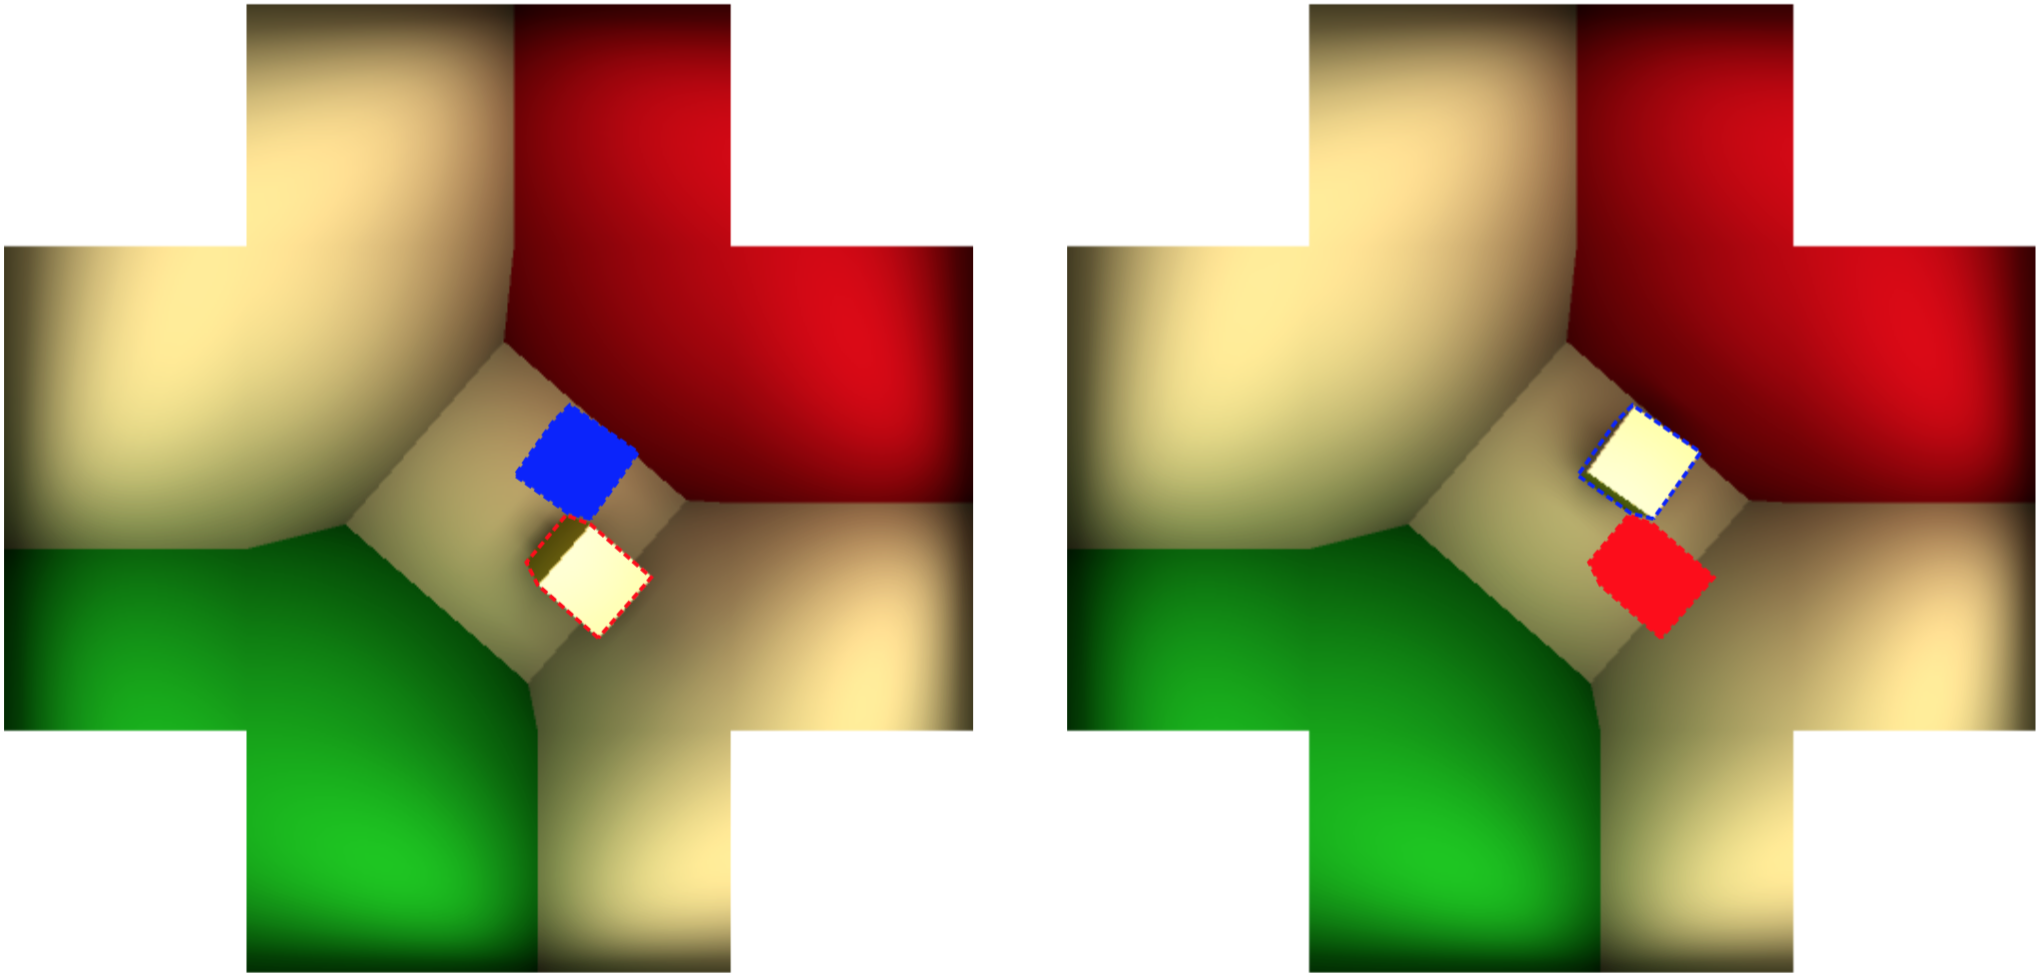
\includegraphics[width=0.65\textwidth]{figures/r/path-38}
	\caption{场景被修改前(左)和后(右),其透明区域(蓝色和红色区域)分别为位于$\mathbf{R}_p(C,C)$中的一个发射曲面渲染一个半立方体,其中红色区域表示未被遮挡,而蓝色被遮挡了(图片来自\cite{a:Real-TimeDynamicRadiosityforHighQualityGlobalIllumination})}
	\label{f:r-two-hemicubes}
\end{figure}

一个重要的观察是所有的重分配辐射度都要经过被修改曲面$M$的旧(修改前)或者新(修改后的)位置,因为其他静态曲面$C$之间的形状系数保持不变(因此不存在重分配辐射度项),这是交叉式重分配辐射度方法的重要基础。对于静态曲面$i$(位于$C$中),其辐射度的重分配可以通过所有$i$可见的动态曲面$j$(位于$M$中)来实现,例如图\ref{f:r-two-hemicubes}中的透明(蓝色和红色)区域。

当从动态曲面$M$观察式,其重分配辐射度穿过其中形成一个交叉的形状\footnote{为了便于理解,这里“交叉”是指这些静态的曲面(如$r,g,b$)通过动态曲面($j$)然后交叉于另一个静态曲面$i$。},因此被称为交叉投影,注意交叉投影重分配函数仅被运用于$\mathbf{R}(C,C)$类型的重分配。

\begin{figure}
\sidecaption
	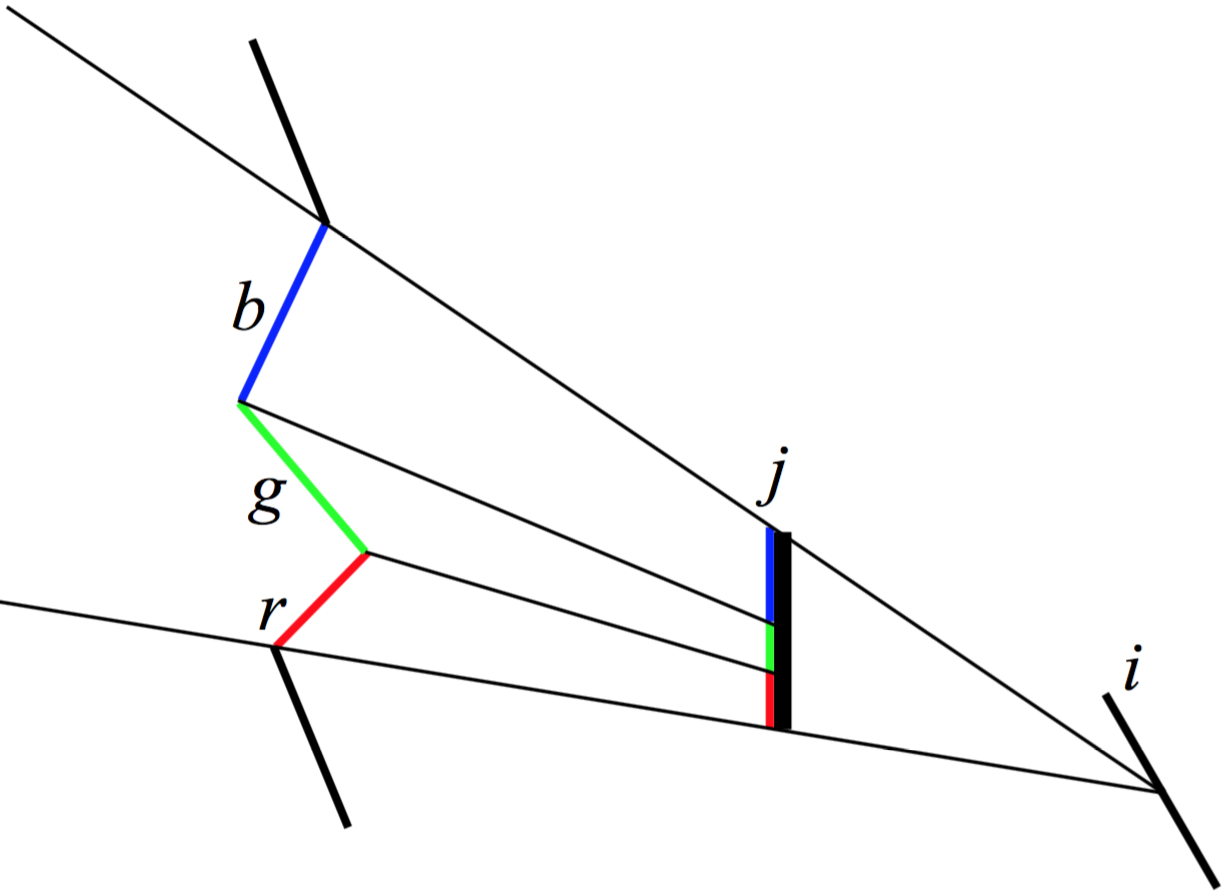
\includegraphics[width=.5\textwidth]{figures/r/path-39}
	\caption{交叉投影重分配的示例,其展示了中间投影的概念,这里$M = \{j\}$,$C = \{r,g,b,i,...\}$}
	\label{f:r-c-c}
\end{figure}

图\ref{f:r-c-c}描述了一部分静态曲面($r,g,b\in C$)到另一个通过动态曲面$j\in M$可见的静态曲面$i\in C$的重分配函数$\mathbf{R}_x(C,C)$, 为了计算它们之间的重分配辐射度,一个中间过程被引入,其中$r,g,b$部分的辐射度被使用一个以$i$为原点的透视投影投射到曲面$j$上,然后曲面$j$上的辐射度被传输到曲面$i$上。

对于具有相同原点的半立方体,由于多个具有相同投影面积的曲面拥有相同的形状系数,所以很容易从图\ref{f:r-c-c}看出以下的组合形状系数关系$F_{ij}=F_{ir}+F_{ig}+F_{ib}$,换句话说,曲面$r,g,b$传输到曲面$j$然后再传输到曲面$i$的辐射度,等于由曲面$r,g,b$直接传输到曲面$i$的辐射度。

最终由曲面$j$传输到曲面$i$的重分配辐射度等于$\mathbf{R}(M,C)$,该项值可以通过渐进式重分配函数$\mathbf{R}_p(M, C)$计算。

式\ref{e:r-cross-redistribution-radiosity}给出了交叉重分配辐射度函数的公式,该公式与渐进式重分配函数$\mathbf{R}_p(M,C)$(式\ref{e:r-progressive-redistribution})是相似的,只不过这里已发射辐射度$B_j^{s}$被一个投影辐射度函数$P(C,j,i)$取代。

\begin{equation}\label{e:r-cross-redistribution-radiosity}
	\mathbf{R}_x(C,C)=\sum_{j\in M}\bigg(\bigg\{\rho_i \cfrac{A_j}{A_i}(-F^{'}_{ji}P(C,j^{'},i)+F_{ji}P(C,j,i))\bigg\}_{i\in C}\bigg)	
\end{equation}
